% Document class, language and encoding setup
\documentclass[a4paper,12pt,danish]{report}

\usepackage[danish]{babel}
\usepackage[utf8]{inputenc}
\usepackage[T1]{fontenc}
% Fixing the font issue
\usepackage{ae,aecompl}

% Color package
\PassOptionsToPackage{dvipsnames}{xcolor}
	\RequirePackage{xcolor} % [dvipsnames] 
	
% Allows page-links in pdf file
\usepackage[colorlinks=true]{hyperref}

\usepackage{pdfpages}
% Todo notes package and commands
\usepackage{todonotes}
% Allows commands to emit a space "at the end"
\usepackage{xspace}

% Listings setup
\usepackage{listings}

% Graphics setup
\usepackage{graphicx}
\graphicspath{{./graphics/}{./graphics/sensor/}}

\usepackage{tikz}
\usepackage{3dplot}

\usetikzlibrary{calc}
\usepackage{amsmath}
\usepackage{amssymb}

% Advanced tables
\usepackage{tabularx}
\usepackage{multirow}

% Clever references
\usepackage{cleveref}

% Bibliography
\usepackage[square,numbers]{natbib}
\bibliographystyle{plainnat}

% Force position [H]
\usepackage{float}

% For figures with sub-figures
\usepackage{subcaption}

% Tikz
\usepackage{tikz}
\usetikzlibrary{arrows,backgrounds,snakes}
 
% Additional commands
\newcommand{\namedtodo}[5]
{
  \ifthenelse{\equal{#1}{}}
  {
    \todo[color=#4,caption=
    {\textbf{#3: } #2}
    ,inline]
    {\color{#5}\textbf{#3: }#2}
  }
  {
    \todo[color=#4,caption=
    {\textbf{#3: } #1}
    ,inline]
    {\color{#5}\textbf{#3: }#2}
  }
}
\newcommand{\mikkel}[2][]{\namedtodo{#1}{#2}{Mikkel}{blue!80}{white}}
\newcommand{\stefan}[2][]{\namedtodo{#1}{#2}{Stefan M}{orange}{black}}
\newcommand{\anders}[2][]{\namedtodo{#1}{#2}{Anders}{orange}{black}}
\newcommand{\thilemann}[2][]{\namedtodo{#1}{#2}{Stefan T}{NavyBlue!35}{NavyBlue}}
\newcommand{\mikael}[2][]{\namedtodo{#1}{#2}{Mikael}{green}{black}}
\newcommand{\bruno}[2][]{\namedtodo{#1}{#2}{Bruno}{black!10!red!90}{white}}
% Her er en liste over navnene p� de forskellige styles
% C#: csharp
% F#: fsharp

% 
% Listings kan refereres vha. \cref{}
\crefname{listing}{kode eksempel}{kode eksempler}
\Crefname{listing}{Kode eksempel}{kode eksempler}
% 

\lstdefinestyle{standard}
{
	frame=shadowbox,
	framesep=5pt,
	rulecolor=\color{blue!40!black},
	rulesepcolor=\color{white!93!black},
	basicstyle=\ttfamily\normalsize,
	numbers=left,
	numberstyle=\tiny,
	numberfirstline=true,
	%numberblanklines=false,
	stepnumber=1,
	numbersep=9pt,	
	captionpos=b,
	escapeinside={(*}{*)}
}

\lstdefinestyle{c}
{
	style=standard
}

\lstdefinestyle{csharp}
{
	style=standard,
	language=[Sharp]C
}
\lstdefinestyle{csharpsmall}
{
	style=csharp,
	basicstyle=\ttfamily\footnotesize
}
\lstdefinestyle{fsharp}
{
	language=[Sharp]F,
	frame=lr,
	rulecolor=\color{blue!80!black}
}
\lstdefinestyle{fsharpsmall}
{
	style=fsharp,
	basicstyle=\ttfamily\footnotesize
}
%Definitions
\newcommand{\mindsqualls}{MindSqualls\xspace}
\newcommand{\csharp}{\textsc{C\#}\xspace}
\newcommand{\fsharp}{\textsc{F\#}\xspace}
\newcommand{\legoms}{\textsc{LEGO\textregistered{} MINDSTORMS\textregistered{}}\xspace}
\newcommand{\lego}{\textsc{LEGO$^{\textrm{\scriptsize\textregistered}}$}\xspace}
\newcommand{\legos}{\textsc{LEGO$^{\textrm{\scriptsize\textregistered}}$s}\xspace}
\newcommand{\kinect}{\textsc{Kinect\texttrademark{}\xspace}}

%Superscript and subscript
\newcommand{\superscript}[1]{\ensuremath{^{\textrm{#1}}}}
\newcommand{\subscript}[1]{\ensuremath{_{\textrm{#1}}}}

% Degrees
\newcommand{\degree}{\ensuremath{^\circ}}
\newcommand{\dg}{\degree}

%Blank page
\newcommand{\blankpage}{\newpage\mbox{}\newpage}

\begin{document}
\listoftodos[Todo liste]
%Front page
\begin{titlepage}
\newcommand{\HRule}{\rule{\linewidth}{0.5mm}}

\begin{center}

\HRule \\[0.5cm]
\textsc{ \Huge Mapping med LEGO-robot}\\

\HRule \\[1cm]

\textsc{\Large SW505E13} \\[2cm]

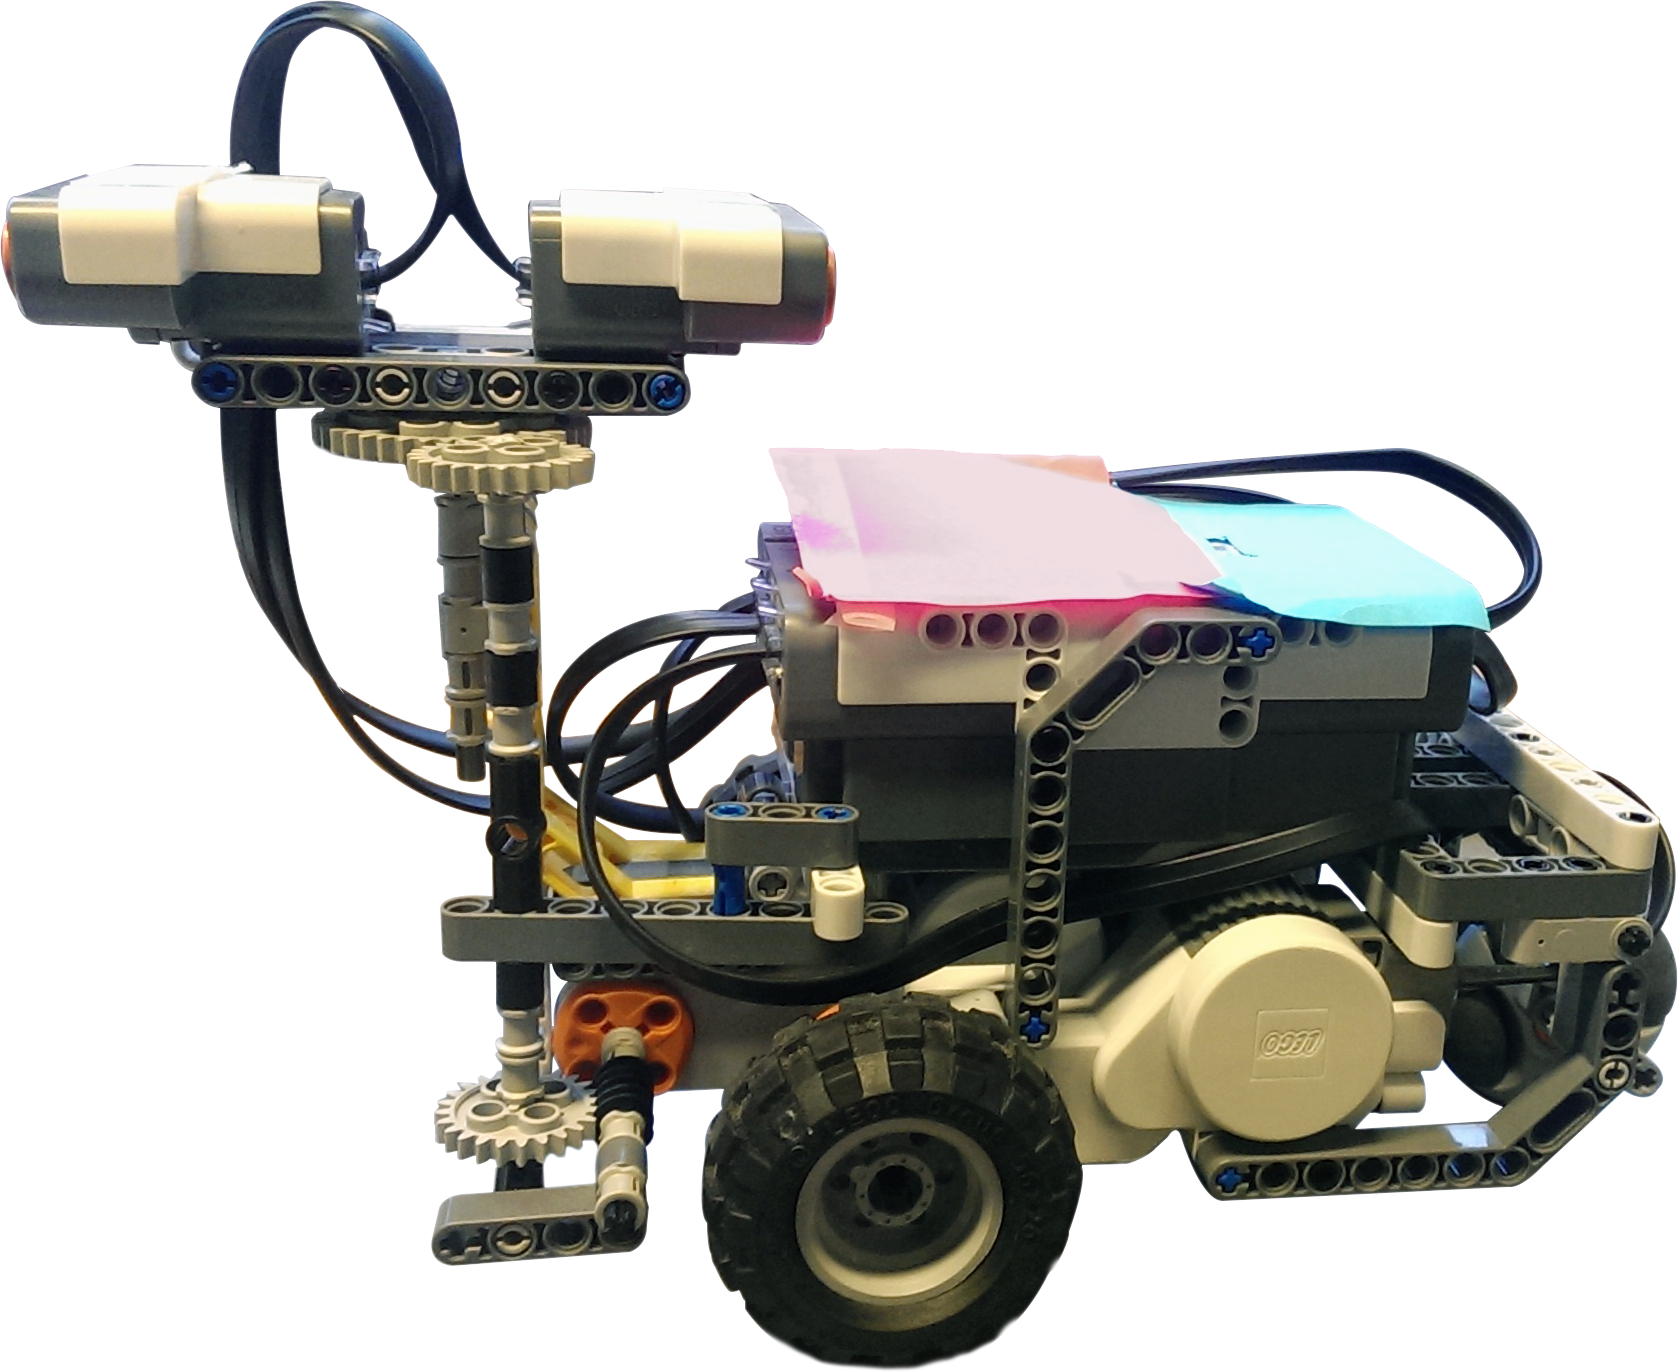
\includegraphics[width=.8\textwidth]{whalle}

\vfill
{\Large Indlejrede systemer}
\\ ~\\
{\large Efterårssemesteret 2013}

\end{center}
\end{titlepage}

\pagenumbering{Roman}

\clearpage

\thispagestyle{empty}
\begin{titlepage}
\setlength{\textwidth}{15cm}
	\noindent
\begin{nopagebreak}
{\samepage 
\begin{tabular}{r}
	\parbox{15cm}{\raisebox{11mm}{
\includegraphics[height=1.2cm]{./graphics/aauLogoDa.jpg}}
	\hfill \parbox{7cm}{\begin{tabular}{l}
		{\small \textbf{Institut for Datalogi}}\\
		{\small Selma Lagerløfs Vej 300} \\
		{\small 9220 Aalborg Ø} \\
		{\small Phone (+45) 9940 9940} \\
		{\small Fax (+45) 9940 9798} \\
		{\small http://cs.aau.dk}
	\end{tabular}}
.	}
\end{tabular}

\begin{tabular}{cc}
	\parbox{8cm}{
	\begin{description}
		\item { \textbf{Titel:}}\\ 
			Mapping
    		\item { \textbf{Tema:}}\\ 
			\raggedright Indlejrede systemer
	\end{description}
	
	\parbox{8cm}{
	\begin{description}
		\item { \textbf{Projektperiode:}}\\
			01-09-2013 -\\
			20-12-2013
 		\hspace{4cm}
		\item { \textbf{Projektgruppe:}}\\
  			sw505f13
 		\hspace{4cm}
		\item {\textbf{Deltagere:}}\\
			Anders R. Nielsen\\
			Bruno Thalmann\\
			Mikael E. Christensen\\
			Mikkel S. Larsen\\
			Stefan M. G. Micheelsen\\
			Stefan M. Thilemann\\
		\hspace{2cm}
		\item { \textbf{Vejleder:}}\\
 			Nicolaj Søndberg-Jeppesen\\
  	\end{description}
	}
	\begin{description}
		\item { \textbf{Printings:} 2}
		\item { \textbf{Pages:} \pageref{LastPageBody} } 
		\item { \textbf{Appendices:} 40}
		\item { \textbf{Total pages:} \pageref{LastPage} }
		\item { \textbf{Source code:} See CD-ROM}
		\bruno{husk at opdatere dette.}
	\end{description}
	\vfill } &
	\parbox{6.5cm}{
 	 \vspace{.15cm}
  	\hfill 
  	\begin{tabular}{l}
  		{Abstract:}\bigskip \\
  		\fbox{
  		\parbox{6cm}{\bigskip
     		{\vfill{\small \paragraph{Purpose:}The purpose of this project was to map an unknown area, using a robot (mapping) which knows it's location.

\paragraph{Method:}To accomplish this, a robot was built using \legoms, consisting of a rotating ultra-sonic-sensor-construction built on top of a tripod.
The purpose of the robot was to navigate and collect sensor measurements and provide these to a PC, which would construct a map based on the supplied data.
This would result in a continuously updated occupancy grid, using a sensor model (both simple and Gaussian variants).
Additionally, as a simplification of the problem, the PC would supply the robot with its location and orientation (pose), based on color-tracking a live stream from a Kinect, whenever needed.

\paragraph{Results and conclusion:}
\mikael{Noget test-resultat og konklusion}
     		\bigskip}}
     	}}
   	\end{tabular}}
\end{tabular}
\noindent{\footnotesize{\textit{Rapportens indhold er frit tilgængeligt, men offentliggørelse (med kildeangivelse) må kun ske efter aftale med forfatterne.}}}
}%samepage end
\end{nopagebreak}
\end{titlepage}
\clearpage

\setcounter{page}{4}
\setcounter{secnumdepth}{3}

\newcommand{\prefaceHeaderName}{Forord}
\section*{\prefaceHeaderName}
Denne rapport er udarbejdet af Software-Ingeniør studerende på 5. semester, på Aalborg Universitet, efterårssemesteret 2013.
Det forventes at læseren har en baggrund indenfor IT/software grundet det tekniske indhold.

Hvert kapitel starter med en introduktion, som klargører hvad der skal foretages i det følgende kapitel, samt hvordan dette udføres.
Yderligere vil der, hvor det er relevant, være en opsummering af kapitlet.

Referencer og citationer noteres med nummernotifikation, f. eks. \cite{probabilisticRobotics} som refererer til den første kilde i litteraturlisten.
Når der refereres til 'vi', menes der projektgruppens medlemmer.

Vi vil gerne takke de personer der deltog i vores undersøgelser og test af applikationen.
Vi vil også gerne takke vores undervisere, samt vores vejleder Nicolaj Søndberg-Jeppesen.

\clearpage

%Table of content
\pdfbookmark{\contentsname}{toc}
\setcounter{tocdepth}{1}
\tableofcontents

\clearpage

\pagenumbering{arabic}

\newcommand{\introductionHeaderName}{Introduktion}
\chapter*{\introductionHeaderName}
\addcontentsline{toc}{chapter}{\introductionHeaderName}
Robotter bliver i større og større omfang benyttet til at automatisere komplicerede opgaver i alle brancher.\cite{robotter_i_alle_brancher}
Således kan man bruge robotter til lagerstyring, til at udforske et ufremkommeligt område eller fx også til at hjælpe ældre i deres hverdag.

For at robotten kan navigere og arbejde så optimalt som muligt, kræver det at den har et kort over det område den skal arbejde i.
En lagerrobot kræver et kort over lageret, så den ikke kører ind i vægge når den fx fragter objekter rundt.
En støvsugerrobot skal kende de rum den skal støvsuge, så den kan navigere rundt om fx stoleben, og stadig få støvsuget hele rummet.

For at lave dette kort kan robotten udstyres med sensorer og ud fra de opsamlede data konstruere et kort.

Dette problem fører til den initierende problemstilling:
\quoter{Er det muligt at kortlægge et ukendt areal ved hjælp af en robot?}

Denne rapport vil undersøge, hvordan dette problem kan løses samt beskrive den relevante teori.
Baseret på denne teori vil der blive udviklet et system, der kortlægger et rum ved at bruge sensormålinger opsamlet af en robot, der kører rundt i rummet.


\chapter*{Baggrund}
\addcontentsline{toc}{chapter}{Baggrund}
Når en robot skal kortlægge et område er der to problemer, robottens lokation(1), på et kort(2) som den ikke kender endnu.

\section{SLAM}
SLAM(Simultaneous Localization And Mapping)

\section{Mapping med kendt lokation}

\chapter*{Problem}
\addcontentsline{toc}{chapter}{Problem}
% !TeX spellcheck = da_DK
Da baggrunden for projektet er fastlagt, defineres nu en problemformulering, der kort og præcist beskriver hvilket problem vi ønsker at løse.
Først afgrænses problemet, for på den måde at simplificerer det, og dermed gøre det realistisk at løse inden for tidsrammen.
Derefter præsenteres problemformuleringen, som projektet vil arbejde ud fra.
Til sidst vil en målsætning blive sat, så det er muligt at evaluere på resultatet til sidst i projektet.

\section*{Afgrænsning}
Pga. den stramme tidsramme foretages en række afgrænsninger.
For at undgå at skulle tage højde for en masse specialtilfælde antages det, at robotten altid tager sensormålinger når den står vinkelret på den bane, den kører på.
Desuden skal alle objekter i verdenen dermed også være vinkelrette. 
En anden afgrænsning er, at robottens verden er inde i et afgrænset område, hvilket gør lokaliseringen af robotten mere simpel.
Desuden afgrænses robottens verden til at være plan og indendøre. 
Dette gør kravene til konstruktionen af robotten simple, så fokus kan holdes på at lave en algoritme til mapping.

\paragraph{}
 Afgrænsningerne er således:
\begin{itemize}
\item Robottens verden er 90 grader
\item Verdenen er et afgrænset område
\item Verdenen er plan og befinder sig indendøre
\end{itemize}

\section*{Problemformulering}\label{problemformulering}
Vi vil arbejde ud fra følgende problemstilling på baggrund af ovenstående afgrænsning:

\begin{samepage}

\quoter{Hvordan kan der konstrueres software til en robot, hvis formål er at kortlægge en ukendt verden, forudsat at den til enhver tid kender sin position?}

\end{samepage}

\section*{Målsætning}
% !TeX spellcheck = da_DK
For at kunne evaluere på det færdige produkt, er det nødvendigt at have en konkret målsætning, der kan sammenlignes på. 

I forhold til dette projekt, er der forskellige muligheder.
Man kan forsøge at kortlægge et rum på kortest mulig tid, eller man kan forsøge at kortlægge rummet så præcist som muligt.

\begin{itemize}
\item Hastigheden af kortlægningen vil afhænge af robotkonstruktionen, sensorernes hastighed og algoritmernes kompleksitet.
\item Præcisionen af kortlægningen vil afhænge af sensorernes præcision og algoritmernes præcision.
\end{itemize}
Det er i projektgruppen besluttet at prioritere præcisionen af kortlægningen højest, hvilket udtrykkes i denne målsætning.

\paragraph{}
\noindent Målet med dette projekt er følgende:
\begin{itemize}
\item At bygge en robot, der kan konstruere et præcist kort.
\end{itemize}\label{problem:maalsaetning}

\clearpage

% PART ******************************
\part[Valg af løsningsmetode]{Valg af løsningsmetode\\
	\begin{minipage}[c]{10cm}
	\centering
	\vspace{2cm}
	\normalsize{\textnormal{
		\textit{I denne del beskrives den valgte løsningsmetode.
Hvert afsnit indeholder en beskrivelse og en begrundelse for valget.
\thilemann{Synes ikke denne introduktion tilføjer noget andet end en næsten blank side - burde også flyttes?}}
	}}
	\end{minipage}
}
\chapter{Platform}\label{valg:platform}
I dette kapitel vil den valgte platform, \legoms, kort blive beskrevet, sammen med en begrundelse for dette valg.
Yderligere argumenteres der for valg af API til NXTen.

\section{\legoms}\label{lego:mindstorms-nxt}
\legoms er et byggesæt, hvor det er muligt at bygge programmerbare robotter i \lego-klodser.

Til at bygge disse robotter, er der i \legoms nogle sensorer og aktuatorer. Sensorerne gør det muligt for robotten at modtage input fra sine omgivelser.
Ved brug af aktuatorerne kan robotten agere i verden og evt. reagere på inputs fra sine sensorer.

Ud over de originale \lego dele, er der også tredjeparts producenter, som har et udbud af andre typer sensorer og aktuatorer, der kan samarbejde med \legoms.

\subsection{NXT}
Denne sektion er baseret på \cite{nxt}, hvilket omhandler NXT 2.0, som er den version der bruges i dette projekt.
NXT Intelligent Brick (oftest kaldt blot 'NXT' eller 'brick') er hjernen i \legoms robotten.
Det er den der står for at modtage og behandle input fra sensorer, samt styre de monterede aktuatorer.
Et billede af NXT 2.0 kan ses på \cref{platform:nxt}.

\begin{figure}
\begin{center}
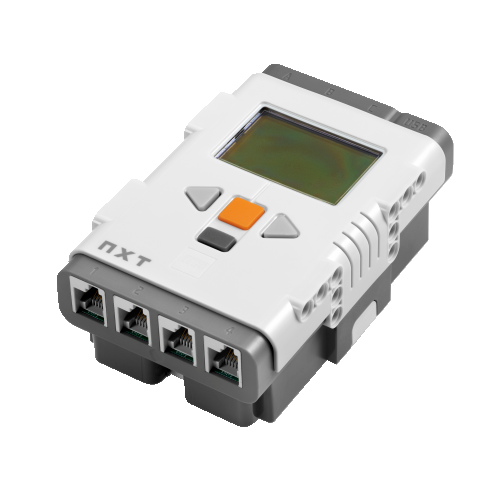
\includegraphics[scale=.5]{./graphics/nxt/brick}
\end{center}
\caption{NXT Intelligent Brick.}
\label{platform:nxt}
\end{figure}

\subsubsection{Porte}
NXTen har 3 motorporte (kaldet A, B og C) og 4 sensorporte (kaldet 1, 2, 3 og 4).

\subsubsection{Tilslutningsmuligheder}
Der kan kommunikeres med NXTen ved at tilslutte den til en anden enhed med USB-kabel eller Bluetooth.

\subsubsection{Feedback}
Til output har NXTen en 100 x 64 pixel LCD display, samt en 8 kHz højttaler.

\subsubsection{Styring}
NXTen kan styres på to måder:
Man kan sende kommandoer og modtage beskeder (for eksempel sensor aflæsninger) på en ekstern enhed (oftest en computer eller en anden NXT).
Alternativt kan programmer sendes (via Bluetooth eller USB) til NXTen, hvorfra de kan køres direkte, uafhængig af eksterne enheder.


\subsubsection{Tekniske specifikationer}
De tekniske specifikationer for NXT 2.0 kan ses i \cref{mindstorms:tekniske_spec} \cite{nxt}. 


\begin{table}[h]
\begin{tabular}{|c |c|}
\hline
Microcontroller & \shortstack{\\32-bit ARM7 microcontroller\\ 8-bit AVR controller}\\
\hline
RAM & \shortstack{ \\256 Kb FLASH, 64 Kb RAM \\ 4 Kb FLASH, 512 b RAM} \\
\hline
Kommuniation & \shortstack{ \\Bluetooth (Bluetooth Class II V2.0 compliant) \\ USB full speed port (12 Mbit/s)}\\
\hline
Input porte & 4 \\
\hline
Output porte & 3 \\
\hline
Display & 100 x 64 pixel LCD \\
\hline
Højttaler & 8 kHz lyd. 8-bit lydkanal og 2-16 kHz sample rate\\
\hline
Strømkilde & 6 AA batteries\\
\hline
\end{tabular}
\caption{\legoms NXT tekniske specifikationer.}
\label{mindstorms:tekniske_spec}
\end{table}


\subsection{Valg af \legoms}
Der er mange gode grunde til at vælge \legoms.
Her er givet fire overordnede punkter, der efterfølgende vil blive gennemgået:

\begin{itemize}
\item{Tilgængelighed}
\item{Nemt at gå til}
\item{Stort udvalg af sensorer}
\item{Mange muligheder ift. styring}
\end{itemize}

\subsubsection{Tilgængelighed}
Grundet at \lego (inkl. \legoms) er ment til almindelige brugere, er det masseproduceret og derved kan købes forholdsvist billigt og i helt almindelige butikker (legetøjsforretninger og ofte også supermarkeder).

\subsubsection{Nemt at gå til}
Det faktum at man bygger sin robot i \lego klodser, med tilføjelse af \legoms sensorer/aktautorer gør det nemt at lave en konstruktion og derefter modificere den, så den udfører sin opgave tilfredsstillende.

Denne høje alsidighed gør, at \lego er perfekt til en prototype-orienteret fremgangsmåde for bygning af robotter.

\subsubsection{Stort udvalg af sensorer}
På grund af det store udvalg af sensorer, kan man bygge robotter der kan løse et væld af opgaver.
Ved et projekt med høj usikkerhed, er det derved også nemt og billigt at udskifte en sensor, hvis den ikke virker tilfredsstillende.

\subsubsection{Mange muligheder ift. styring}
Fleksibiliteten i forhold til styring er ment både som den overordnet  måde hvorpå robotten styres, men især også den måde hvorpå NXT'en styres.
NXT'en kan udstyres med brugerdefineret firmware, der kan tilføje ekstra funktionalitet i forhold til \legos egen.

I afsnittet herefter vil der blive argumenteret for valg af API, hvor API her skal forstås som måden hvorpå robotten skal styres.

\section{NXT API}\label{nxt_api}
Den ideelle løsning ville være at vælge et system, hvor robotten styrer alt; navigation og indsamling af sensormålinger, samt selve kortlægningsdelen.
Dog er der begrænset med plads til data på NXT'en, samtidig med at den er begrænset af dens regnekraft (se evt. \cref{mindstorms:tekniske_spec}).
På grund af robottens hardwaremæssige begrænsninger og at problemformuleringen siger, at robotten til enhver tid skal kende sin position, er det derfor nødvendigt at 'outsource' visse opgaver til en PC.
Dette ses blandt andet ved, at der benyttes en Microsoft Kinect til at lokalisere robotten, hvilket gør en PC påkrævet for at bearbejde billeddata fra Kinecten, for netop at fortælle robotten dens faktiske position.

Grundet disse begrænsninger og givet problemet der skal løses, er det muligt at lave et to-delt system.
Den ene del bestående af selve robotten, som skal navigere sig rundt i verden og bruge sine sensorer til at opfatte verden omkring sig.
Den anden del, som består af selve kortlægningen, kræver mere plads til data, samt større beregningskraft.

\subsubsection*{Overordnet valg}
For at overholde ovenstående, skal der laves et to-delt stykke software, hvor den ene del kører på robotten og den anden del på en stærkere platform, i vores tilfælde en PC.

Dernæst vælges hvordan det software, der skal køre på henholdsvis robotten og på PC'en skal laves.
Vigtigt er, at det skal være muligt for de to enheder at kommunikere, da der skal kunne sendes kommandoer til robotten fra PC'en, samt at PC'en skal kunne modtage sensormålinger fra robotten.

\subsubsection*{NXC}
Til det software, der skal køre på robotten, har vi valgt NXC, da det er simpelt og dækker alle behov.
NXC-programmer skrives i et C-lignende sprog, som kan sendes til NXT'en og køres direkte der på.
Der er også stor mulighed for kommunikation mellem NXC-programmer og eksterne programmer.
Dette gør det muligt at skrive et program til NXT'en, hvorefter der kan udføres forskellige handlinger, afhængig af hvad PC'en beder den om.
Der vil blive gået mere i dybden med NXC i \cref{nxc}.

\subsubsection*{MindSqualls}
Til det software, der skal køres på PC, altså det der skal sørge for selve opdateringen og beregningen af kort, har vi valgt \mindsqualls.
\mindsqualls er et .NET bibliotek skrevet i \csharp, hvori det er muligt at kommunikere med en NXT, både ved at sende direkte kommandoer eller via abstraktion over NXT'ens aktuatorer/sensorer opfattet som objekter.
Valget faldt på \mindsqualls da dette var simpelt og dækkede alle behov ift. kommunikation med NXT.
Desuden har gruppen stor erfaring med \csharp og Visual Studio, hvilket også ses som en stor fordel.
\mindsqualls vil blive uddybet i \cref{mindsqualls}.

Dette kapitel beskriver de frameworks der er valgt til sidst er der en begrundelse for valget.

\section{MindSqualls}\label{mindsqualls}
\mindsqualls er et .NET bibliotek til \legos NXT robotter.
\mindsqualls tillader kommunikation med NXT enheder via. Bluetooth og USB og fungerer ved at sende og modtager beskeder over disse to teknologier.
Biblioteket er skrevet i \csharp og kan dermed anvendes af alle de .NET kompatible sprog.

I det følgende afsnit gives en beskrivelse af bibliotekets struktur samt eksempler på anvendelse.

\paragraph{Abstraktion}
For at gøre det nemt at arbejde med NXT motorer og sensorer er der i \mindsqualls lavet en abstraktion over disse.
Hver type I/O er således implementeret i hver sin klasse med passende funktioner.
\Cref{mindsqualls:structure} viser et klassediagram, der beskriver relationerne mellem de primære klasser i \mindsqualls biblioteket.
Herunder gives en kort gennemgang af de primære klasser i \mindsqualls.

\begin{figure}
\centering
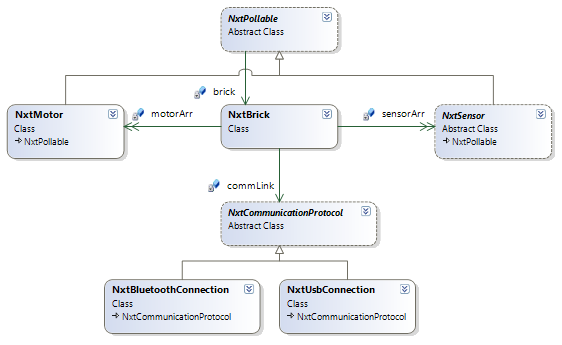
\includegraphics[width=0.8\textwidth]{mindsqualls}
\caption{Den overordnede \mindsqualls struktur}
\label{mindsqualls:structure}
\end{figure}

\subsection{NXT kommunikation}
\mindsqualls opretter forbindelse til NXT enheden vha. klassen \lstinline[style=csharp]!NxtCommunicationProtocol!.
Klassen fungerer, som navnet indikerer som en protokol ved at definere en række abstrakte funktioner.
Disse muliggører at man kan oprette forbindelse til NXT enheden, afbryde forbindelsen, og det kan til enhver tid fastslås om der er forbindelse til enheden.
Selve kommunikationen sker via kald til funktionen \lstinline[style=csharp]!Send! der tager et array af bytes som input og giver et array af bytes som output.
Altså kan funktionen både sende og modtage beskeder til og fra enheden.
Ved at lave specialiseringer af \lstinline[style=csharp]!NxtCommunicationProtocol! klassen, der definere disse funktioner, kan der kommunikeres med NXT enheden.
Der findes i \mindsqualls to specialiseringer af protokollen;
\begin{itemize}
\item \lstinline[style=csharp]!NxtUsbConnection!\\
Tillader kommunikation via USB (kablet)
\item \lstinline[style=csharp]!NxtBluetoothConnection!\\
Tillader kommunikation via Bluetooth (trådløst)
\end{itemize}

\subsection{NXT enheden}
I \mindsqualls er der lavet en abstraktion over selve NXT'en i form af klassen \lstinline[style=csharp]!NxtBrick!.
Som beskrevet herover kan der oprettes forbindelse mellem en computer og NXT enheden vha. USB eller Bluetooth.
Hvilken type forbindelse der skal benyttes angives i constructoren for \lstinline[style=csharp]!NxtBrick!.
Dette gøres med det første argument, som er en \lstinline[style=csharp]!enum! af typen \lstinline[style=csharp]!NxtCommLinkType!.
Der skal desuden angives et portnummer, som benyttes hvis der oprettes forbindelse via Bluetooth.

\begin{lstlisting}[style=csharpsmall,caption={Forbindelse til NXT enheder},label=mindsqualls:connect]
NxtBrick brickBT = new NxtBrick(NxtCommLinkType.Bluetooth, 16);
NxtBrick brickUSB = new NxtBrick(NxtCommLinkType.USB, 0);

brickBT.MotorA = ...
brickBT.Sensor1 = ...

brickBT.Connect();
// Kommunikation med enheden
brickBT.Disconnect();
\end{lstlisting}

I \cref{mindsqualls:connect} ses to eksempler på hvordan der skal oprettes forbindelse til enheden.
Selve forbindelsen oprettes ved kald til funktionen \lstinline[style=csharp]!Connect()! og afbrydes igen med \lstinline[style=csharp]!Disconnect()!.
Sensorer kan ''kobles'' til enheden ved de fire properties \lstinline[style=csharp]!Sensor1!, \lstinline[style=csharp]!Sensor2!, \lstinline[style=csharp]!Sensor3! og \lstinline[style=csharp]!Sensor4!.
Motorer anvender istedet \lstinline[style=csharp]!MotorA!, \lstinline[style=csharp]!MotorB! og \lstinline[style=csharp]!MotorC!.
Alle disse properties afspejler direkte den fysiske NXT enhed.
I \cref{mindsqualls:polling} er et eksempel på hvordan en sensor ''kobles'' til en enhed.

Når \lstinline[style=csharp]!Connect()! funktionen kaldes initialiseres enhedens tilknyttede sensorer.
Hvis man først knytter sensorer til enheden efter der er oprettet forbindelse, kaldes funktionen \lstinline[style=csharp]!InitSensors()! der sikrer at de nyligt tilknyttede sensorer er initialiserede.

\subsection{Input og Output}
For hver af de sensorer og motorer \lego producerer findes der i \mindsqualls en tilsvarende sensor.
Disse arver alle fra klassen \lstinline[style=csharp]!NxtPollable! der definerer metoder til at læse værdier fra de forskellige komponenter.
Dette gøres ved et \emph{Poll} der opdaterer den enkelte klasses tilstand således at den svarer til det fysiske komponent.
Samtidig er der for \lstinline[style=csharp]!NxtPollable! implementeret parallel automatisk polling.
Altså er det muligt automatisk at opdatere et komponents status.
Brugen af polling (både manuel og automatisk) kan ses i \cref{mindsqualls:polling}.
Her ses det også at polling er implementeret med et event der smides hver gang \lstinline[style=csharp]!Poll! kaldes.
I eksemplet er eventhandleren implementeret med et lambda udtryk der udskriver tilstanden for sensoren.

\begin{lstlisting}[style=csharpsmall,caption={Et eksempel på polling i \mindsqualls},label=mindsqualls:polling]
NxtUltrasonicSensor sonar = new NxtUltrasonicSensor();

sonar.OnPolled += pollable =>
    Console.WriteLine("Distance: {0}", sonar.DistanceCm);

brick.Sensor1 = sonar;

sonar.Poll();
// eller
sonar.PollInterval = 1000;
\end{lstlisting}

\subsubsection{Brug af sensorer}
Som et eksempel på brugen af sensor-klasser betragtes \legos ultralyds sensor (\cref{sensor:ultrasonic_sensor}), som er repræsenteret ved klassen \lstinline[style=csharp]!NxtUltrasonicSensor!.
Denne har en property \lstinline[style=csharp]!DistanceCm! der, som navnet angiver, returnerer afstanden fra sensoren til det objekt der er foran den.
I \cref{mindsqualls:polling} ses et eksempel på hvordan en sådan sensor oprettes og forbindes til NXT'en.

\subsubsection{Brug af motorer}
\legoms Servo Motoren er både en aktuator og en sensor, hvorfor det er muligt både at aflæse motorens nuværende position (med position menes der ændringen i grader ift. udgangspunktet), eller at sende kommandoer til at manipulere den nuværende position.

Til at aflæse løbende opdateringen, bruges samme metode som til aflæsning af de andre sensorer, via \textit{Polling}.

De vigtigste metoder til styring af motoren kan ses i brug i \cref{mindsqualls:motor}.
Her initialiseres en ny motor, hvorefter den roterer en hel omgang (360 grader), med hastighedsniveau 50 (som går fra 0 til 127).
Hvorefter den ny position bliver aflæst og skrevet til konsollen.

\begin{lstlisting}[style=csharpsmall,caption={Et eksempel på brug af en motor i \mindsqualls},label=mindsqualls:motor]
NxtMotor motor = new NxtMotor();
brick.MotorA = motor;

motor.Run(20, 360);
motor.Brake();

Console.WriteLine("Position: {0}", motor.TachoCount ?? 0);
\end{lstlisting}

\subsubsection{Styring af motorer}
Ved at sende kommandoer til ændring af motor-tilstand direkte til NXT'en kan der være høj unøjagtighed.
Dette gælder ved rotation af en enkelt motor, dette er især et problem hvis der er to motorer der bør køre synkront.
Derfor er det nødvendigt at benytte \textit{MotorControl}.

\paragraph{MotorControl} er et program der lægges ind på NXT'en (en .rxe-fil), som kører motor kommandoerne i stedet for det normale output.
På denne måde bør der være helt ned til 1 grads unøjagtighed.

Den måde som MotorControl bruges i mindsqualls, er med et sæt nye klasser til brick og motorer: \lstinline[style=csharp]!McNxtBrick!, \lstinline[style=csharp]!McNxtMotor! og \lstinline[style=csharp]!McNxtMotorSync!.
Alternativt kan der bruges den statiske klasse \lstinline[style=csharp]!MotorControlProxy! hvor der kan kommunikeres direkte med MotorControl på NXT'en, uden lige så høj abstraktion.

\paragraph{Eksempel} på brugen af MotorControl kan ses i \cref{mindsqualls:motorcontrol}, hvor der udføres samme funktionalitet som i \cref{mindsqualls:motor}, blot med brug af MotorControl.
Yderligere aktiveres MotorControl programmet på NXT'en, hvis det ikke allerede kører.

\begin{lstlisting}[style=csharpsmall,caption={Et eksempel på brug af MotorControl},label=mindsqualls:motorcontrol]
McNxtMotor mcMotorA = new McNxtMotor();

mcBrick.MotorA = mcMotorA;

if (!mcBrick.IsMotorControlRunning())
    mcBrick.StartMotorControl();

mcMotorA.Run(20, 360);

Console.WriteLine("Position: {0}", mcMotorA.TachoCount ?? 0);
\end{lstlisting}


\subsection{NXC}\label{nxc}
Til at programmere robotten (NXTen) har vi valgt at benytte NXC; et programmeringssprog designet til NXT robotten. 
Brugen af NXC til at styre robotten vil blive beskrevet her.\cite{NXC}
Desuden bruges Enhanced Firmware, for at få adgang til trigonometriske funktioner, som er nødvendige for projektet.\cite{enhanced_firmware}

\subsubsection{NXC sproget}
NXC har en syntax der minder meget om C syntax. 
Ud over de traditionelle programmeringskonstruktioner indeholder NXC en masse standardfunktioner til at interagere med robottens sensorer og motorer.

\subsubsection{Sensorer og motorer}
NXC sproget indeholder funktioner til at styre sensorer og motorer tilsluttet NXTen.
Et eksempel på aktivering af en sensor og en motor kan ses i \cref{nxc:sensors}.
\lstinline[style=c]!SetSensor! bruges først til at fortælle robotten at indgang 1 er en touch sensor. 
Sensorens værdi aflæses i linje 5 fra en variabel tilknyttet porten.
Motorne i port A og C instrueres til at køre med 75 \% hastighed i linje 4 med \lstinline[style=c]!OnFwd!.  
Der findes tilsvarende en \lstinline[style=c]!OnRev! til at køre baglæns.
Motoren kører indtil der trykkes på touch sensoren, hvorefter \lstinline[style=c]!Off! kaldes for at standse motorerne.

\begin{lstlisting}[style=c,label=nxc:sensors, caption={Brug af motorer og sensorer.}]
task main()
{
 SetSensor(IN_1,SENSOR_TOUCH);
 OnFwd(OUT_AC, 75);
 until (SENSOR_1 == 1);
 Off(OUT_AC);
}
\end{lstlisting}

\subsubsection{Tasks}
\mikael{Så vidt jeg ved bruger vi ikke dette, så mon ikke bare det bør undlades?}
\bruno{enig med mikael}
Til at udnytte at NXT robotten understøtter multithreading, findes der i NXC et \lstinline[style=c]!task! keyword.
Et NXC program består af maksimalt 255 tasks, der hver har et unikt navn. 
Der skal altid findes en \lstinline[style=c]!Main! task, da denne køres først.
Main task'en skal terminere før andre tasks kan køres, og tasks skal enten køres eksplicit eller planlægges (schedules).

Tasks kan schedules på en af følgende måder:

\begin{description}
\item{\lstinline[style=c]!Precedes(task1,task2,...,taskN!)}

Erklærer at denne task kommer før de angivne tasks. 
De angivne tasks vil blive sat til at køre samtidigt, når den nuværende task afsluttes.
\item{\lstinline[style=c]!Follows(task1,task2,...,taskN!)}

Erklærer at denne task kommer efter de angivne tasks. 
De angivne tasks skal afsluttes før den nuværende task får lov til at køre.
\end{description}

Tasks kan startes og stoppes med de følgende kommandoer:

\begin{description}
\item{\lstinline[style=c]!StartTask(task t)!}

Starter den angivne task

\item{\lstinline[style=c]!StopTask(task t)!}

Stopper den angivne task
\end{description}

Der er i sproget indbygget en \lstinline[style=c]!mutex! datatype til brug ved samtidig programmering, samt en \lstinline[style=c]!Acquire! og en \lstinline[style=c]!Release! funktion.
Et eksempel på brug af mutex kan ses i \cref{nxc:mutex}

\begin{lstlisting}[style=c,label=nxc:mutex, caption={Eksempel på brug af mutex.}]
mutex moveMutex;

task move_square()
{
  while (true)
    {
      Acquire(moveMutex);
      OnFwd(OUT_AC, 75); Wait(1000);
      OnRev(OUT_C, 75); Wait(500);
      Release(moveMutex);
    }
}

task check_sensors()
{
  while (true)
  {
    if (SENSOR_1 == 1)
    {
      Acquire(moveMutex);
      OnRev(OUT_AC, 75); Wait(500);
      OnFwd(OUT_A, 75); Wait(500);
      Release(moveMutex);
    }
  }
}

task main()
{
  Precedes(move_square, check_sensors);
  SetSensorTouch(IN_1);
}
\end{lstlisting}

\subsubsection{Kommunikation med PC}
Da der skal bruges en ekstern enhed (en PC) til visse dele af systemet, er det nødvendigt at kunne kommunikere med en PC fra NXTen.
Til kommunikation via Bluetooth findes der på NXT et antal mailboxe.
Disse anvendes til at sende og modtage beskeder.
Et eksempel på at modtage en besked kan ses i \cref{nxc:receive}.
\lstinline[style=c]|ReceiveRemoteString| bruges til at kigge om der er en ny besked i \lstinline[style=c]!INBOX!.
Denne bliver fjernet fra inboxen, hvis det andet parameter er \lstinline[style=c]|true|, og beskeden bliver læst over i strengen \lstinline[style=c]|in|.

\begin{lstlisting}[style=c,label=nxc:receive,caption={Et eksempel på at modtage beskeder over Bluetooth.}]
#define INBOX 5
#define OUTBOX 6

while(true){
  ReceiveRemoteString(INBOX,true,in)
  
  if(StrLen(in) > 0)
  {
    tmp = SubStr(in,0,1);
    packet = StrToNum(tmp);
    PlayToneEx(100* packet, 200, 3,false);
  }
  in = "";
}
\end{lstlisting}

I \cref{nxc:receive-mindsqualls} er den tilhørende kode i \mindsqualls, der afsender en besked.
Først gemmes beskeden i en streng og derefter afsendes beskeden via \lstinline[style=csharp]!NxtCommunicationProtocol! klassens \lstinline[style=csharp]!MessageWrite! funktion.

\begin{lstlisting}[style=c,breaklines=true, label=nxc:receive-mindsqualls,caption={\mindsqualls kode der afsender en besked.}]
private const NxtMailbox2 PC_INBOX = NxtMailbox2.Box6;
private const NxtMailbox PC_OUTBOX = NxtMailbox.Box5;

public static void NxtTone(NxtCommunicationProtocol commLink, int tone)
{
  string messageData = string.Format("{0}", (byte)tone);
  commLink.MessageWrite(PC_OUTBOX, messageData);
}
\end{lstlisting}

Afsending af beskeder virker tilsvarende ved brug af kommandoen \lstinline[style=c]|SendMessage|.
Et eksempel på at afsende en besked kan ses i \cref{nxc:send}.
\lstinline[style=c]|SendMessage| benyttes til at sende beskeden \lstinline[style=c]|msg| til \lstinline[style=c]!OUTBOX!.

\begin{lstlisting}[style=c,label=nxc:send,caption={Eksempel på afsending af besked.}]
while(true){
  string msg = NumToStr(SENSOR_1);
  SendMessage(OUTBOX, msg);
}
\end{lstlisting}

I \cref{nxc:send-mindsqualls} ses den tilhørende \mindsqualls kode, der læser en besked sendt fra NXTen.

\begin{lstlisting}[style=c,breaklines=true,label=nxc:send-mindsqualls,caption={\mindsqualls kode der læser en besked sendt fra NXT'en.}]
public static string NxtSensorReading(NxtCommunicationProtocol commLink)
{
  return commLink.MessageRead(PC_INBOX, NxtMailbox.Box0, true);
}
\end{lstlisting}

\chapter{Sensorer og Motorer}\label{valg:sensorer}
% !TeX spellcheck = da_DK
\label{sensorer}
Følgende afsnit undersøger de tilgængelige sensorer og motorer, som er interessante for projektet.
Da der er stor forskel på sensorerne, der er til rådighed, er der foretaget forskellige forsøg, hvis formål er at klarlægge præcisionen af de forskellige sensorer.

\begin{figure}[h]
\centering
\begin{subfigure}[b]{.4\textwidth}
\centering
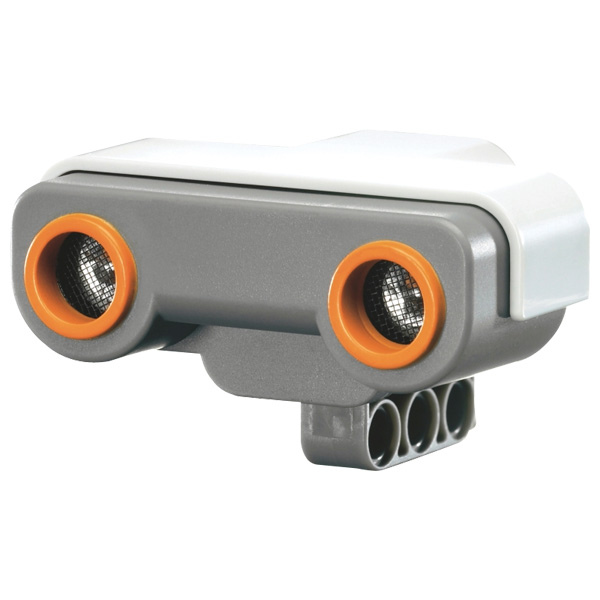
\includegraphics[width=.5\textwidth]{us}
\caption{Ultrasonisk sensor}
\label{sensor:ultrasonic_sensor}
\end{subfigure}
\begin{subfigure}[b]{.4\textwidth}
\centering
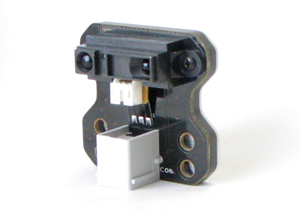
\includegraphics[width=.5\textwidth]{infrared_sensor}
\caption{Infrarød sensor}
\label{sensor:infraroed_sensor}
\end{subfigure}
\begin{subfigure}[b]{.4\textwidth}
\centering
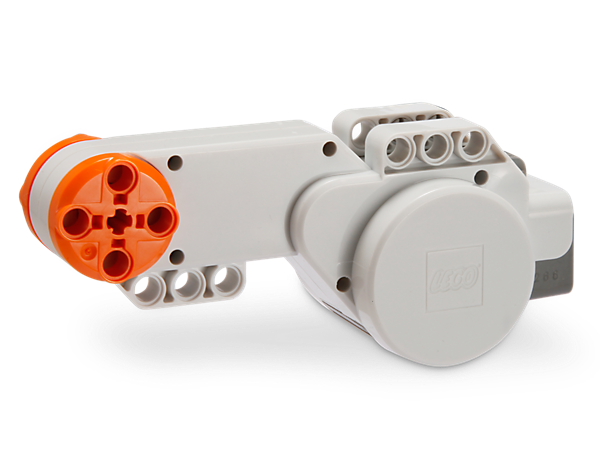
\includegraphics[width=.5\textwidth]{lego_motor}
\caption{Servomotor}
\label{sensor:servo_motor}
\end{subfigure}
\begin{subfigure}[b]{.4\textwidth}
\centering
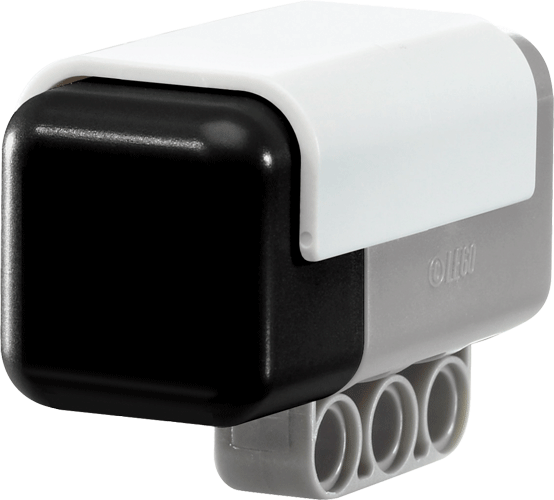
\includegraphics[width=.5\textwidth]{hitechnic_compass}
\caption{Kompas}
\label{sensor:compass}
\end{subfigure}
\caption{Komponenter der betragtes til konstruktion af robotten.}
\end{figure}

\section{Afstandssensorer}
\mikael{I kompas konkluderer vi at det ikke kunne bruges. Vi konkluderer ikke noget for hverken afstandssensor eller motor, bør vi ikke det?}
\bruno{uenig - konklusion for aftstandssensorer er at finde under sammenligning af afstandssensorer. Med motor er der ikke så mange alternativer så de rbeskriver vi bare usikkerheden.}
Dette afsnit beskriver testen af de to afstandssensorer (\cref{sensor:ultrasonic_sensor,sensor:infraroed_sensor}), som kan være interessante at montere på robotten.
For at afgøre hvilken der passer bedst til at løse problemet, er de blevet testet.

Formålet med at teste disse sensorer er, at robotten skal have en måde at afgøre på, hvor langt der er til objekter omkring den.
Derfor vil disse tests undersøge følgende:
\begin{itemize}
\item Hvor nøjagtigt kan sensorerne bestemme afstanden til et objekt?
\item Hvilket interval kan der måles i (hvad er den minimale og maksimale måleafstand)?
\end{itemize}

\subsection{Ultrasonisk Sensor} \label{subsection:ultrasonic}
Den ultrasoniske sensor, som kan ses på \cref{sensor:ultrasonic_sensor}, kan måle afstand til objekter.

Det gøres ved at sende en lydbølge, hvorefter der beregnes hvor lang tid det tager for denne at ramme objektet, for derefter at blive reflekteret tilbage igen.
Den maksimale afstand der kan måles er 255 cm, med en præcision på $\pm 3$ centimeter.
De bedste aflæsninger fåes ved måling af store flade objekter med hård overflade, i modsætning til mindre objekter med rund og/eller blød overflade.\cite{nxt}

\subsubsection{Test}
Der er gennemført en mindre test af sensoren, for at finde ud af hvor nøjagtig den er.

Testen blev udført ved at lave en simpel \lego konstruktion, kun bestående af NXT og den ultrasoniske sensor.
Konstruktionen blev placeret i en bestemt afstand fra en væg, hvor sensoreren var placeret vandret, pegende direkte på væggen.
Herefter blev sensoren aflæst, samtidig med at afstanden mellem væg og sensor blev målt med lineal.
Der blev udført den samme test 3 gange, hver gang for en bestemt række afstande mellem 0 og 255 cm.

\subsubsection{Resultater}\label{sensorer:us:resultater} Tabel med resultater fra forsøget kan ses i \cref{appendix:ultrasonisk}.

En graf-repræsentation af resultaterne kan ses i \cref{sensor:ultrasonic_resultat_diagram}.
Den røde linje indikerer det ideele resultat. mens den brune, grønne og lilla linje viser resultaterne fra de tre test.
Det ses på grafen, at de tre test alle giver forkerte resultater, når sensoren er mindre en 20 cm fra objektet.
Desuden kan det ses, at der i test 1 (brun) kun kunne måles op til 170 cm, før der opstod usikkerhed, hvor de andre tests nåede 200 cm (test 2 -- grøn) og 230 cm (test 3 -- lilla) før der opstod større usikkerhed.
Generelt overholder sensoren dens specifikationer, idet der er en afvigelse på 3 cm på målingerne, men forsøget viser, at der kun kan måles mellem 20 og 170 cm, uden der opstår større usikkerheder.

\begin{figure}[h]
\centering
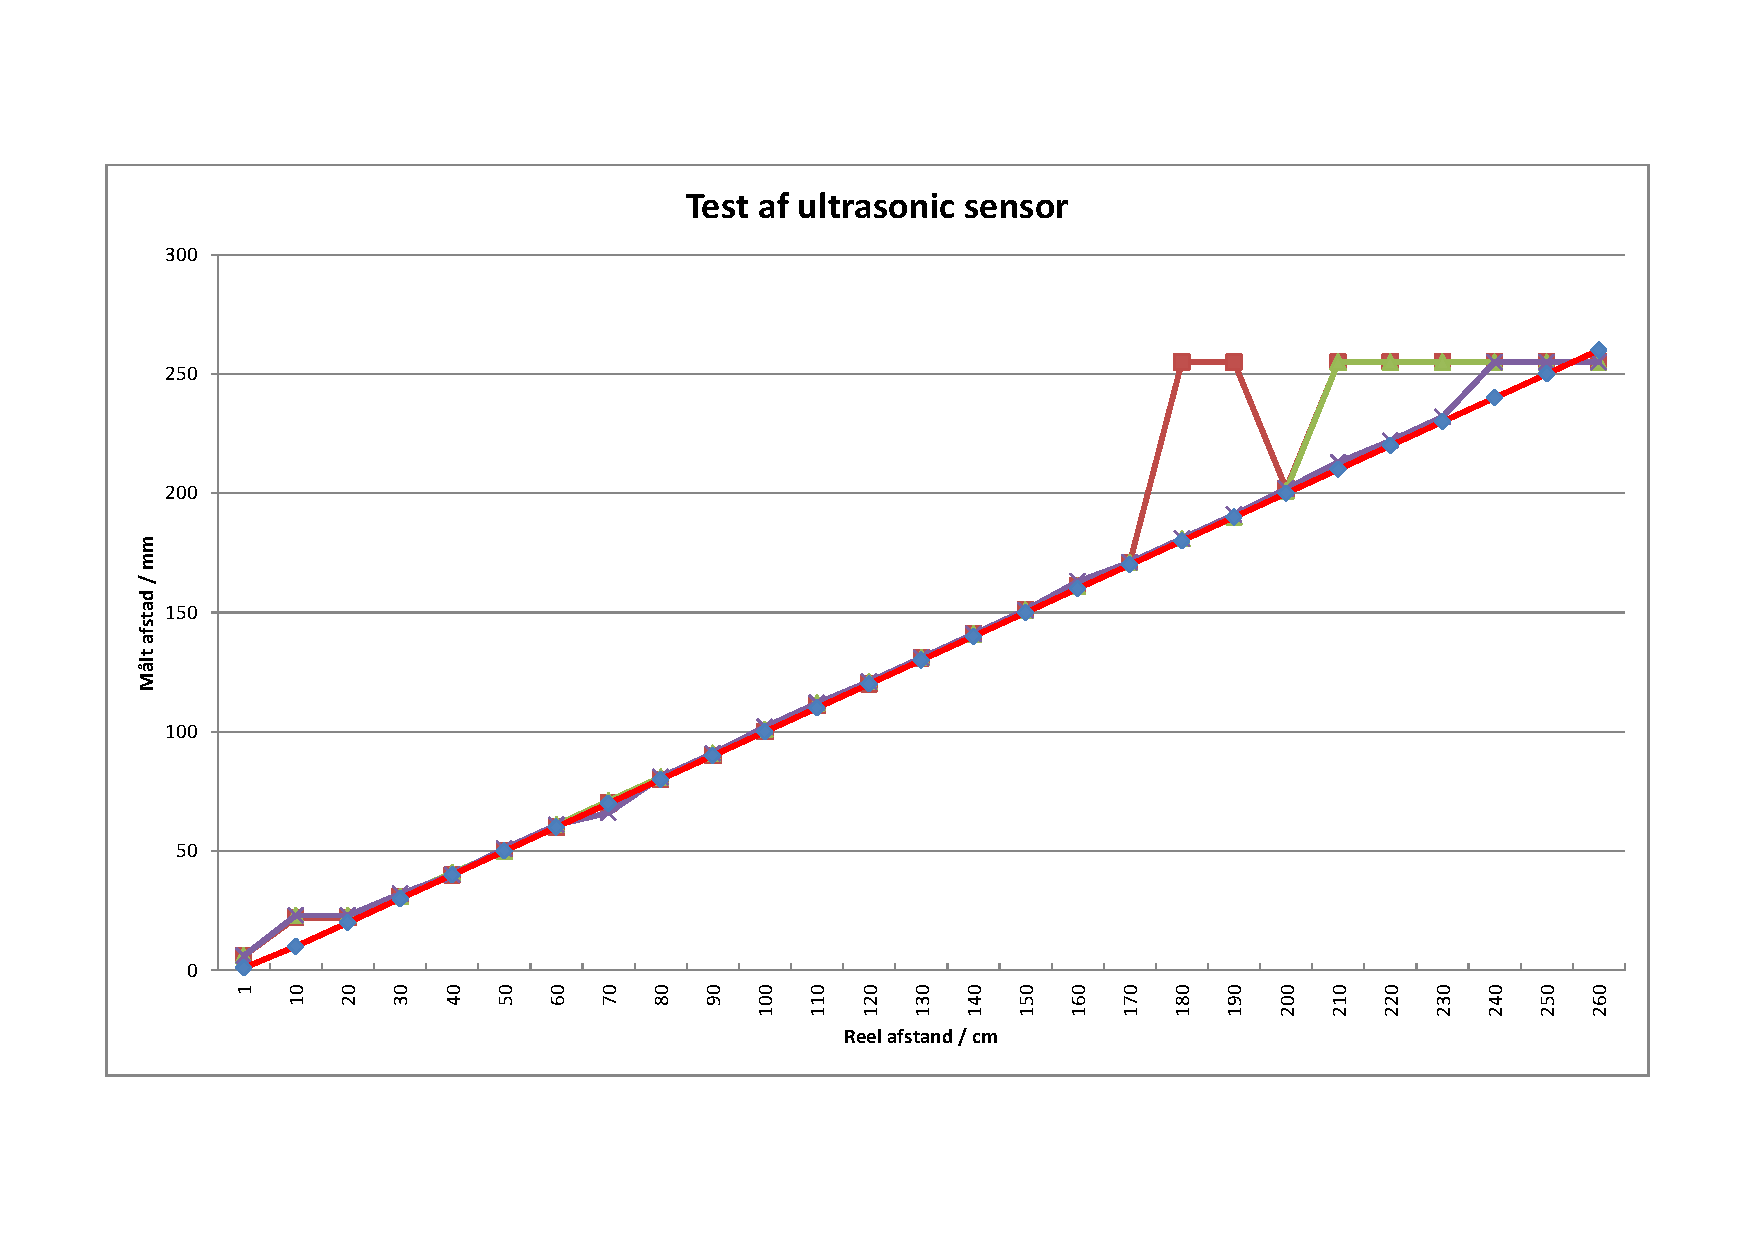
\includegraphics[clip=true, trim = 0cm 2.5cm 0cm 2.5cm,width=\textwidth]{ultrasonicchart}
\caption{Graf over forsøgsresultaterne fra testen af den ultrasoniske sensor.}
\label{sensor:ultrasonic_resultat_diagram}
\end{figure}



\subsection{Infrarød Sensor}
Den infrarøde afstandssensor fra mindsensors.com, som kan ses på \cref{sensor:infraroed_sensor}, er en afstandssensor med høj præcision, der kan måle afstande mellem 10 og 80 cm.
Sensoren virker som den ultrasoniske sensor, men sender et infrarødt lys i stedet for en ultrasonisk impuls.

\subsubsection{Test}
For at afprøve sensorens præcision og rækkevidde, er der foretaget en test af sensoren.

Opstillingen brugt til udførelse af testen bestod af tre A4 ark spændt ud på gulvet ind til en væg. 
Papiret havde markeringer for hver 2 cm fra væggen.

Udførelsen af testen gik ud på at placere en NXT med påsat infrarød sensor ved hver indikator, for derefter at aflæse sensorens måling.
På denne måde blev afmålingen fra sensoren ved en given afstand holdt op imod den egentlige afstand til væggen, som afmålt på papiret.

\subsubsection{Resultater}

Resultaterne fra testen er præsenteret i \cref{appendix:infrared}. 
Disse resultater er vist på \cref{sensor:infrared_chart}.
Den røde graf er den reelle afstand, som aflæst på papiret/med lineal, mens de blå firkanter er målepunkter.
Den sorte graf er en lineær regression over måleresultaterne.

Ud fra grafen ses det, at der er stor usikkerhed i starten og slutningen, hvilket næsten stemmer overens med den lovede rækkevidde på 10 til 80 cm.
De bedste resultater findes dog imellem 8cm og 56 cm. 
Mellem 8cm og 56cm er der maximalt 27 mm afvigelse fra det forventede, (forventet 500, målt 527).

\begin{figure}[h]
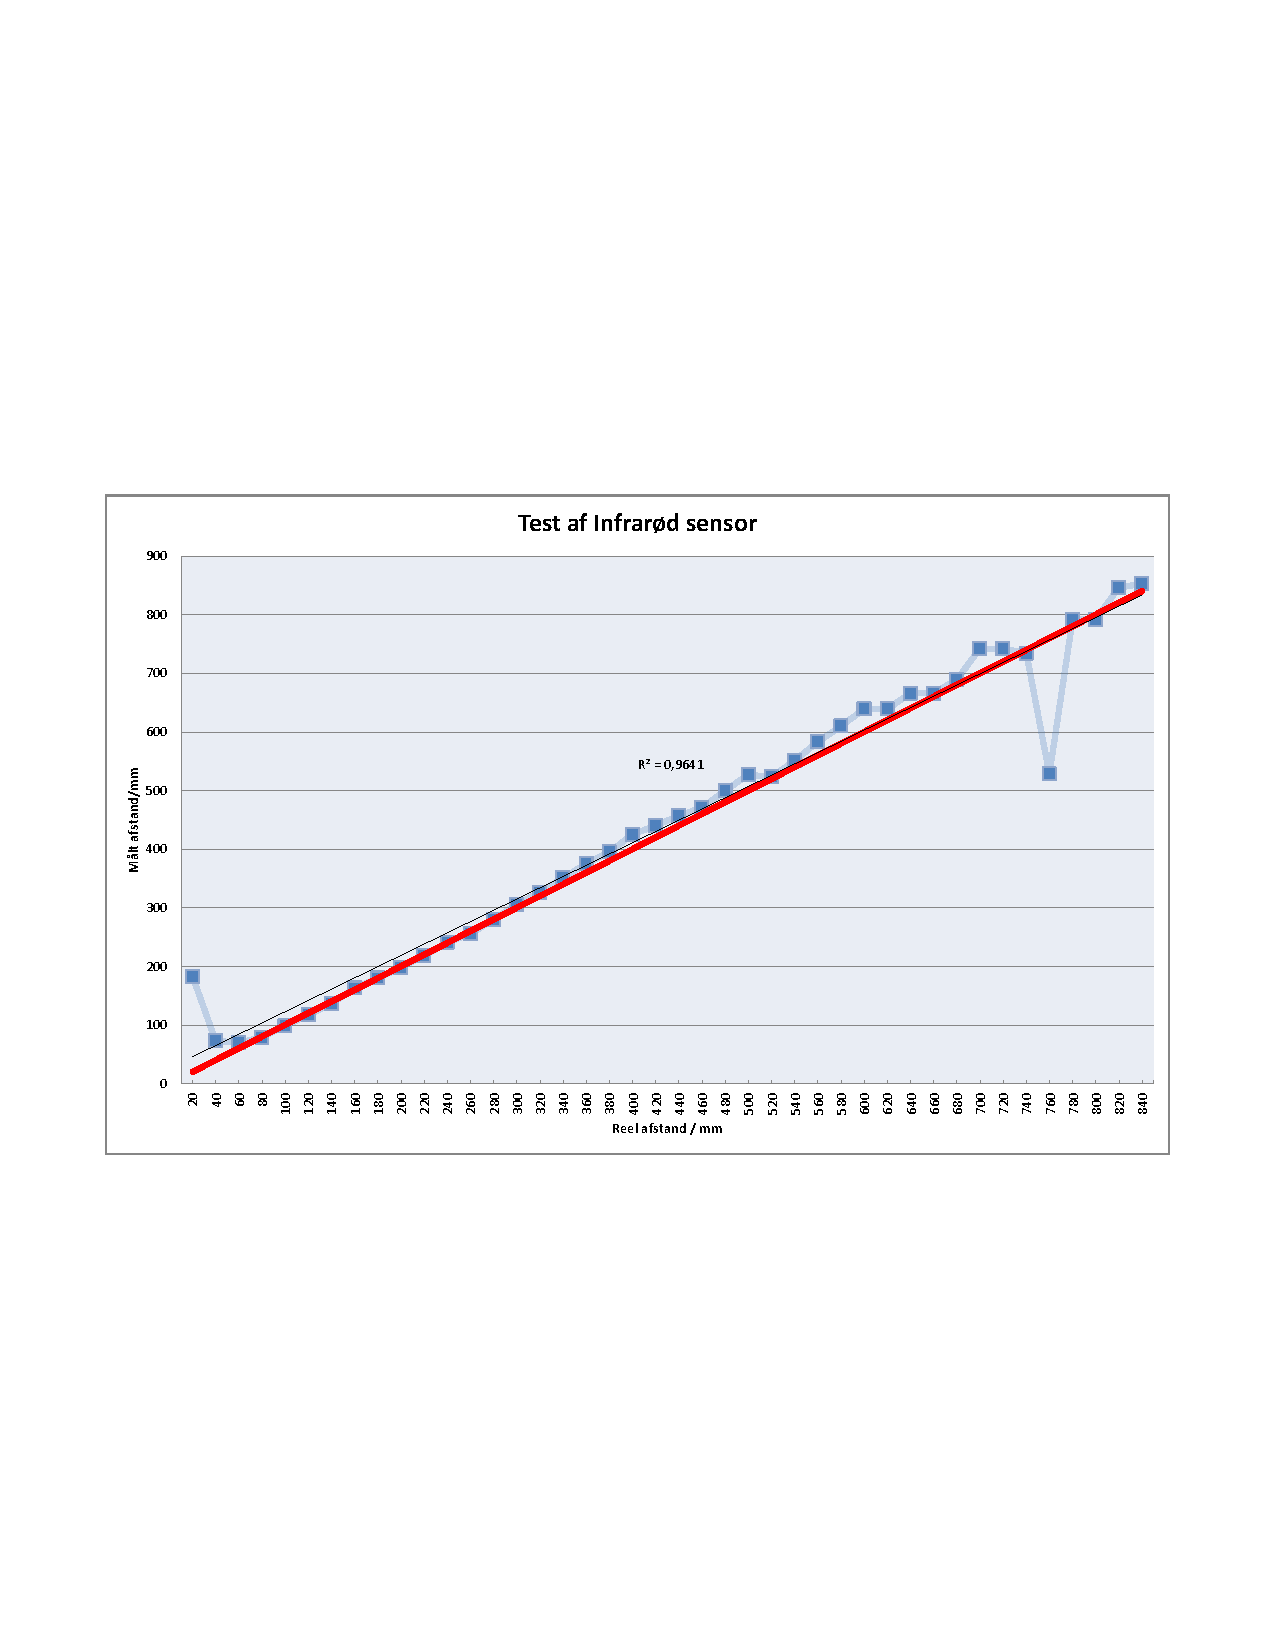
\includegraphics[clip=true, trim=0cm 8cm 0cm 8cm,width=\textwidth]{Infraredchart}
\caption{Graf over forsøgsresultaterne fra testen af den infrarøde sensor.}
\label{sensor:infrared_chart}
\end{figure}

\subsection{Sammenligning af afstandssensorer}\label{sensor:sammenligningIRvsSonar}

Der er foretaget test af to forskellige afstandssensorer, den ultrasoniske sensor og den infrarøde sensor. 
Den ultrasoniske sensor var præcis med en afvigelse på $\pm$3 cm mellem 20 cm og 170 cm.
Den infrarøde sensor var præcis med afvigelse på $\pm$3 cm, mellem 10 cm og 56 cm.
Den infrarøde sensor angiver sine målinger med højere præcision, men da fejlmarginen er 3 cm, anses den ikke som værende mere præcis end den ultrasoniske sensor.

Med en fejlmargin på 3cm, i de respektive intervaller, anses begge afstandssensorer for at være præcise nok til anvendelse i projektet.
I forhold til rækkevidde er den ultrasoniske sensor den mest \textit{præcise} af de to på større afstand, mens den infrarøde sensor er den mest \textit{præcise} på kort afstand.
Valget mellem de to sensorer er derfor afhængig af hvilket krav robotten har til rækkevidde.

\section{Motor}\label{sensorer:motorer}
Motoren, der er testet her, er fremstillet af \lego og kan ses i \cref{sensor:servo_motor}.
Den består af en rotationssensor, som måler omdrejningerne ved grader, med en nøjagtighed på \'en grad i følge \lego. 
Desuden gør denne sensor det også muligt at styre hvor meget kraft motoren skal køre med.
Køres der med flere motorer har NXTen indbygget software, der gør det muligt at synkronisere disse, hvilket er hensigtsmæssig hvis fx. den ene motor skulle være stærkere eller svagere end den anden.\cite{tikNXT}

\subsection{Formål}
Formålet med denne test er at teste motorens nøjagtighed.
Hvis motoren ikke har høj nøjagtighed, skal der tages højde for det, når den monteres på robotten.

\subsection{Test}
For at bestemme motorens nøjagtighed i praksis, blev en test opstillet hvor to moterer roteres med et bestemt antal grader.
Motorernes egentlige rotation aflæses med vinkelmåler og holdes op mod den ønskede rotation, samt den rotation motorerne angiver at de har roteret.
Sidstnævnte fås ved at aflæse motorernes \lstinline[style=csharp]!TachoCount! egenskab.

\subsubsection{Resultat}
Resultaterne fra forsøget kan ses i \cref{appendix:motor_test}. 
Af resultaterne kan vi bestemme de største afvigelser til +7 og -4 grader.
Tacho-værdien har en afvigelse på maksimalt +1 og -4 grad.
Dette stemmer ikke overens med de antagede $\pm$1 grads afvigelse.

+7 og +6 grader målt optræder kun \'en gang.
Ellers er den maksimale målte afvigelse $\pm$4 grader, men selvom vi antager, at det er pga. unøjagtige målinger ved forsøgsudførelsen, er det stadig ikke $\pm$1 grad.

Af \cref{sensor:motor_sensor_diagram} ses det at målingerne ligger længst udenfor det optimale (sorte stiplede linje), hvilket er en god indikator for, at det er bedre at benytte tacho-værdien.

\begin{figure}
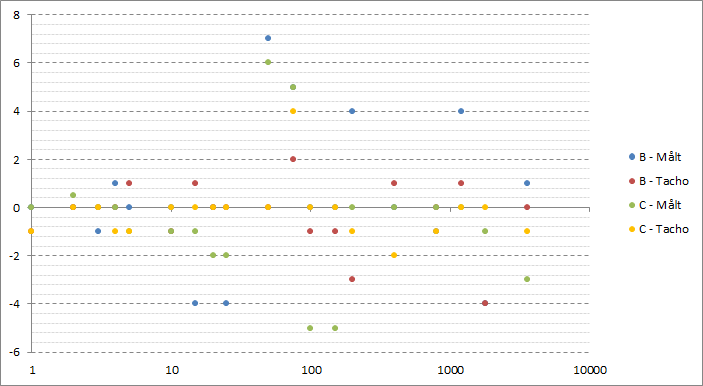
\includegraphics[width=\textwidth]{motor_diagram}
\caption{Afvigelser i test-resultaterne.}
\label{sensor:motor_sensor_diagram}
\end{figure}

Desuden kan vi se på samme figur, at motor b er meget mere unøjagtig end motor c.
Ideelt ville de to motorer give det samme resultat.

Dvs. den målte værdi har en afvigelse på $\pm$4 grader, mens tacho-værdien har en afvigelse på +1 og -4 grader, og at synkronisering af de to motorer ikke giver den ønskede effekt.

Afvigelserne i motorernes præcision er ofte ikke store, og evt. fejl vil delvist blive afhjulpet af det system der konstrueres til lokalisering af robotten.
Det vurderes derfor at præcisionen af motorerne er god nok til anvendelse i projektet.

\section{HiTechnic NXT Kompas Sensor}
Kompasset fra HiTechnic er et digitalt kompas, der måler jordens magnetiske felt.
Kompasset kan returnere en værdi, der repræsenterer kompassets nuværende orientering.
Ifølge HiTechnic er værdierne returneret fra kompasset præcise ned til 1 grad.
Kalibrering skulle desuden ikke være nødvendig.
Dog er det nødvendigt, for at minimere forstyrrelser, at kompasset holdes 10-15 cm væk fra forstyrrende elementer, herunder \lego NXT og motorer.\cite{hitechnic_compass}

I \cref{kompas:precision} undersøges hvorvidt målinger fra kompasset kan leve op til disse oplysninger.

\subsection{Formål}
Formålet med denne test er at undersøge kompassets nøjagtighed.
Hvis kompasset har høj nøjagtighed, kan det monteres på robotten og afgøre hvilken retning denne vender.

\subsection{Kompas Sensor i \mindsqualls}
Til at styre denne sensor i \mindsqualls, skal der bruges en af de seperate klasser til HiTechnic sensorerne, som findes i namespacet \lstinline[style=csharp]!NXT.MindSqualls.HiTechnic!.
Til kompas sensoren anvendes klassen \lstinline[style=csharp]!HiTechnicCompassSensor!.

\subsubsection{Aflæsning af værdier}\label{kompas:reading}
Ved aflæsning af egenskaben \lstinline[style=csharp]!Heading! fra sensores klasse, gives et heltal mellem 0 og 359, der angiver kompassets orientering.
Det har været nødvendigt at ændre implementationen af \lstinline[style=csharp]!Heading!, da den oprindelige implementation ikke aflæste kompassets orientering ned til \'en grad.
Sensoren repræsenterer sin orientering på to forskellige måder.
Begge anvender to bytes.
Den ene metode beskriver afstanden vha. et 16-bit heltal.
Den anden (som var anvendt i implementationen af \lstinline[style=csharp]!Heading!) beskriver afstanden ved at lade den ene byte angive vinklen i intervaller af to grader.
Altså kunne de værdier der aflæses fra denne byte være 0-179, hvilket efterfølgende ganges med 2 for at få den egentlige værdi.
Hertil lægges værdien af den anden byte, der kan have værdien 0 eller 1.
I den oprindelige implementation af \lstinline[style=csharp]!Heading!, er der ikke taget højde for denne ekstra værdi.
Dette er inddraget i test 3 i det følgende afsnit.

\subsection{Præcisionstest}\label{kompas:precision}
For at teste kompas sensoren, er målinger taget fra denne og holdt sammen med målinger foretaget med vinkelmåler.
Sammenligningen er sket ved at tage to målinger med kompasset og sammenligne differencen med den værdi målt med vinkelmåler.
I forbindelse med test af sensoren, blev der udført i alt tre tests:
\begin{enumerate}
\item Kompas monteret på robot med hjul
\item Kompas monteret på fast konstruktion
\item Gentagelse af test 2, med \textit{øget præcision}
\end{enumerate}
Den øgede præcision der beskrives her, dækker over en opdatering af \mindsqualls klassen \lstinline[style=csharp]!HiTechnicCompassSensor!, der blev foretaget efter de første to tests.
Resultaterne fra de tre tests kan ses i tabellerne \ref{kompas:test1:table}, \ref{kompas:test2:table} og \ref{kompas:test3:table} på side \pageref{kompas:test1:table}.

Af resultaterne er der lavet et boksplot (\cref{kompas:boksplot}).
Plottet illustrerer den afvigelse, der var fra de værdier, der blev aflæst af kompasset, til de værdier, der blev målt med vinkelmåler.
Prikkerne på plottet repræsenterer den gennemsnitlige afvigelse.

\begin{figure}[h]
\centering
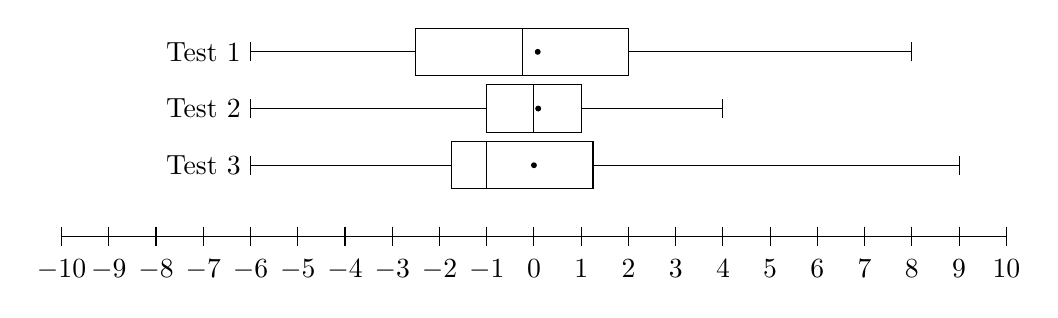
\begin{tikzpicture}[scale=0.6]
%Test 1
\draw (-2.5,3.4) rectangle (2,4.4); % Boks
\draw (-0.25,3.4) -- (-0.25,4.4); % Median streg
\draw (2,3.9) -- (8,3.9); % Fra øvre kvartil til maks
\draw (-2.5,3.9) -- (-6,3.9);% Fra nedre kvartil til min
\draw (8,3.7) -- (8,4.1); % Maksimum vertikal streg
\draw (-6,3.7) -- (-6,4.1); % Minimum vertikal streg
\node[left] at (-6,3.9) {Test 1};
\filldraw[color=black] (0.08,3.9) circle (0.05cm); % Gennemsnittet

%Test 2
\draw (-1,2.2) rectangle (1,3.2); % Boks
\draw (0,2.2) -- (0,3.2); % Median streg
\draw (1,2.7) -- (4,2.7); % Fra øvre kvartil til maks
\draw (-1,2.7) -- (-6,2.7);% Fra nedre kvartil til min
\draw (4,2.5) -- (4,2.9); % Maksimum vertikal streg
\draw (-6,2.5) -- (-6,2.9); % Minimum vertikal streg
\node[left] at (-6,2.7) {Test 2};
\filldraw[color=black] (0.09,2.7) circle (0.05cm); % Gennemsnittet

%Test 3
\draw (-1.75,1) rectangle (1.25,2); % Boks
\draw (-1,1) -- (-1,2); % Median streg
\draw (1.25,1.5) -- (9,1.5); % Fra øvre kvartil til maks
\draw (-1.75,1.5) -- (-6,1.5);% Fra nedre kvartil til min
\draw (9,1.3) -- (9,1.7); % Maksimum vertikal streg
\draw (-6,1.3) -- (-6,1.7); % Minimum vertikal streg
\node[left] at (-6,1.5) {Test 3};
\filldraw[color=black] (0.00,1.5) circle (0.05cm); % Gennemsnittet

% Linje med værdier
\draw (-10,0) -- (10,0);

% Tal på linje
\foreach \x in {-10,-9,...,10} {
	\draw (\x, 0.2) -- (\x, -0.2);
     \node[below] at (\x, -0.3) {$\x$};
}

\end{tikzpicture}
\caption{Boksplot for test af kompas.}
\label{kompas:boksplot}
\end{figure}

\subsubsection{Test 1: Monteret på robot}
Første forsøg blev udført med kompasset monteret ovenpå ultralyds-sensoren, for at holde en minimum-afstand på 15 cm fra brick og motorer.
Denne konstruktion var dog meget ustabil, da kompasset skulle være forholdsvist højt oppe ift. base-konstruktionen.

\subsubsection{Test 2: Monteret på stabil konstruktion}
Andet forsøg blev udført med kompasset monteret på en selvstændig og langt mere stabil konstruktion, for derved at undersøge om dette kunne forbedre resultaterne.

\subsubsection{Test 3: Forøget præcision (stabil konstruktion)}
Tredje forsøg var en gentagelse af det andet, efter implementationen af \lstinline[style=csharp]!Heading! blev opdateret.
Målingerne her skulle altså udtrykke en øget præcision i forhold til den forrige test.
De første to test er taget med, da forbedringen af præcisionen højst kunne være \'en grad ved denne tredje test (se \textit{\cref{kompas:reading}: \nameref*{kompas:reading}}).
Altså en marginal forbedring i forhold til testresultaterne.

\subsubsection{Resultater}
Resultaterne kan ses i \cref{appendix:kompas_test}. Som det fremgår af \cref{kompas:boksplot} er den gennemsnitlige afvigelse (prikken) i alle test meget tæt på 0.
Altså ved vi at kompasset laver lige mange og lige store (i gennemsnit) udsving til begge sider, hvilket gør det sværere at kalibrere for sådanne udsving.
Samtidig viser plottet, at halvdelen af kompassets målinger er over 2-3$\dg$ ved siden af de egentlige målinger - med den største afvigelse på 9$\dg$.

Det har i testfasen vist sig, at kompasset er konsistent i dets målinger.
Dette betyder, at der ikke kan opnås yderligere præcision ved at foretage flere målinger af samme grad.
Disse målinger vil ganske enkelt give samme resultat.

Det kan hermed konkluderes, at kompas sensoren ikke har høj nok præcision til at kunne anvendes i projektet.


\chapter{Lokalisering}\label{valg:lokalisering}
% !TeX spellcheck = da_DK
 \section{Microsoft Kinect}
En Kinect er et Natural User Interface (NUI) udviklet til Microsoft's spillekonsol, Xbox.
Den gør det muligt at interagere med sin konsol ved at bevæge kroppen og via talte kommandoer.
Den første version der udkom i november 2010~\cite{kinectWiki} er oprindeligt udviklet med henblik på at lokke nye typer brugere til Xbox med det argument at det via naturlig (og aktiv) bevægelse er sjovere og mere virkelighedstro at spille.

I februar 2012 blev der lanceret en ny type Kinect, kaldet Kinect for Windows, der sammen med et Software Development Kit (SDK), der gør det muligt at udvikle både kommercielle og non-kommercielle applikationer til Kinect der kan køres på Windows platformen.
Kort fortalt er Microsoft's Kinect mere end en input enhed gamere kan bruge for at gøre deres spiloplevelse mere virkelighedstro; af andre anvendelser kan f.eks. nævnes~\cite[s.~17]{kinectProgrammingGuide}:

\begin{itemize}
\item Optagelse af video i real-tid
\item Generere et dybde billede ved hjælp af kameraet og de to IR sensorer
\item Sende talte kommandoer
\item Vurdering af omgivelserne ved hjælp af lyd
\end{itemize}

I dette projekt skal Kinecten benyttes til at bestemme en autonom robots placering i ukendte omgivelser. 
De nævnte egenskaber ved Kinecten kan benyttes til at løse dette problem.
Derfor vil Kinecten, både med hensyn til hardware, men også til software blive nærmere beskrevet i de følgende afsnit.


\subsection{Opbygning af Kinect}
I denne rapport er det versionen Kinect for Windows der fokuseres på, da den giver bedst kompatibilitet med PC samt det faktum at den er tilgængelig gennem universitetet.

Dog kan det nævnes at forskellene mellem den og versionen til Xbox er meget små.
Hardware mæssigt har Kinect for Windows den fordel at firmwaren indeholder en såkaldt Near Mode, hvilket gør det muligt at følge objekter indtil 40 cm fra enheden.
Kinect for Xbox har ikke denne funktionalitet, og kan derfor kun følge objekter indtil 80 cm fra enheden, hvilket kan blive et problem i situationer hvor man ønsker at detektere små afstande via dybdebilleder.
Kinect for Windows kan desuden også benyttes til kommercielle applikationer, hvor dens pendant er beregnet til hobbyister, generel udvikling og forskning~\cite[s.~16]{kinectProgrammingGuide}.

For at Kinecten kan følge et objekt er Kinecten udstyret med et antal sensorer der nu vil blive beskrevet.

\begin{figure}
\centering
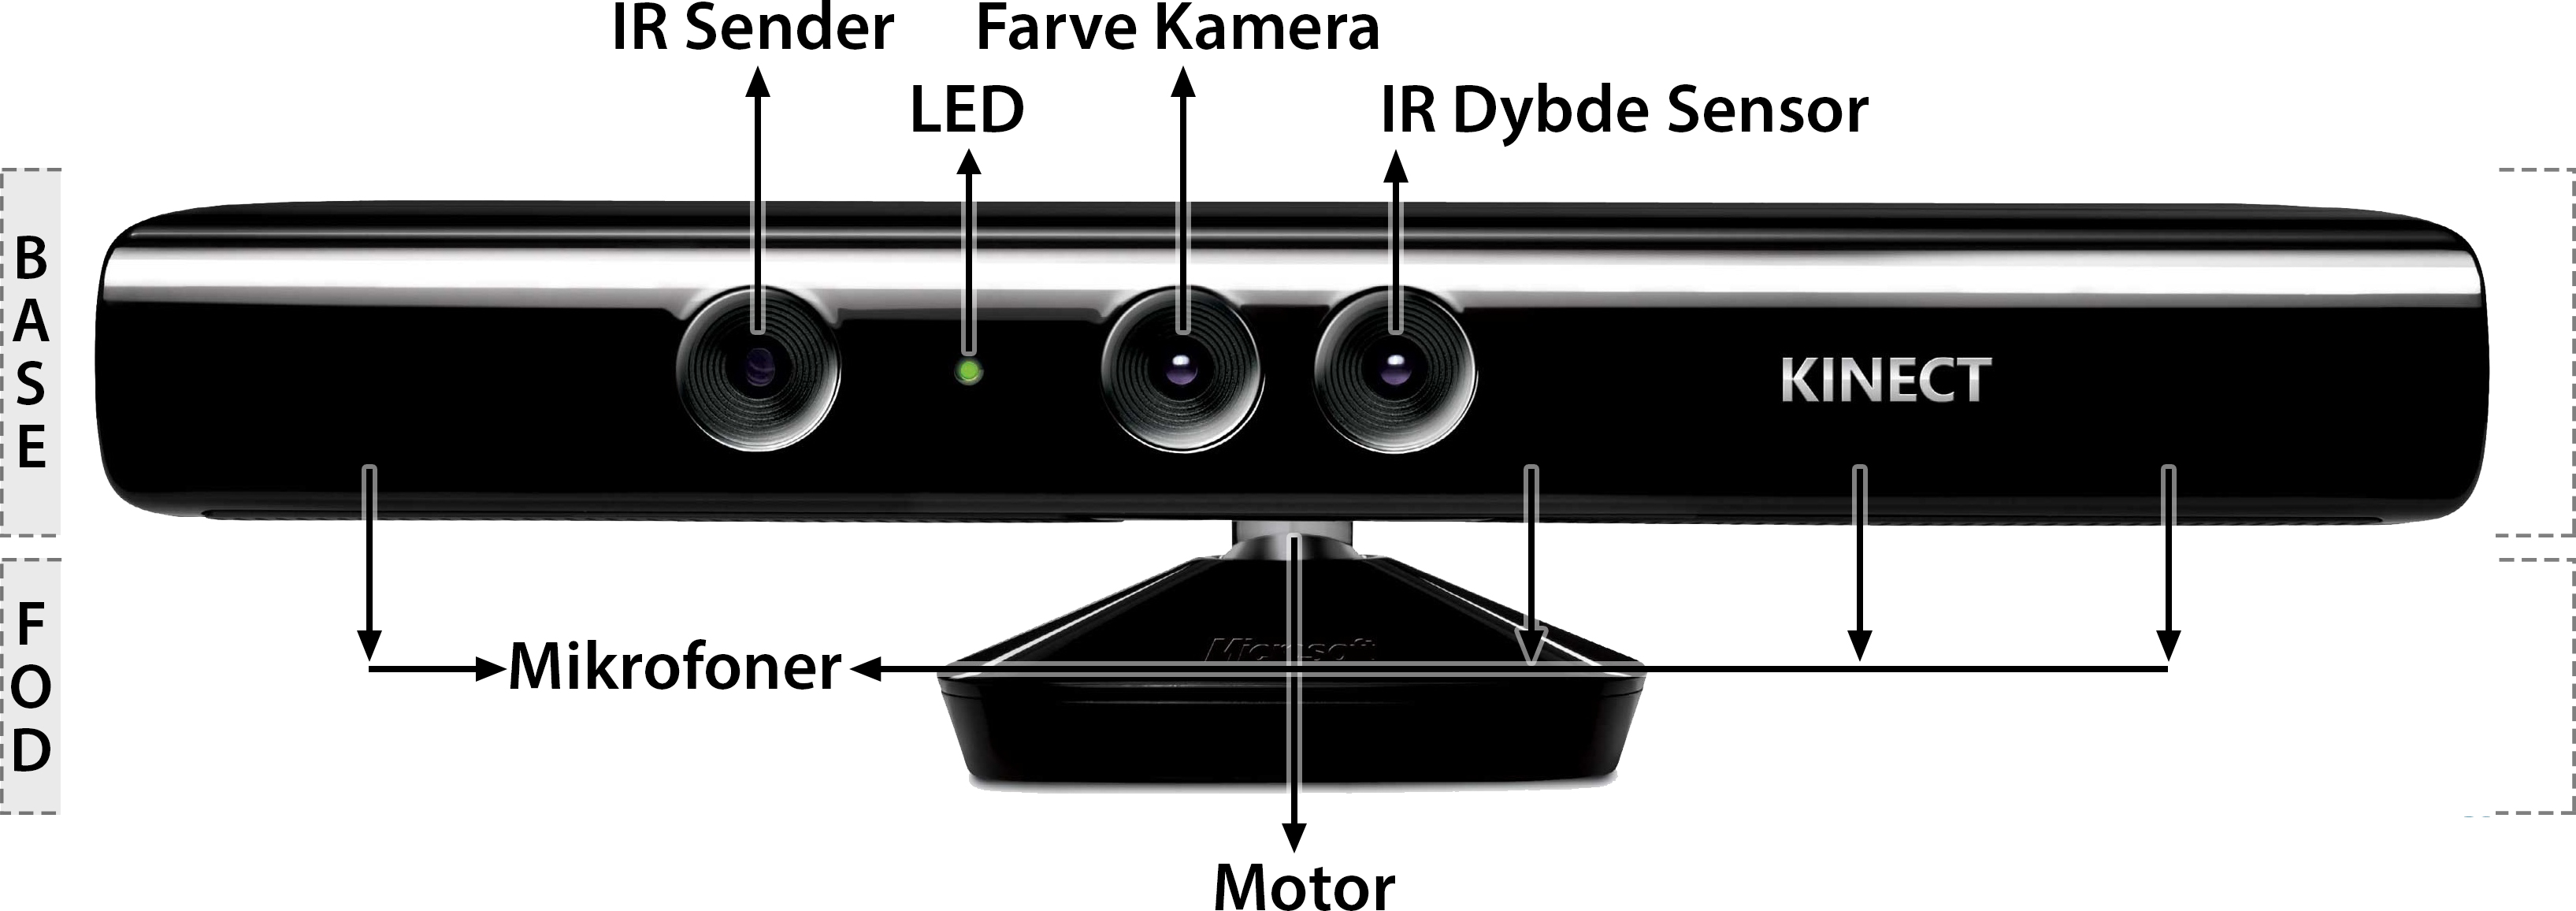
\includegraphics[width=1.0\textwidth]{kinect/kinect}
\caption{Microsoft Kinect for Windows}
\label{kinect:opbygning}
\end{figure}

\subsubsection{Farvekamera}
For at gøre Kinecten i stand til at se, er den udstyret med et farvekamera som er placeret ca. i midten af enheden (jvf. \cref{kinect:opbygning}).
Et farvekamera kan være nyttigt i spil, hvor man ønsker at vise spilleren fysisk på skærmen eller hvis man benytter sin Kinect til gruppechat (som et webcam).
Videoen bliver sendt som en RGB videostrøm med mulighed for en opløsning på 1280x960 med en opdateringshastighed på 12 billeder i sekundet eller en lavere opløsning på 640x480 og 30 billeder i sekundet, hvis man ønsker en mere ”flydende” videostrøm~\cite{kinectForWindowsFeatures}.
Kinecten har en horisontal betragtningsvinkel på 57\degree~og en vertikal betragtningsvinkel på 43\degree, hvilket giver den et vertikalt synsfelt på $\pm 21.5$\degree, hvis den er placeret ift. 0\degree~vandret.
Et visuelt billede af Kinectens betragtningsvinkler kan ses på \cref{kinect:vinkler}.

\begin{figure}
\centering
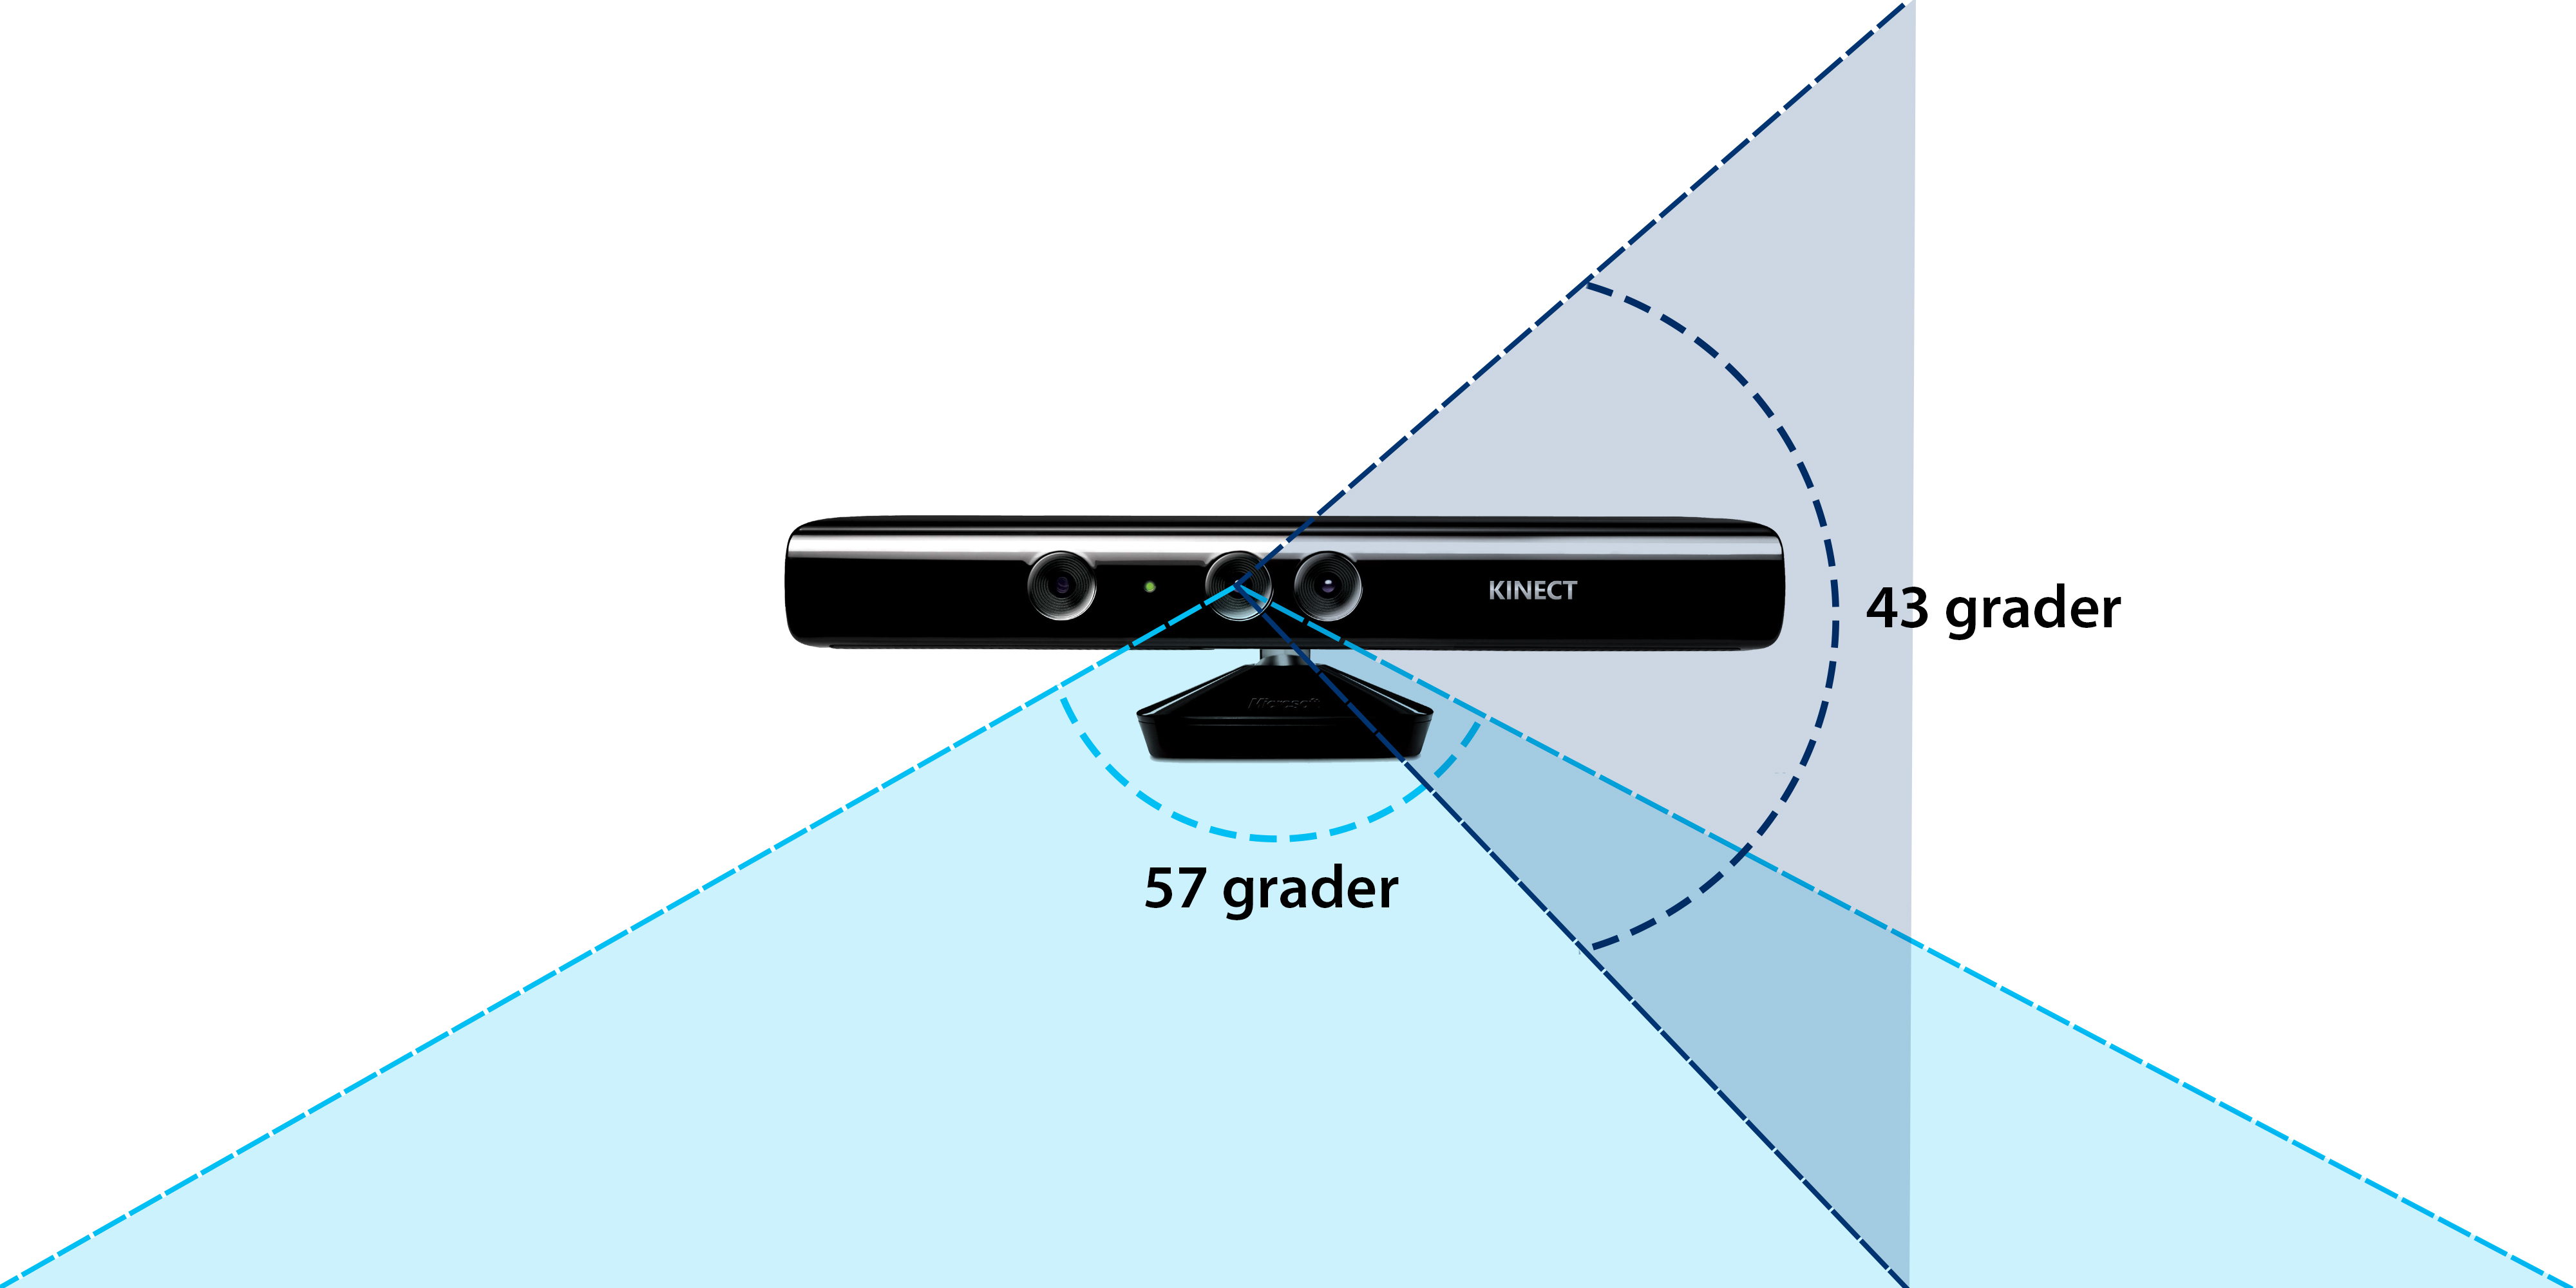
\includegraphics[width=1.0\textwidth]{kinect/kinect_view_angles}
\caption{Betragtningsvinkler for farvekameraet}
\label{kinect:vinkler}
\end{figure}

Disse parametre er interessante i forhold til det hvad Kinecten skal bruges til samt hvilket miljø hvori den skal bruges. Det er f.eks. vigtigt at kende dens betragningsvinkler, hvis den skal benyttes til at lokalisere objekter med, da placeringer af disse skal placeres ift. deres fysiske placering, og ikke kun i Kinectens koordinatsæt.

\subsubsection{Infrarød (IR) sender}
Metoden Kinecten benytter for at bestemme personers placeringer deres afstand fra Kinecten er vha. den infrarøde (IR) sender (\cref{kinect:opbygning}), som udsender et infrarødt lys der reflekteres så snart de rammer et objekt i rummet. 
Disse signaler bliver fanget af en anden sensor på Kinecten; nemlig den infrarøde dybde sensor.

\subsubsection{IR dybde sensor}
Når det infrarøde lys bliver reflekteret tilbage mod Kinecten, bliver det opfanget af dybde sensoren (\cref{kinect:opbygning}), som konverterer lyset til dybde information, hvori man har en per-pixel afstand til de objekter der er tilstede i billedet.

\subsubsection{Mikrofoner}
Kinecten er også i stand til at optage lyd via de indbyggede mikrofoner.
Dette er dog ikke det eneste mikrofonerne kan benyttes til; de kan også benyttes som en alternativ metode til at bestemme afstand og retning fra f.eks. en person der taler.
Rækken af mikrofoner (se \cref{kinect:opbygning}) består af 4 stk. som er placeret på fronten af Kinecten.
En enkelt mikrofon sidder i venstre side mens de tre andre er placeret til højre, hvilket gør det muligt at triangulere lydsignaler for at bestemme retningen af lydkilden.
Flere mikrofoner gør det også muligt at lave ``noise-suppression'' ift. omgivelserne, hvis man benytter Kinect, mens man spiller, til at kommunikerer med sine med-/modspillere således at unødig støj filtreres fra~\cite[s.~15]{kinectProgrammingGuide}.

\subsubsection{Motor til justering af vinklen}
For at gøre det muligt for en Kinect at operere i flere forskellige miljøer og placeringer, er der indbygget en lille motor til at justere vinklen mellem Kinecten og foden den står på (jvf. \cref{kinect:opbygning}).
Den kan bevæge sig fra 0\degree~til 27\degree~ (op) og fra 0\degree~til -27\degree~(ned).
Denne funktionalitet er ideel hvis man ønsker at kalibrere Kinecten ift. dens fysiske placering og de omgivelser man ønsker at bruge den i.
Dog anbefaler Microsoft at man ikke benytter motoren kontinuert i sine programmer, da den ikke tåler vedvarende belastninger~\cite{kinectDocElevationAngle}.

\subsubsection{LED}
Mellem kameraet og IR senderen er der placeret en status LED, der fortæller om driverne til Kinecten er indlæst korrekt eller ej.
Dette kan være nyttigt for udviklere, da det giver sikkerhed for at kommunikationen mellem PC og Kinect er ok~\cite[s.~15]{kinectProgrammingGuide}.

\subsubsection{Accelerometer}
Kinect er også udstyret med et 3-akse accelerometer, som udvider den til andre anvendelsesområder end blot at følge (tracke) objekter og kropsbevægelser.
Det er konfigureret til at give målinger fra -2g til 2g (mere præcis ved langsomme bevægelser end hurtige)~\cite{kinectAccelerometer}.
Målingerne  er opbygget som en 3D vektor som peger mod tyngdekraften (gulv-planet), hvilket f.eks. gør det muligt at detektere om den er monteret korrekt (ovenpå eller under et fladskærms tv), således dens tilt kan korrigeres vha. den indbyggede motor.
En anden interessant anvendelsesmulighed er at accelerometeret kan benyttes til at give bedre 3D projektioner i Augmented Reality.
Ifølge dokumentationen~\cite{kinectDocAccelerometer}, er det præcist ned til en grad, dog med en nøjagtighed der kan varierer med op til 3 grader i forhold til rumtemperaturen.
De skriver endvidere i dokumentationen at der kan kompensateres for denne unøjagtighed ved at sammenligne den vertikale måling (y-aksen i accelerometerets koordinatsystem) med den benyttede gulvplans dybdedata.


\section{Kinect for Windows SDK}
Til Kinecten findes der et officielt SDK\footnote{ Version 1.8, Udgivet 17 september, 2013~\cite{kinectSDK18}}, som åbner op for al funktionalitet i Kinecten med support fra Microsoft.

API'en er bygget op omkring en solid forståelse for menneskers bevægelser og karaktertræk således API'en kan fungere som et interface der kan genkende personers bevægelser, følge ansigter, genkende gestus og tale.
Med Microsoft Kinect Toolkit installeret kan man endvidere få adgang til Kinect Fusion der gør det muligt at rekonstruere 3D objekter ud fra Kinectens kamera og dybdebilleder fra IR sensorerne.~\cite{kinectForWindowsFeatures}


\subsection{Kinect API}\label{kinect:kinectapi}
I dette afsnit vil der blive gennemgået eksempler der demonstrer den basale brug af Kinect API'en.

\subsubsection{Initialisering}
For at initialisere Kinecten og få adgang til dens sensorer skal Kinecten initialiseres.
Et eksempel på initialisering af en Kinect kan se på \cref{kinect:initialisering}. \lstinline[style=csharp]|Form1_Load| metoden i linje \ref{kinect:load} køres ved applikationens opstart og sørger for at starte sensoren hvis den findes. Fra linje \ref{kinect:enablebegin} til \ref{kinect:enableend} tændes for de billedstreams der er nødvendige. I eksemplet tændes for RGB-kameraet, dybdekameraet samt skeletdetektoren. Hvis der ikke er en Kinect tilsluttet meldes der fejl (linje \ref{kinect:error}).

\begin{lstlisting}[style=csharp, label=kinect:initialisering, caption={Initialisering af en Kinect sensor}]
KinectSensor sensor;

private void Window_Loaded(object sender,
	RoutedEventArgs e) (*\label{kinect:load}*)
{
    if (KinectSensor.KinectSensors.Count > 0)
    {
        this.sensor = KinectSensor.KinectSensors[0];
        StartSensors();
        
        this.sensor.ColorStream.Enable();(*\label{kinect:enablebegin}*)    
	this.sensor.DepthStream.Enable();
        this.sensor.SkeletonStream.Enable();(*\label{kinect:enableend}*)
	this.sensor.ColorFrameReady += 
		sensor_ColorFrameReady; (*\label{kinect:event}*)
    }

    else
    {
        MessageBox.Show("No Kinect connected"); (*\label{kinect:error}*)
        this.Close();
    }

}

private void StartSensors()
{
    if (this.sensor != null && !this.sensor.IsRunning)
    {
        this.sensor.Start();
    }
}
\end{lstlisting}

\subsubsection{Visning af Kinectens billeddata}
For at vise de billeder som Kinecten optager benyttes \lstinline[style=csharp]!sensor_ColorFrameReady! eventet. 
Dette event affyres hver gang der modtages et nyt billede fra Kinecten. 
Et eksempel på at vise Kinectens data ses på \cref{kinect:picture}, hvor der i linje \ref{kinect:openframe} gemmes en reference til den frame der netop er blevet optaget af Kinecten.
I linje \ref{kinect:pixeldata} kopieres data over i et bytearray for at arbejde på dataen. 
I linje \ref{kinect:source} sættes billedets source til et billede konstrueret ud fra dataen fra Kinecten.
Billedet \lstinline[style=csharp]|imageFrame| viser nu hvad Kinecten ser.

\begin{lstlisting}[style=csharp,caption={Visning af billeddata fra Kinectens RGB-kamera}, label=kinect:picture]
byte[] pixelData = null;
void sensor_ColorFrameReady(object sender,
	ColorImageFrameReadyEventArgs e)
{
    using (ColorImageFrame imageFrame = 
    	e.OpenColorImageFrame()) (*\label{kinect:openframe}*)
    {
        if (imageFrame == null)
            return;

            this.pixelData = 
            	new byte[imageFrame.PixelDataLength];(*\label{kinect:pixeldata}*)

            imageFrame.CopyPixelDataTo(this.pixelData);

            int stride = imageFrame.Width *
            	imageFrame.BytesPerPixel;

            this.KinectImage.Source = 
            	BitmapSource.Create(
            imageFrame.Width, imageFrame.Height, 
            	96, 96, PixelFormats.Bgr32, null, 
            		pixelData, stride); (*\label{kinect:source}*)
    }
}    
\end{lstlisting}




\section{OpenCV}
% evt. en generel beskrivelse af emgu og openCV
OpenCV (\emph{Open Source Computer Vision Library}) er et Library udviklet af \emph{Intel}
til brug ved Realtids \emph{computer vision}.
OpenCV er skrevet i C++ og er frit tilgængeligt under BSD licensen.

\subsection{beskrivelse af udvalgte klasser og funktioner}

\subsubsection{Metoden findContours}
Metoden findCountours gennemsøger et billede og finder konturer, som den kan returnere 
repræsenteret på forskellige måder, alt efter hvilke parametre metoden kaldes med.

De typiske repræsentationer er CV\_RETR\_EXTERNAL som kun returnere de yderste konturer,
CV\_RETR\_LIST der returnere alle konturer som en liste uden nogen repræsentation af deres hirarki og
CV\_RETR\_TREE som placere konturene i en træstruktur der repræsentere deres hirarki.

Metoden kan benytte sig af flere forskellige metoder til at oversætte konturerne til en kæde af punkter. 
Der er f.eks. CV\_CHAIN\_APROX\_NONE som oversætter konturen til punkter uden nogen form for komprimering.
En anden er CV\_CHAIN\_APROX\_SIMPLE der kun indeholder start og slutpunkter for alle horisontale,
vertikale og diagonale linjestykker, hvilket reducere antallet af punkter og derved algoritmens
pladskompleksitet.
\cite{EmguCVLibDoc}

\subsubsection{Metoden thresholdBinary}
Metoden tresholdBinary tager to parametre som input en threshld værdi og en maksværdi.
Hvis en pixel i billedet har en intensitet højere end threshold værdien, tildeles denne pixel i resultatet til maksværdien.\cite{EmguCVLibDoc}

$$\text{dst}(x,y) = 
\begin{cases} 
max_{val} & \text{if src}(x,y) > threshold \\
0 & \text{if src}(x,y) \leq threshold
\end{cases}
$$

\subsubsection{Metoden AbsDiff}
Metoden tager et andet billede som input og beregner et billede
som er den absolutte differens mellem de to billeder således at.
\cite{EmguCVLibDoc}

$$ \text{dst}(x,y) = \vert \text{imgA}(x,y) - \text{imgB}(x,y) \vert $$

\subsection{Metoden ApproxPoly}
Denne metode generere en aproximation af konturen med færre punkter ved hjælp af Ramer–Douglas–Peucker algoritmen.
\cite{opencvrefman}[s.~269]
Som input tager den en \emph{double} der bruges til at definere resultatets præsition.
\cite{EmguCVLibDoc}

\chapter{Mapping}\label{valg:mapping}
Noget generelt omkring occ-grid!?
\chapter{Opsummering}\label{valg:opsummering}
\thilemann{Den øverste del er mere opsummering, hvor den sidste del er en forklaring af hvad vi gør}
Denne del fokuserer på hvilke metoder og værktøjer der skal til for at løse problemstillingen for projektet.
Den beskriver de individuelle dele og deres formål og dermed også argumentationen for hvorfor netop det pågældende valg er truffet.

Dette afsnit har til formål at belyse sammenhængen af de enkelte dele; altså hvilken funktion de sammenhængende spiller i den tiltænkte implementering:
\\
\\
Da problemet består i at kortlægge en ukendt verden, vil der blive konstrueret en robot, der har til formål at navigerer i den pågældende verden via et indlejret system.
Dette vil blive implementeret på en NXT-enhed.
Systemet, som kører på robotten, skal skrives i programmeringssproget NXC, som er et C-lignende programmeringssprog.

For at robotten effektivt kan løse lokaliseringsproblemet vil den kommunikere med en PC via MindSqualls frameworket.
\thilemann{Bør vi skrive noget om at vi flytter de tunge beregninger til pc?}
PC'en skal være tilkoblet en Microsoft Kinect, og skal via colortracking med Kinectens farvekamera gøre det muligt at søge efter farver på robotten, og derved være i stand til at returnere en position til robotten, når den forespørger det.

Til at bygge kortet, i takt med at robotten navigerer rundt, benyttes et occupancy grid, der gør det muligt at differentiere mellem ledige og optagne celler.
Opdelingen af verdenen i celler, skal gøre det muligt for robotten enten at styrke eller mindske sin tro på, om et område på kortet er fremkommeligt eller ej.

% PART ******************************
\part[Teori]{Teori\\
	\begin{minipage}[c]{10cm}
	\centering
	\vspace{2cm}
	\normalsize{\textnormal{
		\textit{Denne del indeholder den teori der ligger til grund for projektet.
Der beskrives generel notation brugt efterfulgt af mapping teori.
Her beskrives de to sensormodeller og algortimen der opdaterer \textit{occupancy grid}.
Derefter er der teori omkring lokalisering, som indeholder hvordan man konstruerer en vektor mellem to farver i et billede og følger de to farver.
Til sidst er der teori omkring rutplanlægningen, her beskrives den måde robotten sendes rundt i verden på.}
	}}
	\end{minipage}
}
\chapter{Notation og sandsynlighedsteori}
\section{Sandsynlighedsteori}
Som beskrevet i \cref{sensorer} kan robottens viden omkring verdenen den bevæger sig i ikke være komplet pga. måleusikkerheder.\thilemann{Bør vi nævne at den dog kender sin position via kameraet?}
På trods af dette er den nødt til at kunne reagere på den netop tilgængelige viden, hvorfor det er nødvendigt med metoder der gør det muligt at resonerer sig frem til et 'bedste' valg.
Dette afsnit introducerer den nødvendige sandsynlighedsteori for at kunne beskrive hvad der gør sig gældende i en given verden, baseret på robottens observationer af netop denne.

\subsection{Semantik for sandsynlighed}

% Muligvis unødvendig.
\subsubsection{Sandsynlighed som mål over mulige verdener}

Et sandsynlighedsmål $\mu$ er en funktion fra en mængde verdener til mængden af positive reelle tal. 
Hvis det gælder at $\Omega_1 \cap \Omega_2 = {}$, hvor $\Omega_1$ og $\Omega_2$ er mængder af verdener har vi at:
\begin{enumerate}
\item $\mu(\Omega_1 \cup \Omega_2) = \mu(\Omega_1) + \mu(\Omega_2)$
\item Hvis $\Omega$ er mængden af alle verdener vil $\mu(\Omega) = 1$ 
\end{enumerate}

Sandsynlighedsmålet kan udviddes til at dække sandsynligheden for enkelte verdener således at:
$$\mu(\omega) = \mu(\{\omega\})$$

Notationen kan udvides til at dække propositioner hvor $P(\alpha)$ er målet af mængden af verdener, hvor propositionen $\alpha$ er sand.
Det vil sige at:
$$P(\alpha) = \mu(\{\omega \mid \omega \models \alpha \})$$
Her betyder notationen $\omega \models \alpha$ at propositionen $\alpha$ er sand i verdenen $\omega$.

Notationen kan yderligere udvides til at dække \emph{Random Variables}.
\thilemann{stokastiske variabler?}
En sandsynlighedsfordeling $P(X)$ over variablen $ X $, er en funktion fra
domænet for $ X $ til mængden af positive reelle tal.
Således at givet $x \in dom(X)$, vil $P(x)$ være sandsynligheden for at $X = x$.

Denne notation kan også benyttes til at beskrive sandsynligheder af flere variabler.
F.eks. er $P(X,Y)$ en sandsynlighedsfordeling over variablerne $ X $ og $ Y $, således at $P(X = x \wedge Y = y)$, hvor $x \in dom(X)$ og $y \in dom(Y)$ har værdien $P(X = x \wedge Y = y)$.
$X = x \wedge Y = y$ er en proposition og $ P $ er funktionen over propositioner. 

\subsection{Betinget sandsynlighed}

Målet af 'troen' (\textit{belief}) på en given proposition $ h $ baseret på propositionen $ e $, kaldes den betingede sandsynlighed for $ h $ givet $ e $, og skrives $P(h \mid e)$.

Alle en agents observationer om en verden kaldes dens \emph{bevis} og benævnes $ e $.

\anders{Mangler der ikke noget omkring betinget sansynlighed? f.eks. kædereglen og udledning af bayes regel.}

\subsubsection{Bayes Regel}

$$P(h \mid e) = \frac{P(e \mid h) \times P(h)}{P(e)}$$
Hvor $P(h \mid e)$ er den \emph{posterior} sandsynlighed, $P(e \mid h)$ er \emph{likelihood} og $P(h)$ er \emph{prior}. 


\subsection{Binære Bayes filtre med statisk tilstand}\label{bayes_binaerfiltre}
I tilfælde hvor tilstanden er statisk, altså hvor verden ikke ændrer sig over tid, kan der anvendes binære Bayes filtre.
Her kan en \textit{belief} på en given tilstand $x$ beskrives som:
\begin{equation}
bel_t(x) = p(x \mid z_{1:t},u_{1:t}) = p(x \mid z_{1:t})
\end{equation}

Hvor tilstanden $x$ er binær, dvs. enten sand ($x$) eller falsk ($\lnot x$).
Derved har vi at $bel_t(\lnot x) = 1 - bel_t(x)$.
Bemærk desuden at $x$ altid er den samme, og der ikke findes en $x$ for ethvert tidspunkt $t$, da verden er statisk.

\subsubsection{Log Odds}
For at overkomme eventuelle afrundings-unøjagtigheder, indføres der en funktion \textit{log odds ratio}, der konverterer sandsynlighedsværdierne fra $[0;1]$ til $[-\infty;\infty]$.
\anders{Log odds er for at undgå at beyes regel skal kører fast på sansynlighederne 1 eller 0}
Oddset for tilstand $x$ er defineret som forholdet mellem sandsynlighederne for $x$ og $\lnot x$:

\begin{equation}
\frac{p(x)}{p(\lnot x)} = \frac{p(x)}{1 - p(x)}
\end{equation}

Log oddset er logaritmen til forholdet mellem de to sandsynligheder:

\begin{equation}
l(x) := \log \frac{p(x)}{1 - p(x)}
\end{equation}

\subsubsection{Opdaterings algoritme}
\thilemann{Her beskrives celler med anden notation end den angivet i mapping. Bør det ikke være den samme?}
Opdaterings-algoritmen tager \textit{log odds} for en \textit{posterior belief} $l_{t-1}$ for en celle, samt en ny sensor-måling $z_t$, hvor ud fra der returneres en \textit{log odds} for en ny \textit{belief} $l_t$ for cellen.
\thilemann{Der står 'opdaterings-algoritmen' (bestemt ental), men synes ikke det står specielt klart hvad den opdaterer.}
Algoritmen, skrevet i pseudo-kode, kan ses i \cref{alg:binaerbayesfilter}.

\begin{algorithm}[h]
\textbf{BinaryBayesFilter($l_{t-1}, z_t$)} \\
\Indp $l_t = l_{t-1} + \log \frac{p(x \mid z_t)}{1-p(x \mid z_t)} - \log \frac{p(x)}{1-p(x)}$ \\
\Return{$l_t$}
\caption{Binært Bayes filter algoritme}
\label{alg:binaerbayesfilter}
\end{algorithm}


For at få vores \textit{belief} $bel_t(x)$ tilbage ud fra en \textit{log odds} $l_t$, benyttes følgende ligning:
\begin{equation}
bel_t(x) = 1 - \frac{1}{1 + exp\{l_t\}}
\end{equation}

\section{Notation for probabilistisk robotstyring}
Da det er ønskværdigt at kunne give en præcis beskrivelse af robottens positur, dvs. dens position og retning, vil dette afsnit kort introducere den nødvendige notation, som foreslået af Sebsatian Thrun \citep[s. 16-21]{probabilisticRobotics}.

\begin{itemize}
\item \textbf{Tilstand} betegner den tilstand miljøet er i; altså, robottens positur, omkringliggende objekter som vægge, bygninger osv. 
Tilstand kan være \textit{dynamisk} (tilstanden kan ændre sig -- fx position for en person) og \textit{statisk} (tilstanden ændrer sig ikke -- fx position for en bygning).
Tilstand beskrives af variablen $x$, som også indeholder information omkring robotten selv, fx dens \textit{positur}, \textit{hastighed} og dens \textit{sensorer}.

\item \textbf{Tilstand i tiden} $\mathbf{t}$ betegnes af variablen $x_t$ og beskriver den seneste \textit{kendte} tilstand. 
Den forrige seneste måling angives med $x_{t-1}$ og målingen efter den seneste som $x_{t+1}$.

\item \textbf{Målingsdata} indeholder information om robottens omgivelser til et bestemt tidspunkt. 
$z_t$ er således målingsdata til tiden \textit{t}. 
Notationen

$z_{t_1:t_k} = z_{t_1}, z_{t_2}, z_{t_3}, \dots , z_{t_k}$

betegner alle målinger fra tiden \textit{$ t_1 $} til tiden \textit{$ t_k $}
\item \textbf{Kontrol data} indeholder information om ændring af robottens tilstand. 
Kontrol data kan for eksempel være robottens hastighed, eller en aflæsning af en motors odometer, der fortæller hvor mange omdrejninger hjulet har foretaget.
$u_t$ betegner ændringen af robottens tilstand i intervallet fra \textit{t-1} til \textit{t}.
Igen betegner notation

$u_{t_1:t_k} = u_{t_1}, u_{t_2}, u_{t_3}, \dots , u_{t_k}$

mængden af kontrol data fra \textit{$ t_1 $} til \textit{$ t_k $}.
\end{itemize}

\chapter{Mapping}
\stefan{mapping i overskriften, kortlægning i teksten, skal det ensrettes?}
Til at kortlægge rummet robotten befinder sig i, har vi valgt at bruge \textit{occupancy grid}.
Teorien bag denne algoritme vil blive beskrevet i dette afsnit.

\section{Overblik}
Den overordnede tanke bag et occupancy grid er, at lave en ensartet inddeling af sit kort, hvor hver enkelt celle er repræsenteret af en binær \textit{stokastisk variabel}, der fortæller om den pågældende celle er 'optaget' eller ej, hvor optaget betegnes som sandsynligheden $\mathcal{P}(occupied) = 1$.
Til at begynde med initialiseres hver enkelt celle med værdien $\mathcal{P}(occupied) = 0,5$ som en indikation på, at den aktuelle tilstand endnu ikke er kendt.

En 'ledig' celle har således værdien $\mathcal{P}(occupied) = 0$.
En simpel illustration af et occupancy grid map for det kørselsmiljø, der er opstillet for vores robot, kan ses på \cref{map:approx_occupancy_grid}.

\begin{figure}[h] % Kørselsmiljø og et occupancy grid
\centering
	\begin{subfigure}[b]{.45\textwidth}
	\centering
	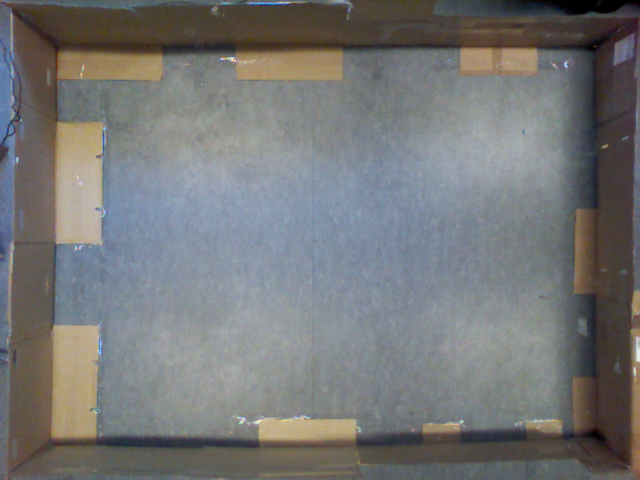
\includegraphics[width=\textwidth]{verden/oppefra}
	\caption{Aktuelt Kørselsmiljø}
	\label{map:world}
	\end{subfigure}
	\begin{subfigure}[b]{.45\textwidth}
	\centering
	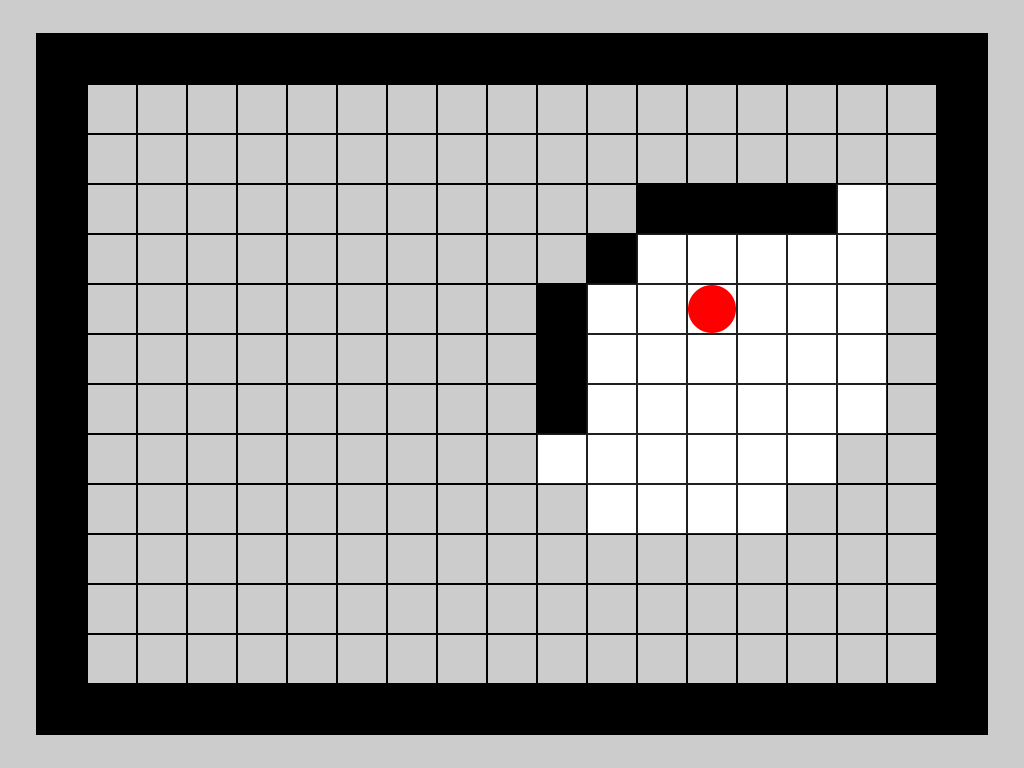
\includegraphics[width=\textwidth]{verden/occupancy_grid_verden}
	\caption{Eksempel på Occupancy Grid}
	\label{map:occupancy_grid}
	\end{subfigure}
\caption{Illustration af et occupancy grid baseret på projekts kørselsmiljø for robotten. Sorte celler i \cref{map:occupancy_grid} indikerer at $\mathcal{P}(occupied) = 1$, hvilket betegner væggene i kørselsmiljøet (\cref{map:world}). Hvide celler indikerer at $\mathcal{P}(occupied) = 0$ og grå celler angiver ikke-udforsket område. Den røde cirkel indikerer robottens position.}
\label{map:approx_occupancy_grid}
\end{figure}

\section{Vertikal og horisontal sensor model}\label{mapping:sensormodel}
Hvis vi antager, at alle objekter i opstillingen er placeret vinkelret til områdets x og y akser,
kan vi konstruere en forholdsvis simpel basal sensormodel.
Først beregner vi afstanden fra robotten til den pågældende celle i vores occupancy grid.

\begin{equation}
r = \mid x_{cell} - x_{robot} + y_{cell} - y_{robot} \mid
\end{equation}

Sensormodellen tildeler de celler, som ligger tæt på den målte afstand fra robotten $z_t$ en højere værdi, kaldet $l_{occ}$, end den prior \textit{belief} $l_0$ fra \cref{eqn:l0}.
De celler som ligger imellem robotten og sensormålingen, tildeles en lavere værdi end $l_0$, kaldet $l_{free}$. 

for at komme frem til hvad tæt på $z_t$ er, indfører vi en konstant $\alpha$ som repræsentere den gennemsnitslige tykkelse af objekter i området.

Sandsynligheden for at cellen er \emph{occupied}, kaldet $l_r$, tildeles således.

\begin{equation}
l_{r} = \begin{cases} 
	l_0 &\text{hvis }r > \text{min}(z_{max},z_t+\frac{\alpha}{2}) \\ 
	l_{occ} &\text{hvis } z_t-\frac{\alpha}{2} \leq r \leq z_t+\frac{\alpha}{2}\\ 
	l_{free} &\text{ellers}  
\end{cases}
\end{equation} \\
Hvor $z_{max}$ er sensorens maksimale måleafstand.
\\
Modellen vil se således ud beskrevet i pseudokode:

\begin{algorithm}[H]
\textbf{inverse_sensor_model($m_i, x_t, z_t$)} \\
Let $x_i,y_i$ be the center-of-mass of $m_i$ \\
$r = |x_i - x + y_i - y|$ \\
\If{$r > min(z_{max}, z_t + \frac{\alpha}{2}$)}{
	\Return{$l_0$}
}
\ElseIf{$z_t - \frac{\alpha}{2} \le r \le z + \frac{\alpha}{2}$}{
	\Return{$l_{occ}$}
}
\Else{
	\Return{$l_{free}$}
}
\caption{Invers sensor model algoritme.}
\label{alg:inversesensormodel}
\end{algorithm}

\subsection{Gaussisk sensor model}\label{mapping:gaussisk}

% forklaring af gaussisk støj (central limit theorem)
% tilfældige fejl vil tilnærme sig en gausssisk kurve.
I modellen, beskrevet i det forgående afsnit, antog vi, at en celle
med afstanden $\frac{\alpha}{2}$ fra robottens måling på $z_t$ havde
samme sandsynlighed som en celle med afstanden 0 fra $z_t$.

Hvis vi antager, at de celler, som ligger tættere på robottens måling, har en større sandsynlighed for at være \emph{occupied}, end dem som ligger tæt på $z_t \pm \frac{\alpha}{2}$, kan vi konstruere en sensor model med en glidende overgang fra værdien $l_{occ}$ for cellen i $z_t$ til værdierne $l_{free}$ og $l_0$ for cellerne på position $z_t \pm \frac{\alpha}{2}$. 

Da summen af uafhængige fejlmålinger, ifølge \emph{central limit theorem} vil tilnærme sig
den gaussiske normalfordeling, vil det være en god approximation for robottens måleusikkerhed.\cite[p. 223]{ArtificialIntelligence}

For at finde en passende normalfordeling skal vi vælge en passende middelværdi og en passende standard afvigelse. 
Vi ved at centrum, dvs. middelværdien, for fordelingen skal være målingen $z_t$.

\begin{figure}
\centering 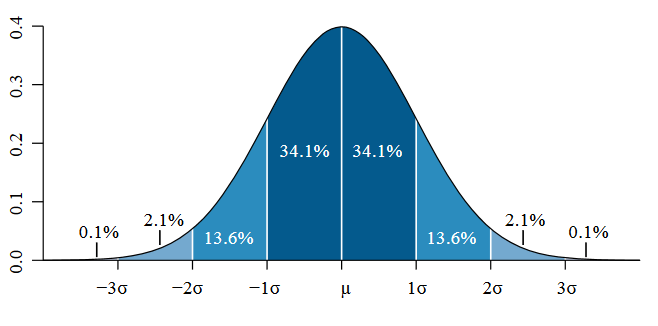
\includegraphics[scale=.75]{NormalDist}
\caption{Normal fordeling $\mathcal{N}(\mu,\sigma^2)$.}
\label{normaldistimg}
\end{figure}

Udfra \cref{normaldistimg} kan vi se, at det vil være passende hvis $\frac{\alpha}{2}$ svarer til tre standard afvigelser. dvs.
\begin{equation}
	3\sigma = \frac{\alpha}{2} \implies \sigma = \frac{\alpha}{6}
\end{equation}

Vi kan anvende den passende normalfordeling $\mathcal{N}(z_t,\big(\frac{\alpha}{6}\big)^2)$ der ses her. 

\begin{equation}
\mathcal{N}\bigg(z_t,\bigg(\frac{\alpha}{6}\bigg)^2\bigg) = 
\frac{1}{\sqrt{2 \pi \big(\frac{\alpha}{6}\big)^2}}e^{- \frac{(x - z_t)^2}{2 (\frac{\alpha}{6})^2}}
\end{equation}

Vi kan beregne en sandsynlighed, for en celle i afstand $r$, udfra normalfordelingen ved at tage integralet af fordelingen på følgende måde.

\begin{equation}
P(r) = \lim \limits_{\rho \to 0} \bigint_{r-\rho}^{r+\rho} \frac{1}{\sqrt{2 \pi \big(\frac{\alpha}{6}\big)^2}}e^{- \frac{(x - z_t)^2}{2 (\frac{\alpha}{6})^2}}\, \mathrm{d}x
\end{equation}

% Indsæt billede som viser hvorden mapningen vil se ud.

Da vi vil have at sandsynlighederne mellem $z_t-\frac{\alpha}{2}$ og $z_t$ går i en glidende overgang fra $P_{free}$ til $P_{occ}$,
mens vi vil have en overgang fra $P_{occ}$ til ${P_0}$ for afstande imellem $z_t$ og $z_t+\frac{\alpha}{2}$.
Har vi valgt at lave en linær mapning, af de sandsynligheder vi får fra normalfordelingen til de to intervaller, ved hjælp af linjens ligning.
Her er $P_{occ}$,$P_{free}$ og $P_0$ sandsynlighederne for henholdsvis $l_{occ}$,$l_{free}$ og $l_0$.


\begin{equation}
	P_\kappa(r) = \begin{cases}
		\frac{P_{occ}-P_0}{P(z_t)-P(z_t+\frac{\alpha}{2})}(r-P(z_t))+P_{occ} &\text{hvis } z_t < r \\
		\frac{P_{free}-P_{occ}}{P(z_t-\frac{\alpha}{2})-P(z_t)}(r-P(z_t))+P_{occ} &\text{hvis } z_t \geq r 
	\end{cases}
\end{equation}

%######################################

%Da vi vil have, at sandsynligheden i centrum af fordelingen er den samme, som sandsynligheden fra $l_{occ}$ ganger vi med konstanten $\eta$, for på den måde at strække fordelingen så den passer. 

%\begin{equation}
%	P_\eta(r) = \eta P(r) 
%\end{equation}

%For at beregne $\eta$ udfra $l_{occ}$ benytter vi os af \cref{logodds:bel}.

%\begin{equation}
%	\eta P(r) = 1 - \frac{1}{1+e^{l_{occ}}} \implies \eta = \frac{1-\frac{1}{1+e^{l_{occ}}}}{P(r)}
%\end{equation}

%########################################

%\begin{equation}
%	\begin{split}
%		&\eta \lim \limits_{\rho \to 0} \bigint_{z_t-\rho}^{z_t+\rho} \frac{1}{\sqrt{2 \pi \big(\frac{\alpha}{6}\big)^2}}e^{- \frac{(x - z_t)^2}{2 (\frac{\alpha}{6})^2}}\, \mathrm{d}x = 1 - \frac{1}{1+e^{l_{occ}}} \\ 
%	&\implies \eta = \frac{1 - \frac{1}{1+e^{l_{occ}}}}{\lim \limits_{\rho \to 0} \bigint_{z_t-\rho}^{z_t+\rho} \frac{1}{\sqrt{2 \pi \big(\frac{\alpha}{6}\big)^2}}e^{- \frac{(x - z_t)^2}{2 (\frac{\alpha}{6})^2}}\, \mathrm{d}x}
%	\end{split}
%\end{equation}

Den nye tildeling af sandsynlighed til cellen vil nu se således ud.

%\begin{equation}
%	l_{r} = \begin{cases} 
%		l_0 &\text{hvis }r > \text{min}(z_{max},z_t+\frac{\alpha}{2}) \\
%		max\Bigg(l_{0},log\Big(\frac{P_\eta(r)}{1-P_\eta(r)}\Big)\Bigg) &\text{hvis } z_t < r \leq z_t+\frac{\alpha}{2} \\
%		max\Bigg(l_{free},log\Big(\frac{P_\eta(r)}{1-P_\eta(r)}\Big)\Bigg) &\text{hvis } z_t-\frac{\alpha}{2} \leq r \leq z_t \\
%		l_{free} &\text{ellers}	
%	\end{cases} 
%\end{equation}
%Hvor $l_0$ er defineret i \cref{eqn:l0} og $z_{max}$ er sensorens maksimale måleafstand.

\begin{equation}
	l_{r} = \begin{cases} 
		l_0 &\text{hvis }r > \text{min}(z_{max},z_t+\frac{\alpha}{2}) \\
		log\Big(\frac{P_\kappa(r)}{1-P_\kappa(r)}\Big) &\text{hvis } z_t < r \leq z_t+\frac{\alpha}{2} \\
		log\Big(\frac{P_\kappa(r)}{1-P_\kappa(r)}\Big) &\text{hvis } z_t-\frac{\alpha}{2} \leq r \leq z_t \\
		l_{free} &\text{ellers}	
	\end{cases} 
\end{equation}
Hvor $l_0$ er defineret i \cref{eqn:l0} og $z_{max}$ er sensorens maksimale måleafstand.



%
%\subsection{Generel udgave af sensor modellen}
%
%% objekter kan placeres i alle vinkler
%
%\subsubsection{Generel model med gaussisk støj}
%
%% gaussisk støj i 2-d
%
%
%\subsection{tilpasset sensor model}
%
%
%% overfitting
%
%\subsection{sensor model baseret på målinger}
%
%% fejl i sensor er ikke nødvendigvis 'tilfældige' eller uafhængige
%% en generel sensormodel som benytter en sandsynlighedsdistribution som vi selv har målt.
%
%
%\subsection{data udledet udfra robottens placering}
%
%% forbedring hvor vi tager højde for robotten
%
%
%\section{Forward Sensor Model	}
%
%
%














\

% !TeX spellcheck = da_DK
\section{Occupancy Grid algoritmen}
Dette afsnit vil gennemgå algoritmen, der skal opdatere et occupancy grid.
Algoritmen er taget fra \cite[p. 286]{probabilisticRobotics}.
Formålet med \textit{occupancy grid} algoritmen er, at beregne	et nyt kort ud fra et kort og en samling data:

\begin{equation}
p(m \mid z_{1:t}, x_{1:t})
\end{equation}

hvor $m$ er et kort, $ z_{1:t} $ er mængden af målinger op til tiden $t$ og $ x_{1:t} $ er robottons rute i form af en følge af \textit{poses}.

Kortet er inddelt i et finit antal celler.
Hver celle kan findes ved $ m_i $ hvor $i$ er cellens indeks. 
Hele kortet kan derfor betegnes

\begin{equation}
m = \sum_{i}^{} m_i 
\end{equation}

Hver celle er tilknyttet en binær værdi der betegner hvorvidt cellen er \textit{occupied} eller \textit{free}.
Værdien 1 betegner \textit{occupied}, mens 0 betegner \textit{free}.

For at begrænse mængden af celler, der skal beregnes ved en opdatering af et occupancy grid, nedbrydes problemet til en mængde delproblemer af formen

\begin{equation}
p(m_i \mid z_{1:t}, x_{1:t})
\end{equation} 

Da der nu er et problem af denne type for hver celle, kan man nøjes med kun at opdatere de celler, der er ny information om.

Som i det originale binære filter (se evt. \cref{bayes_binaerfiltre}) benyttes log odds repræsentationen til at udtrykke om en celle er optaget

\begin{equation}
l_{t,i} = log{ \frac{p(m_i \mid z_{1:t}, x_{1:t})}{1 - p(m_i \mid z_{1:t}, x_{1:t})}} 
\end{equation} 

Sandsynligheden findes ud fra log odds repræsentationen ved

\begin{equation}
p(m_i \mid z_{1:t}, x_{1:t}) = 1 - \frac{1}{1 + exp \{ l_{t,i} \} }
\end{equation} 

\Cref{occupancygrid:alg} viser hvordan værdierne i et occupancy grid kunne opdaterer de celler, der er relevante for en aktuel sensormåling. 
Til opdateringen bruges \textbf{inverse\_sensor\_model} som findes i \cref{mapping:sensormodel}.\thilemann{Dobbelttjek lige at denne henvisning er korrekt}
Værdien $ l_0 $ er den a priori værdi for, om cellen er optaget repræsenteret som log odds

\begin{equation}
  l_0 =  log \frac{p(m_i = 1)}{p(m_i = 0)} = log \frac{p(m_i)}{1- p(m_i)}
\end{equation} 

\begin{algorithm}[H]
\LinesNumbered
OccupancyGridMapping( \{$ l_{t-1,i} $ \}, $ x_t $, $ z_t $):

\ForAll{cells $ m_i $}
{
\eIf{$ m_i $ is in perceptual field of $ z_t $ \\}
%then
{ $ l_{t,i} = l_{t-1,i} $ + \textbf{inverse\_sensor\_model} $( m_i, x_t, z_t ) - l_0$\\ }
%else
{ $ l_{t,i} = l_{t-1,i}  $\\ }
}
\Return {$ \{l_{t,i}\} $}
\caption{Occupancy grid opdateringsalgoritmen.}\label{occupancygrid:alg}
\end{algorithm}





\chapter{Lokalisering}
Til lokalisering af robotten anvendes en \kinect (se evt. \cref{kinect:argumentation}).
Denne er udstyret med et farvekamera (se evt. \cref{kinect:farvekamera}), der vil blive anvendt til at bestemme robottens placering.
Ved at udstyre robotten med to mærkninger i klare farver, vil det på billeder fra Kinecten være muligt at lokalisere robotten.

I det følgende beskrives den anvendte metode til lokalisering af robotten.
Først beskrives den overordnede metode, hvorefter forbedringer af metoden præsenteres.

\section{Farveforskel}\label{tracking:colordiff}
%Beskrivelse af den metode der anvendes til at beskrive forskellen mellem farver
Lokalisering af robotten foretages som udgangspunkt ud fra \'et billede.
Det vil sige, at systemet skal være i stand til at lokalisere robotten ud fra \'et billede alene.
Som beskrevet ovenfor udstyres robotten med to mærkninger i klare farver, som skal spores.
Det er altså målet at finde de dele af et enkelt billede, der matcher bestemte farver.

\subsection{Match af farver}
For at vurdere om to farver matcher hinanden, må det først gøres klart, at det ikke kan forventes at matche en farve eksakt.
Til dette spiller faktorer som lys og skygge for stor en rolle.
I stedet tages der udgangspunkt i en søgt farve, og ud fra denne ledes der efter alle \textit{nære} farver.
Til dette formål betragtes den farve-repræsentation der arbejdes med.
Farver repræsenteres ved tre værdier; rød, grøn og blå (også kaldet RGB), der angiver alle de mulige farver for en pixel i et billede.
Ved at betragte de tre farver som hver sin dimension i et tredimensionelt rum, kan farver repræsenteres som vektorer.
Hermed bliver det muligt at tale om forskellen på to farver som \textit{afstanden mellem to farver}.

\begin{figure}
\centering
\tdplotsetmaincoords{60}{110}
\begin{tikzpicture}[scale=5,tdplot_main_coords]

%set up some coordinates 
%-----------------------
\coordinate (O) at (0,0,0);
\tdplotsetcoord{P1}{1.1}{60}{30}
\tdplotsetcoord{P2}{1.5}{40}{60}

%draw figure contents
%--------------------

%draw the main coordinate system axes
\draw[ultra thick,red,->] (0,0,0) -- (1,0,0) node[anchor=north east]{$r$};
\draw[ultra thick,green,->] (0,0,0) -- (0,1,0) node[anchor=north west]{$g$};
\draw[ultra thick,blue,->] (0,0,0) -- (0,0,1) node[anchor=south]{$b$};

\draw[-stealth,color=gray] (O) -- (P1);
\draw[-stealth,color=gray] (O) -- (P2);
\draw[-stealth,thick] (P1) -- (P2);

\draw (P1) node[anchor=west]{$C_1$};
\draw (P2) node[anchor=west]{$C_2$};

%draw projection on xy plane, and a connecting line
\draw[dashed, color=gray] (O) -- (P1xy);
\draw[dashed, color=gray] (P1) -- (P1xy);

\draw[dashed, color=gray] (O) -- (P2xy);
\draw[dashed, color=gray] (P2) -- (P2xy);

%\draw[dashed] (P1xy) -- (P2xy);
%\draw[dashed] (P2) -- (P2xy);


\end{tikzpicture}
\caption{To farver repræsenteret i et tredimensionelt rum.}
\label{tracking:colorspace}
\end{figure}

På \cref{tracking:colorspace} ses et eksempel på afstanden mellem to farver.
Her er farverne $C_1$ og $C_2$ illustreret med vektorer.
Forskellen på de to farver udtrykkes ved længden af differencen mellem de to.
Altså har vi, for to farver $C_a$ og $C_b$, følgende afstand:
\begin{equation}
dist_{C_aC_b} = |C_a - C_b|
\end{equation}
Hver af de tre RGB farver repræsenteres ved 1 byte og afstanden mellem to farver kan derfor højst være $\sqrt{3 \cdot 255^2} \approx 442$ (forskellen på hvid og sort).

\subsection{Maksimal afstand}\label{tracking:maksimal_afstand}
Det er dog kun interessant at kigge på de farver der ligger i en vis afstand af hinanden.
Der indføres derfor en konstant $\rho$, der definerer et maksimum for hvor langt to farver må være fra hinanden, før de ikke længere er interessante.
I \cref{tracking:adjust} beskrives bestemmelsen af denne konstant.
Med $\rho$ i mente kan der udregnes en vægt, der bestemmer hvor interessant en farve er i forhold til en anden farve.
Lad $C_a$ og $C_b$ være to farver, da har vi:
\begin{equation}
w_{C_aC_b} = \left\{ 
  \begin{array}{r l}
        0 & \quad \text{hvis $dist_{C_aC_b} > \rho$} \\
       1 - \frac{dist_{C_aC_b}}{\rho} & \quad \text{hvis $dist_{C_aC_b} \leq \rho$}
  \end{array} \right.
\end{equation}
Her udtrykker $w_{C_aC_b}$ vægten af interesse for $C_b$ i forhold til $C_a$.
Det følger desuden af ovenstående, at $w_{C_aC_b} \in [0;1]$ for ethvert par af farver.

Ved at undersøge alle pixels i et billede fra kinecten ud fra en bestemt farve, kan vægten af alle pixels bestemmes.
Vægten af en pixel beskriver hvor interessant den er.
Således er pixels med vægt 0 ikke interessante.
De resterende pixels betegnes herefter som \emph{interessante pixels}.

\mikkel{Indsæt evt. sort/hvid billede af tracking}

Ved at finde den mindste firkant der spænder over alle interessante pixels og udvælge dens centrum kan farvens (og dermed robottens) \textit{position} nu bestemmes.

\section{Forbedringer}\label{tracking:improvements}
For at teste implementeringen af ovenstående, blev det forsøgt at lokalisere forskellige farver for varierende $\rho$-værdier.
Af dette fremgik det tydeligt, at metoden var effektiv til genkendelse af farver.
Der blev dog ved testen introduceret tre problemstillinger:
\begin{enumerate}
\item Dele af billedet indeholdt \emph{farve-støj}.
Ved farvestøj forstås pixels der ligger i tæt farve-afstand til den søgte farve, men langt fra det eftersøgte objekt.
\item Farveændringer som følge af lys/skygge.
I takt med at robotten bevæger sig vil lys falde forskelligt på de farvede overflader.
Dette betyder at farven opfanget af kameraet ikke længere matcher den søgte farve godt.
Ofte kan robotten ikke spores hvis belysningen ændres for meget.
\item Funktionens opdateringshastighed var ikke tilfredsstillende (0-3 billeder i sekundet).
Omend intet krav var stillet til opdateringshastigheden, er det dog nødvendigt til enhver tid at kunne beskrive robottens lokation.
Ved lave opdateringshastigheder bliver ændringerne i robottens lokation for høje (robotten flytter sig op til 30 cm mellem to billeder).
\end{enumerate}

I det følgende beskrives de metoder, der er anvendt til at løse ovenstående problemstillinger.
I \cref{tracking:adjust} beskrives resultatet af indførelsen af disse metoder.

\subsection{Filtrering af støj}
\bruno{Nicolaj spørger: Kan det illustreres med et par eksempler?}
%Beskrivelse af implementationen af mean-filter
Den beskrevne \emph{farve-støj}, der opstår i visse billeder, fjernes ved at anvende en variation af et 3x3 median-filter\cite{medianfilter}.
I filteret betragtes alle værdier som binære (0 eller ikke 0).
Midten af boksen erstattes af 0 hvis kun få naboer ikke har værdien 0.
Variablen $\sigma$ indføres her til at beskrive 'få naboer'.
Lad $w_{x,y}$ beskrive vægten af den pixel i et billede, der har koordinat-sæt $x,y$ og $N_{x,y}$ beskrive de \emph{højst} 8 nabo-vægte til dette koordinat-sæt, da kan filteret beskrives således:
\begin{equation}\label{tracking:eq:filter}
w_{x,y}' = \left\{ 
  \begin{array}{r l}
        0 & \quad \text{hvis $|V_{x,y}| < \sigma$} \\
        w_{x,y} & \quad \text{hvis $|V_{x,y}| \geq \sigma$}
  \end{array} \right.
\end{equation}
$$\text{hvor } V_{x,y} = \{ w \in N_{x,y} \mid w > 0 \}$$
Ved at anvende ovenstående filter på alle koordinat-sæt fjernes noget af den uønskede farve-støj.
Filteret påføres gentagne gange, indtil ingen vægte opdateres.
Herefter anses støjen som fjernet.

\subsection{Farve-afstand}
%Beskrivelse af farve-afstand optimering, ved opdatering af den søgte farve
Som løsning på problemet med lys og skygge foretages en løbende opdatering af den farve der søges efter.
Dette gøres ved, for hver opdatering, at finde den højeste vægt (efter filtrering) og dermed den farve, der er tættest på den søgte farve.
Denne farve anvendes efterfølgende som den søgte farve.
På denne måde opdateres den søgte farve løbende og tilpasser sig dermed de forskellige lys/skygge forhold.

\subsection{Afgrænset område}
%Beskrivelse af opdatering af det område der afsøges
En simpel løsning på at optimere den tid det tager at afsøge billedet, er ved at reducere problemets størrelse, altså mængden af pixels, der søges i.
Som et led i lokaliseringen bestemmes den mindste firkant, der spændes over alle interessante pixels.
Ved næste opdatering tages der udgangspunkt i, at robotten ikke har bevæget sig meget.
Problemet kan derfor reduceres til kun at løse samme problem, men for et mindre billede.
Omend robotten ikke bevæger sig meget, er det naturligvis nødvendigt at opfange den lille ændring, der måtte være.
Derfor skal ovennævnte firkant udvides til at spænde over robottens opdaterede position.

På denne måde reduceres problemet, og det kan derfor løses hurtigere.
Bemærk at der i denne løsningsmetode tages udgangspunkt i, at robotten bevæger sig korte afstande mellem opdateringer.
Da den ønskede effekt, ved at indføre denne metode, er hurtigere opdateringer af robottens lokation, vil afstanden robotten kan bevæge sig mellem opdateringer også reduceres.
Der indføres her endnu en variabel $\omega$, der skal beskrive i hvilken grad problemet kan reduceres.
Reduceres problemet ikke tilstrækkeligt, vil robotten stadig bevæge sig for store afstande i mellem opdateringer.
Reduceres problemet derimod for meget, vil det reducerede problem ikke være af tilstrækkelig størrelse til at opfange ændringerne i robottens position.
Herunder følger en beskrivelse af indførelsen af $\omega$:

Lad $R^n$ være den firkant der spænder over alle interessante vægte i løsningen af et problem(beskrevet i \cref{tracking:maksimal_afstand}).
Denne defineres ved to diagonalt modsatte punkter:
{
\newcommand{\cvec}[2]{\begin{pmatrix}#1\\#2\end{pmatrix}}

$$R^n = \left\{\cvec{x_1}{y_1}, \cvec{x_2}{y_2}\right\} \mid x_1 \leq x_2 , y_1 \leq y_2$$
Ud fra denne definition kan det reducerede problems størrelse $R^{n'}$ nu defineres:
\begin{equation}\label{tracking:eq:inflate}
R^{n'} = \left\{
	\cvec{R^n_{x_1}-\omega}{R^n_{y_1}-\omega},
	\cvec{R^n_{x_2}+\omega}{R^n_{y_2}+\omega}
\right\}
\end{equation}
Herved er det reducerede problems størrelse, beskrevet med udgangspunkt i det forrige problems løsning som illustreret på \cref{tracking:reduction}.
}

\begin{figure}
\centering
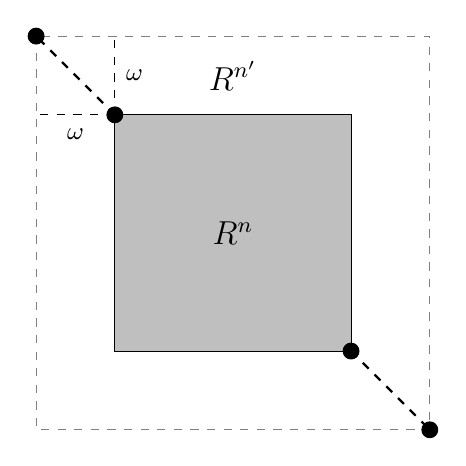
\begin{tikzpicture}[scale=.5]

%set up some coordinates 
%-----------------------
\coordinate (C1) at (0,10); % Outer top left
\coordinate (C2) at (10,0); % Outer bottom right
\coordinate (C3) at (2,8); % Inner top left
\coordinate (C4) at (8,2); % Inner bottom right

%draw figure contents
%--------------------

\draw [fill=lightgray] (C3) rectangle (C4); % Inner rectangle
\draw[dashed, color=gray] (C1) rectangle (C2); % Outer rectangle

\draw [fill] (C1) circle [radius=0.2]; % Outer top left
\draw [fill] (C2) circle [radius=0.2]; % Outer bottom right
\draw [fill] (C3) circle [radius=0.2]; % Inner top left
\draw [fill] (C4) circle [radius=0.2]; % Inner bottom right

\draw[thick,dashed] (C3) -- (C1); % Inner top left to outer top left
\draw[thick,dashed] (C4) -- (C2); % Inner bottom right to outer bottom right

\draw[dashed] (C3) -- (0,8);
\draw[dashed] (C3) -- (2,10);

\draw (5,5) node {\large $R^n$};
\draw (5,9) node {\large $R^{n'}$};

\draw (1,7.5) node {\small $\omega$}; % x1-w
\draw (2.5,9) node {\small $\omega$}; % y1-w

\end{tikzpicture}
\caption{Søgning efter robotten begrænset til $R^n$'s $\omega$ nærmeste pixels.}
\label{tracking:reduction}
\end{figure}

\section{Justering}\label{tracking:adjust}
%Beskrivelse af diverse thresholds og hvilke værdier "der fungerer"
Af de forrige afsnit fås tre variable, der søges justeret således, at de løser de beskrevne problemer tilfredsstillende.
Herunder listes de tre variable, samt en beskrivelse af deres betydning og endelig justering.

Bemærk at værdierne der tildeles variablerne \emph{ikke} er uafhængige.
Ændringer i $\omega$ har således betydning for opdateringshastigheden, hvilken igen har betydning for $\rho$.
Ligeledes har $\rho$ betydning for hvor hvilke pixels der er interessante samt i hvor høj grad der findes støj i de udregnede vægte, hvilket har betydning for $\sigma$ etc.

Værdierne er derfor justeret i takt med, at de forskellige løsninger er implementeret, hvorfor de endelige værdier kan ses herunder.

\begin{description}
\item[Farve afstand (${\boldsymbol{\rho}}$)]
Som nævnt i \cref{tracking:colordiff} er den maksimale afstand mellem to farver 442 (forskellen på sort og hvid).
Den minimale afstand mellem to farver er 0, hvilket er tilfældet for to ens farver.
Altså skal $\rho$ bestemmes mellem disse to.
For den maksimale afstand betragtes alle pixels som interessante, mens det for den minimale kun vil være pixels med den eksakte farve, der søges efter.
Da interessante pixels skal have en farve, der er \emph{tæt på} den søgte, vil $\rho$ have en værdi tættere på 0.
Det er ved forsøg bestemt at:
$$\rho = 50$$
Hvilket angiver, at farver med afstand større end 50 \emph{ikke} er interessante at betragte i løsningen.
%441,672955930063709849498817084

\item[Filter \textit{naboer} ($\boldsymbol{\sigma}$)]
I \cref{tracking:improvements} blev det beskrevet at $\sigma$ højst kan være 8, da en pixel har 8 \emph{naboer}.
Vælges $\sigma = 8$ fremgår det af \cref{tracking:eq:filter} at et sådant filter vil fjerne alt information i billedet.
Vælges derimod $\sigma = 0$ (som er minimum værdi for $\sigma$) vil filteret ingen effekt have.
Det er ved forsøg bestemt at:
$$\sigma = 4$$
Som fjerner alle vægte med færre end 4 interessante nabo-pixels.

\item[Problem reduktion ($\boldsymbol{\omega}$)]
Den kraftigste reduktion af problemets størrelse, uden reduktion af $R^n$, vil være $\omega = 0$ (se \cref{tracking:eq:inflate}) der angiver, at der kun skal søges i den forrige løsnings område, og altså at robotten ikke har flyttet sig.
Dette betyder reelt, at det må gælde at $\omega > 0$.
Der er imidlertid ingen øvre grænse for $\omega$, omend det følger naturligt at jo kraftigere en reduktion der foretages, des hurtigere kan en opdatering ske.
Det er ved forsøg bestemt at:
$$\omega = 5$$
Altså vil firkanten, der indkapslede det forrige resultat udvides med 5 pixels i alle fire retninger (\cref{tracking:reduction}).
Igennem forsøg fremgik det tydeligt at reduktionen i størrelse har en kraftig effekt på opdateringshastigheden.
Derved kunne $\omega$ sættes lavt og en hurtig opdateringshastighed kunne opnås.
I \cref{tracking:updatespeed} beskrives i hvilken grad farvesøgningen forbedredes som følge af $\omega = 5$.
\end{description}

\section{Opdateringshastighed}\label{tracking:updatespeed}
Farvebilleder fra Kinecten kan indsamles på to forskellige måder:
\begin{itemize}
\item I opløsningen 640x480 ved 30 billeder i sekundet
\item I opløsningen 1280x960 ved 15 billeder i sekundet
\end{itemize}

I tabellen herunder præsenteres den opdateringshastighed, der blev opnået i farvesøgning, både med og uden reduktion af problemets størrelse.
Målingerne herunder er kun \emph{omtrentlige}.

{
\newcommand{\mr}[1]{\multirow{2}{*}{#1}}
\newcommand{\ce}[1]{\multicolumn{1}{c|}{#1}}

\begin{table}[h]
\centering
\begin{tabular}{| l | r | r |}
\hline
& \ce{Opdateringer} & \ce{Bevægelse}\\
& \ce{pr. sekund} & \ce{pr. opdatering}\\\hline
640x480&\mr{$2-3$}&\mr{$5-10$cm}\\
Ingen reduktion&&\\\hline
640x480&\mr{$29-30$}&\mr{$<1$cm}\\
Med reduktion&&\\\hline
1280x960&\mr{$<1$}&\mr{$20-30$cm}\\
Ingen reduktion&&\\\hline
1280x960&\mr{$12-13$}&\mr{$<1$cm}\\
Med reduktion&&\\\hline
\end{tabular}
\caption{Opdateringshastighed af farvesøgning med og uden reduktion af problemets størrelse.}
\end{table}}
%
%%Bemærk at implementationen af farve-afstand og afgrænset område forudsætter 'høj' fps
%
%Distance threshold: \rho
%Neighbour threshold: \sigma
%Inflation 'threshold': \omega
%
%640x480 - NoBounds
%3-4fps, 5-10cm
%
%1280x960 - NoBounds
%<1fps, 20-30cm
%
%640x480 - Bounded
%29-30fps, <1cm
%
%1280x960 - Bounded
%12fps, <1cm
%
\section{Omregning fra punkt i billede til reelt punkt}\label{lokalisering:punktomregning}
Det billede der fås ind fra kameraet, består af en mængde pixels.
Robottens centrum, og derved lokation, vil være i præcist én pixel.
For at robotten skal kunne bruge denne til at navigere i den virkelige verden, er det nødvendigt at omregne pixel(-koordinat) til reelt koordinat.

\subsection{Ensvinklede trekanter}
Den overordnede idé er at bruge reglen om ensvinklede trekanter, da det passer på situationen som kan ses i \cref{fig:kameratrekant}.
Her er $v$ den synsvinkel som kameraet har i den givne dimension; for Kinect'en er det $57^\circ$ i bredden og $43^\circ$ i højden.
$v$ er blot med for at vise at der er tale om ensvinklede trekanter.
$x_1$ er størrelsen af den givne dimension for det billede der dannes af Kinect'en.
$x_2$ svarer til $x_1$, blot den reelle størrelse af det billede der gives.
\mikael{Der er underlige sætninger her der skal skrives om}

\begin{figure}[h]
\centering
\begin{tikzpicture}[extline/.style={shorten >=-#1,shorten <=-#1},
  extline/.default=1cm]

\coordinate (A) at (0,0);
\coordinate (B) at (2,6);
\coordinate (C) at (4,0);
\coordinate (A2) at (1,3);
\coordinate (C2) at (3,3);

\draw [dashed] (A) -- (B);
\draw [dashed] (B) -- (C);
\draw (A) -- (C) node [midway,below] {$x_2$};
\draw (A2) -- (C2) node [midway,below] {$x_1$};
\draw ($(B) + (-110:0.55)$) arc (-110:-70:0.55) node [right] {$v$};
\end{tikzpicture}
\caption{Situationen med de kendte variable}
\label{fig:kameratrekant}
\end{figure}

\begin{description}
\item[Sætning:]{Hvis alle vinkler i to trekanter er parvis lige store, er siderne parvis proportionale.}
\end{description}
Som det kan ses i \cref{fig:udregningstrekant} er der tale om netop sådan en trekant i vores situation.
Der tegnes en højde i trekanten så midten i trekanten kan findes. Midten i trekanten får koordinatet $(0,0)$, derved går en dimension fra $-\frac{1}{2}x$ til $+\frac{1}{2}x$.

\subsection{Beregning}
For at finde proportionalitetsfaktoren deles en vilkårlig side af den store trekant med den tilsvarende side fra den lille trekant.
Her vil proportionalitetsfaktoren derved blive $f = \frac{\frac{1}{2}x_2}{\frac{1}{2}x_1}$.

For at omregne et pixel-koordinat $p = (p_1, p_2)$ om til et reelt koordinat, skal der blot påregnes proportionalitetsfaktoren.
Så derved får vi vores reelle koordinat $k = f \cdot p$.
For vores sitation er der 2 dimensioner; længde og bredde: \begin{equation*}
(k_1,k_2) = (f \cdot p_1, f \cdot p_2)
\end{equation*}


\begin{figure}[h]
\centering
\begin{tikzpicture}[extline/.style={shorten >=-#1,shorten <=-#1},
  extline/.default=1cm]

\coordinate (A) at (0,0);
\coordinate (B) at (0,6);
\coordinate (C) at (2,0);
\coordinate (A2) at (0,3);
\coordinate (C2) at (1,3);
\coordinate (mAC) at (1.25,0);
\coordinate (oldA) at (-2,0);

\draw [dashed,color=gray] (oldA) -- (B);
\draw [dashed,color=gray] (oldA) -- (A);
\draw [thick,dotted] (mAC) -- (B);
\draw (A) -- (B);
\draw (B) -- (C);
\draw (A) -- (C) node [below,midway,xshift=-1cm] {$0$} node [below,midway,xshift=1.2cm] {$\frac{1}{2}x_2$};
\draw (A2) -- (C2) node [midway,xshift=1cm] {$\frac{1}{2}x_1$} node [midway,xshift=-0.7cm] {$0$};
\draw ($(B) + (-90:0.55)$) arc (-90:-70:0.55) node [right] {$\frac{1}{2}v$};
\filldraw (0.63,3) circle (0.05cm) node [left,yshift=-0.3cm] {$p$};
\filldraw (1.25,0) circle (0.05cm) node [left,yshift=-0.3cm] {$k$};
\end{tikzpicture}
\caption{Selve omregningen}
\label{fig:udregningstrekant}
\end{figure}
\chapter{Ruteplanlægning}

\newcommand{\unkcell}[3][]{\node (robot) [draw,fill=yellow, text centered, rectangle,
minimum height=\cellsize cm,minimum width=\cellsize cm, align=right] at ($(#2*\cellsize,#3*\cellsize) + (\cellsize/2,\cellsize/2)$) {$\scriptstyle #1$};}

\newcommand{\emptycell}[3][]{\node (robot) [draw,fill=green, text centered, rectangle,
minimum height=\cellsize cm,minimum width=\cellsize cm, align=right] at ($(#2*\cellsize,#3*\cellsize) + (\cellsize/2,\cellsize/2)$) {$\scriptstyle #1$};}

\newcommand{\occcell}[3][]{\node (robot) [draw,fill=red, text centered, rectangle,
minimum height=\cellsize cm,minimum width=\cellsize cm, align=right] at ($(#2*\cellsize,#3*\cellsize) + (\cellsize/2,\cellsize/2)$) {$\scriptstyle #1$};}

\newcommand{\scancell}[3][]{\node (robot) [draw,fill=orange, text centered, rectangle,
minimum height=\cellsize cm,minimum width=\cellsize cm, align=right] at ($(#2*\cellsize,#3*\cellsize) + (\cellsize/2,\cellsize/2)$) {$\scriptstyle #1$};}

\newcommand{\destcell}[3][]{\node (robot) [draw,fill=blue, text centered, rectangle,
minimum height=\cellsize cm,minimum width=\cellsize cm, align=right] at ($(#2*\cellsize,#3*\cellsize) + (\cellsize/2,\cellsize/2)$) {$\scriptstyle #1$};}

For at automatisere kortlægningen af et rum, er det nødvendigt at automatisere ruteplanlægningen.
Dette kapitel handler om den udledede metode til at planlægge en rute for robotten, så der bliver valgt den bedst mulige rute ud fra valgte kriterier.

\section{Overordnet beskrivelse}
Den overordnede idé er at efter robotten har taget en scanning, skal den ud fra de celler som har høj sandsynlighed for at være ledige, finde den næste lokation hvor der skal foretages en scanning.
Der gås ud fra at robotten opererer indenfor et occupancy grid, derved vil der for destinationer og målinger blive brugt celler.

\subsubsection{Destinationscelle}\label{rute:destinationscelle}
En mulig destinationscelle er en celle med høj sandsynlighed for at være ledig.
Desuden skal et vist antal celler omkring den mulige destinationscelle ligeledes være ledige, afhængig af robottens størrelse, for at være sikker på at der er plads til robotten.
Yderlige skal der være en rute hen til destinationscellen, hvor der er nok ledige celler i hele ruten, så robotten kan være indenfor de celler.

\subsubsection{Synlig celle}\label{rute:synligcelle}
De synlige celler for en destinationscelle, er de celler som vil blive opdateret ved en scanning fra destinationscellen.
Da vi opererer i en vinkelret verden, vil synsfeltet for en given destinationscelle være de celler som ligger vandret til højre og venstre for cellen, samt de celler som ligger lodret over og under cellen (se \cref{rute:synsfelt}).
Da sensoren(\cref{sensorer:us:resultater}) med sikkerhed har en maksimal rækkevidde på 170 cm, vil det også gælde her.
Dvs. at felter der har afstand > 170 cm ikke er en del af synsfeltet.

\subsubsection{Kriterier for en god destination}
Dette afhænger af den \textit{information gain} som robotten potentielt ville få ved at scanne i destinationen.
Dette afgøres af de synlige celler for destinationscellen.

Hvor høj \textit{information gain} der opnås, skal bestemmes ud fra sandsynlighederne der er i forvejen, for cellerne i synsfeltet.
Kort sagt er der bedst \textit{information gain} på en celle, hvor der er flest ikke-hidtil-scannede celler i synsfeltet.

\section{Beregning af næste målings-celle}
Til at beregne den næste destination, hvor fra der skal foretages en måling, skal følgende bruges:
\begin{itemize}
\item{$C = \{ c \mid c \textnormal{ er en celle i grid'et } \}$}
\item{$D = \{ c \mid c \textnormal{ er en destinationscelle}\}$}
\item{$x$}
\item{$p(d) = \{ c \mid c \textnormal{ er en celle i synsfeltet for } d \}$}
\end{itemize}
Hvor $C$ er mængden af alle celler der er i occupancy grid'et, $D$ er alle mulige destinationsceller, $x$ er den celle hvori robotten er og $p(d)$ er alle celler i synsfeltet for en destinationscelle $d$.
Se evt. \cref{rute:destinationscelle} for beskrivelse af destinationsceller og synlige celler.

\subsubsection{Beregning af \textit{information gain}}
Første skridt er at beregne værdi for alle de mulige destinationsceller:
\begin{equation}
v(d) = \sum_{s \in p(d)} |0.5 - P(s)|
\end{equation}

Her er lav værdi lig med høj \textit{information gain}.
Dette skyldes at alle celler har sandsynlighedsværdien $0.5$ til at starte med, og når de opdateres kommer de enten tættere på $0$ eller $1$, afhængigt af om den er \textit{free} eller \textit{occupied}.
Derved er der mere værdi i at scanne fra en celle med lav værdi, da dette betyder at der er flere hidtil ikke-scannede celler i dens synsfelt.
Dette munder ud i en mængde, bestående af en værdi for samtlige $d$:
\begin{equation}
V = \{ v(d) \mid d \in D \}
\end{equation}

\subsubsection{Udvælgelse af den/de celler med lavest værdi}
\begin{equation}
Q = \{ d \in D \mid v(d) \in \min V \}
\end{equation}

\subsubsection{Beregning af afstand til robot}
Hvis der i $Q$ er mere end én destinationscelle med samme værdi, beregnes afstanden til robotten for samtlige af de celler:
\begin{equation}
A = \{ \text{dist}(x,q) \mid q \in Q \}
\end{equation}

\subsubsection{Den endelige destinationscelle}
Til sidst findes den endelige destinationscelle, som enten er:
\begin{itemize}
\item{den med den laveste værdi.}
\item{den med kortest afstand til robotten, hvis der er flere med samme laveste værdi.}
\item{noget helt tredje hvis der slet ikke var mulige destinationsceller til at starte med.}
\end{itemize}
\begin{equation}
r = \begin{cases}
\begin{tabular}{lr}
$q \mid \text{dist}(x,q) \in \min A$ & $|Q| > 1$\\
$q \in Q$ & $|Q| = 1$ \\
$?$ & $|D| = 0$
\end{tabular}
\end{cases}
\end{equation}

\section{Algoritme}
\begin{algorithm}
\SetKwFunction{Fn}{GetNextScanDest}
\Fn{$D$}{\\
	
}
\end{algorithm}

\section{Illustration}

\begin{figure}
\centering
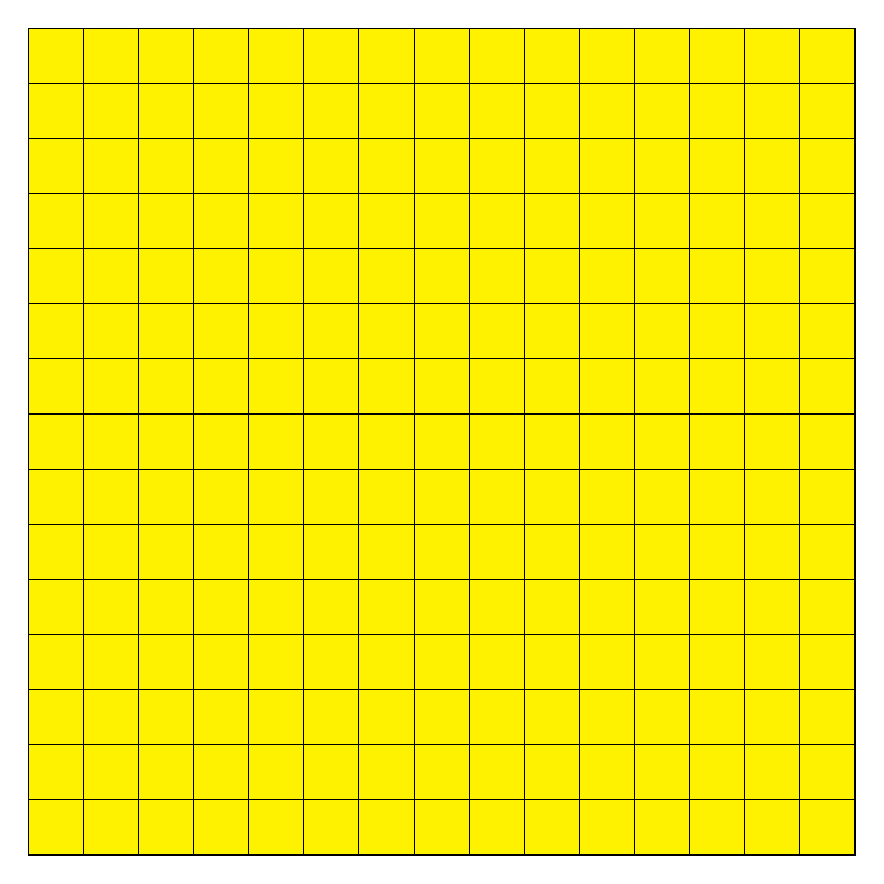
\begin{tikzpicture}[]
\newcommand{\gridsize}{10}
\newcommand{\cellsize}{0.7}

\coordinate (bl) at (0,0);
\coordinate (tr) at (\gridsize,\gridsize);

\foreach \x in {0,\cellsize,...,\gridsize}
	\foreach \y in {0,\cellsize,...,\gridsize}
		\draw [fill=yellow] ($(bl) + (\x,\y)$) rectangle ($(bl) + (\x + \cellsize, \y + \cellsize)$);
		
\emptycell{6}{6}
\emptycell{6}{7}
\emptycell{6}{8}
\emptycell{7}{6}
\emptycell[x]{7}{7}
\emptycell{7}{8}
\emptycell{8}{6}
\emptycell{8}{7}
\emptycell{8}{8}

\end{tikzpicture}
\label{rute:udgangspunkt}
\caption{Udgangspunkt}
\end{figure}


% PART ******************************
\part[Design]{Design\\
	\begin{minipage}[c]{10cm}
	\centering
	\vspace{2cm}
	\normalsize{\textnormal{
		\textit{I denne del beskrives designet af de enkelte elementer, der indgår i projektet. Først beskrives robotten der er brugt til at udføre kortlægning, dernæst den forsøgsopstilling den er blevet brugt i, og til sidst arkitekturen som softwaren på både NXTen og PCen er opbygget omkring.}
	}}
	\end{minipage}
}
\chapter{Robottens design}
Designet af robotten for dette projekt er yderst vigtigt; det er grundstenen i projektet, og uden en velfungerende robot (og specielt kontrol af denne), vil det blive svært at løse problemstillingen for projektet tilfredsstillende.
Dette afsnit fokuserer på hvordan vi er kommet frem til designet af den endelige robot, samt hvilke særlige problemstillinger, der ligger til grund for designet.

\section{Design overvejelser}\label{robot:design}
Designet af robotten har været en del af læringsprocessen for, hvordan man bygger en robot af \lego NXT komponenterne, hvorfor design processen kan ses som en iterativ process, hvor designet er blevet radikalt ændret for hver iteration, indtil et tilfredsstillende resultat er opnået.


\paragraph{Erfaringer fra tidligere designs} 
Der blev konstrueret flere forslag til en robot inden det endelige resultat. 
I dette afsnit vil det blive gennemgået hvilke erfaringer disse initierende designs gav.
I disse forudgående design blev der eksperimenteret med opbygning af en robot med en enkelt ultrasonisk sensor.

\begin{itemize}
\item Hvis NXT enheden fungerer som base med alle andre komponenter monteret på, vanskeliggør det at finde en god placering af robottens ultrasoniske sensor.

\item Hvis sensoren monteres i 1:1 forhold mellem motoren der roterer den, er der alt for store usikkerheder, når sensoren skal roteres x-antal grader (ofte mere end 5\degree).
Disse usikkerheder er et resultat af den manglende præcisionen forbundet med styringen af motoren samt slid af dens interne komponenter, hvilket testes i \cref{sensorer:motorer} også beskriver.
\end{itemize}

\section{Design krav}
Disse to design ledte frem til følgende krav til det endelige design af robotten:
\thilemann{Disse design krav gør sig ikke helt gældende længere. Vi antager bl.a. 90graders verden, hvorfor det ikke er et krav at sensoren kan rotere 360grader.}

\begin{itemize}
\item Den ultrasoniske sensor skal kunne styres med  minimum 1\degree~nøjagtighed, med en foreslået gearing på 1:4.
\item Sensoren(e) skal kunne foretage en 360\degree~måling.
%\item Sekundært indføres der en gearing af hjulene for bedre styring af robotten (nedgearing for højere moment).
\item Mere stabil opbygning for at mindske generelle usikkerheder (bl.a. sidder hjulene bedre fast på basen).
\end{itemize} 


\section{Endeligt design}
Udgangspunktet for det endelige design er baseret på ovenstående design krav sammen med andre idéer, der tilsammen skal øge præcisionen af robotten og gøre den mere driftsikker.

\begin{figure}
\centering
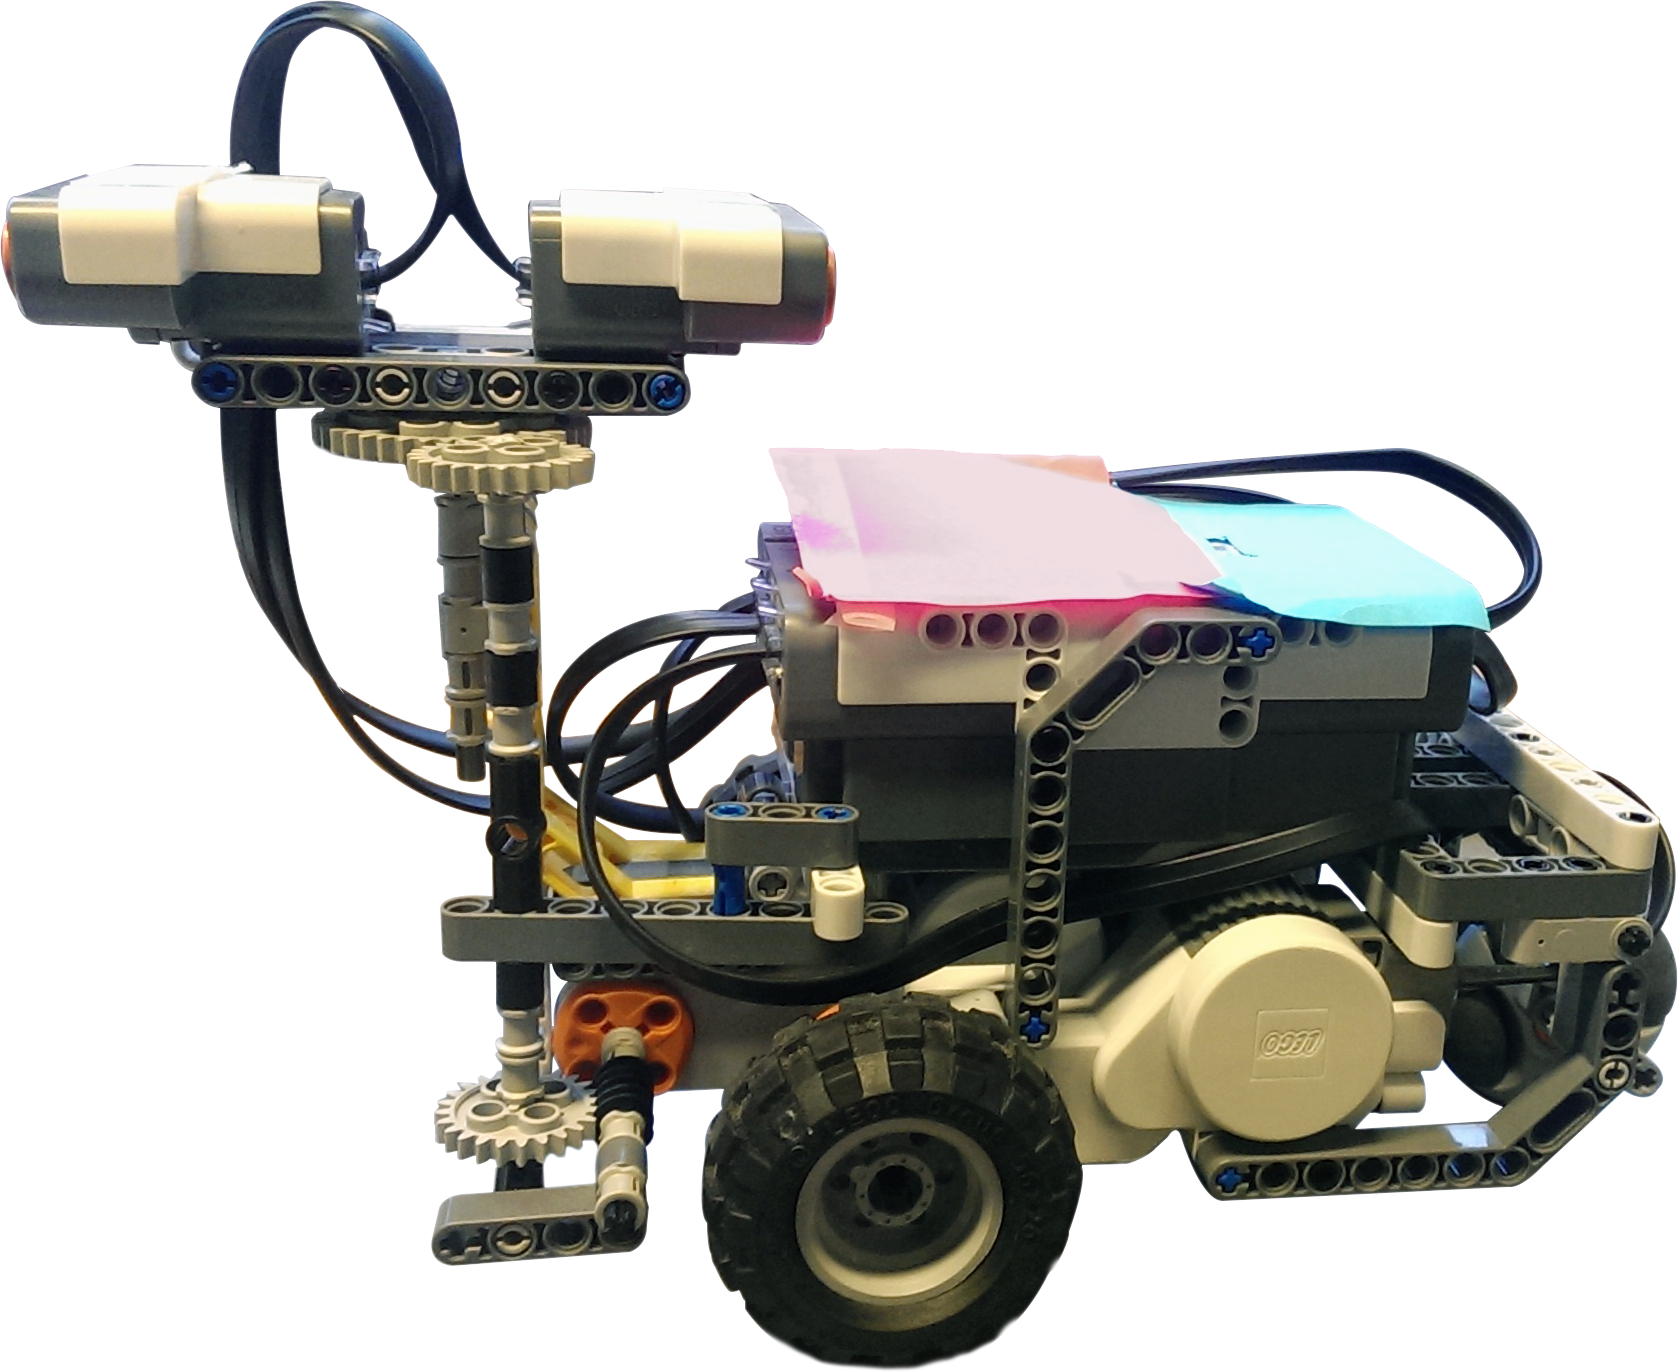
\includegraphics[width=0.6\textwidth]{whalle}
\caption{Endelige design af vores robot.}
\label{robot:opbygning}
\end{figure}

Den vigtigste faktor, når robotten bygges, er placeringen af de primære komponenter, såsom de ultrasoniske sensorer, der skal foretage afstandsmålinger og motoren, der skal skabe fremdrift.

\subsection{Kroppen}
Kroppen er den centrale komponent, der er bygget op omkring motorene som styrer henholdsvis hjulene og rotation af sensorerne. 
Samtidig fungere den som det, der "holder robotten sammen".
Desuden er NXT-enheden også en central del af denne konstruktion.
Placeringen af denne er primært i forhold til funktionelle behov, da der på fronten er knapper til at tænde/slukke og vælge indstillinger med.
Dens placering gør det også nemt at få adgang til dens porte for tilslutning af motor, sensor, opladning samt tilslutning af PC for opdatering af software med mere.

Vigtigt for basen er højden i forhold til armen hvorpå sensorerne er monteret; for at disse skal kunne se i alle retninger er det essentielt at basens relative højde er så lav som muligt i forhold til de ultrasoniske sensorer, således den ikke er i vejen når der f.eks. måles bagud i retningen af basen. 

\subsection{Fremdrift}
Robotten er konstrueret med et \textit{aktivt} hjulsæt, der både giver fremdrift og styring.
Denne funktionalitet opnås ved, at hvert hjul (på hver side af robotten) har sin egen motor, således der kan angives både positiv og negativ fremdrift uafhængigt af hvert hjul.
Dette design gør det muligt at rotere robotten omkring sin egen akse for maksimal mobilitet -- selv på et begrænset område.
Foruden det forreste hjulsæt, er der bagerst på robotten monteret et 'baghjul', hvis eneste funktion er at balancere/stabilisere robotten.
Valget af et hjul til at udføre en sådan funktion er forholdsvis begrænset i \lego, hvorfor valget faldt på et "slæbehjul" med en masse ruller, der gør det muligt for hjulet at rotere i alle retninger.

På de to første design af robotten, var der monteret to store (Ø81,6mm x 15mm) hjul direkte på motorene.
Denne løsning fungerede fint i forhold til højden af basen (og det faktum at robotten stod så godt som vandret), men da gummiet på disse hjul er meget fleksibelt i forhold til sideværts bevægelse (når robotten roterer), blev det vurderet, at det vil give for store usikkerheder ved beregning af rotationen, og at der vil være risiko for at gummiet kan vrides af fælgen med det resultat, at robotten ikke kan køre videre.
\stefan{Skete det, eller er det noget vi bare siger? Hvad er ``en sandsynlighed''?}
\thilemann{Det er vel bare en vurdering af at det kunne ske (har ændret det en smule)}
Derfor er der valgt et lavere og bredere hjulsæt (Ø56mm x 26mm), som er meget mere stabilt.
%Med dette valg samt den højere friktion (større kontaktflade med underlaget), er det valgt at geare motorene der styrer hjulene, hvilket er beskrevet i \cref{robot:gearing}.

\subsection{Sensorer}

\thilemann{Skriver vi før dette at robotten designes med to sensorer? Burde det ikke beskrives før?}
Den egentlige funktion af robotten er at tage afstandsmålinger til objekter indenfor sensorernes rækkevidde.
Placeringen af sensorerne er derfor ikke kritisk, da de højst vil give en forskydelse af konstant faktor relativ til robottens midte fra deres placering i fronten.\thilemann{Skal vi skrive at vi faktisk tager hensyn til dette ved sensormålinger ved at bakke robotten tilbage?}
Vigtigere er, at der er 360\degree~udsyn når de roterer, og at robotten ikke er i vejen for målingerne, hvilket er løst ved at montere sensorerne højere end resten af robotten. 
\thilemann{Der bør nok i subsections laves henvisninger til det kommende billede af robotten}




\section{Gearing}\label{robot:gearing}
I \cref{sensorer:motorer} fandt vi ud af at præcisionen på motorerne ikke var høj.
Der var en afvigelse på op til 4\dg, imod den maksimale afvigelse på 1\dg ~nævnt i kravene i \cref{robot:design}.
Dette faktum gav anledning til at udforske mulighederne for at geare motorene for at mindske usikkerheden og øge præcisionen.

\subsection{Simpel Teori}\label{gearing:simpel_teori}
Gearing kan foregå på to måder; geare op eller geare ned.
Det tandhjul der er knyttet direkte til motoren kalder vi fører-tandhjulet og det tandhjul der er knyttet til fører-tandhjulet kalder vi for følger-tandhjulet (se evt. \cref{gearing:nedgearing}).

\subsubsection{Nedgearing}
Nedgearing foregår ved at et mindre tandhjul driver et større tandhjul.
Gear rationen (størrelsen af gearing) er styret af antallet af tænder på tandhjulene.
For eksempel vil et 24-tands fører-tandhjul drive et 40-tands følger-tandhjul med ratioen $1:1.667$, hvilket betyder at der for at give en enkelt følger omdrejning kræves $1.667$ fører omdrejninger. 
Det betyder at motoren der driver fører-tandhjulet skal rotere $\frac{40}{24} = 1 \frac{2}{3}$ omgange for at rotere følger-tandhjulet én omgang og at følger tandhjulet roterer $\frac{1}{1.667} = 0.6$ omgange pr. omdrejning af fører tandhjulet.

Til dette projekt bliver der kun gearet ned (jævnfør robottens design på \cref{robot:opbygnin}); dette gør sig gældende for begge sæt af gearinger.


\begin{figure}[h]
\centering

\includegraphics[width=.5\textwidth]{gears/op_og_ned}
\caption{Eksempel på (ned-)gearing}
\label{gearing:nedgearing}
\end{figure}

\subsection{Aktuelle gearing}
Dette afsnit fokuserer på den teoretiske gearing for de ultrasoniske sensorer.
\Cref{robot:gearing-test} beskriver forskellige test af gearingerne der driver sensor rotationen for at undersøge om gearingen lever op til de teoretiske værdier.


\subsubsection{Ultrasonisk sensor}
Denne bruges til at bestemme afstanden til et objekt i en bestemt retning, hvorfor det vil være en fordel at geare motoren ned for at opnå større præcision af denne når retningen af sensoren skal bestemmes.
Rotationen vil naturligvis foregå langsommere end uden gearing, men da tid ikke er en faktor på nuværende tidspunkt er det ikke af nogen betydning for at løse problemet.

Gearingen for den ultrasoniske sensor består af i alt 3 forskellige tandhjul (4 i alt), som alle kan ses i \cref{gearing:tandhjul}.

\begin{figure}[h] % De anvendte tandhjul
\centering
\begin{subfigure}[b]{.19\textwidth}
\centering
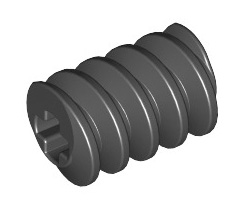
\includegraphics[width=\textwidth]{gears/worm}
\caption{Snekke}
\label{gearing:snekke}
\end{subfigure}
%\begin{subfigure}[b]{.19\textwidth}
%\centering
%
\includegraphics[width=\textwidth]{gears/16-tooth}
%\caption{16-tands}
%\label{gearing:16tand}
%\end{subfigure}
\begin{subfigure}[b]{.19\textwidth}
\centering

\includegraphics[width=\textwidth]{gears/24-tooth}
\caption{24-tands}
\label{gearing:24tand}
\end{subfigure}
\begin{subfigure}[b]{.19\textwidth}
\centering

\includegraphics[width=\textwidth]{gears/40-tooth}
\caption{40-tands}
\label{gearing:40tand}
\end{subfigure}
\caption{De anvendte tandhjul til sensor rotation}
\label{gearing:tandhjul}
\end{figure}

Den første kombination består af en snekke\cite{snekke} (se \cref{gearing:snekke}) som fører-tandhjul og 24-tands (se \cref{gearing:24tand}) som følger-tandhjul.
Snekken kræver en hel rotation for at flytte én tand på følger-tandhjul giver en gear ratio på $1:24$, hvilket betyder at der kræves 24 hele motor-rotationer for at rotere 24-tands (følger) tandhjulet én omgang.

Den anden kombination består af et 24-tands (se \cref{gearing:24tand}) som fører-tandhjul og et 40-tands (se \cref{gearing:40tand}) som følger-tandhjul, hvilket giver en ratio på $1:1.667$.

Den samlede gear ratio for sensor motoren bliver derfor $1:40$, som beskriver at der for hver sensor omdrejning kræves 40 motor omdrejninger; hvilket er det samme som:
$$\frac{24}{1} \cdot \frac{40}{24} = 40$$

\subsection{Test af gearing}\label{robot:gearing-test}
\thilemann{Jeg mener vi bør udføre testene igen og notere resultaterne således de kan komme i appendix sammen med de andre test resultater - de mangler lidt som argumentation i testen beskrevet herunder.}
Nu hvor den teoretiske gearing er fastlagt, vil der her blive udført en række forsøg for at afgøre præcisionen af sensor motoren med gearing; og evt. at fastlægge en faktisk gearing, hvis denne afviger fra den teoretiske.

\subsubsection{Sensor}
Det er vigtigt at kende den nøjagtige rotation af sensoren, og dermed dens retning, for at få så præcise målinger som muligt.
Derfor er der foretaget to forskellige test, hvis formål er at kortlægge eventuelle usikkerheder der kan være indført med gearing af sensor motoren.

\paragraph{Første test} var en grovtest, hvor der blev kørt i den samme retning i et antal sensor-omdrejninger.
Der blev udført handling med sensor-omdrejninger som input, ud fra en beregnet motor-omdrejning, baseret på den teoretiske gearing.
Denne test gav et godt resultat, uden afvigelse.
\thilemann{en forsker udførte engang en meget hemmelighedsfuld test af en gearing helt ude i skoven, uden nogen former for resultater...}

\paragraph{Anden test} blev udført ved at køre færre omdrejninger, skiftevis med og mod uret.
Dette gav en upræcision, da der er slør i den øverste gearing mellem 40-tands og 24-tands tandhjulene.
Dette slør giver mellem $\frac{1}{4}$ og $\frac{3}{4}$ tands unøjagtighed, da der ved skift af rotations-retning bruges op til $\frac{3}{4}$ tandhjul-omdrejning for 24-tands tandhjulet at få fat i 40-tands tandhjulets tænder igen.
\chapter{Forsøgsopstilling}
\section{Testmiljø}
I dette afsnit præsenteres testmiljøet der sat op til at teste robottens færdigheder.

\subsection{Formål}
Formålet med et testmiljø er for bedre at kunne kontrollere omgivelserne.
Dette giver mindre unøjagtigheder ifht. hvis det skulle testes i et nyt miljø hver gang og muligheden for at sammenligne resultater.

\subsection{Opsætning}\label{testmiljo:opsaetning}
Testmiljøet er opsat vha. papkasser og tape, som man kan se på \cref{testmiljo:perspektiv}.
Størrelsen er $189 \ cm \times 261 \ cm$ grunden til denne størrelse er at dette præcis passer ifht. kinectens billede som man kan se på \cref{testmiljo:oppefra}.
På \cref{testmiljo:forfra} kan man se hvordan kinecten er monteret under en loftplade.

\begin{figure}
\begin{tikzpicture}
\node[anchor=south west,inner sep=0] at (0,0) {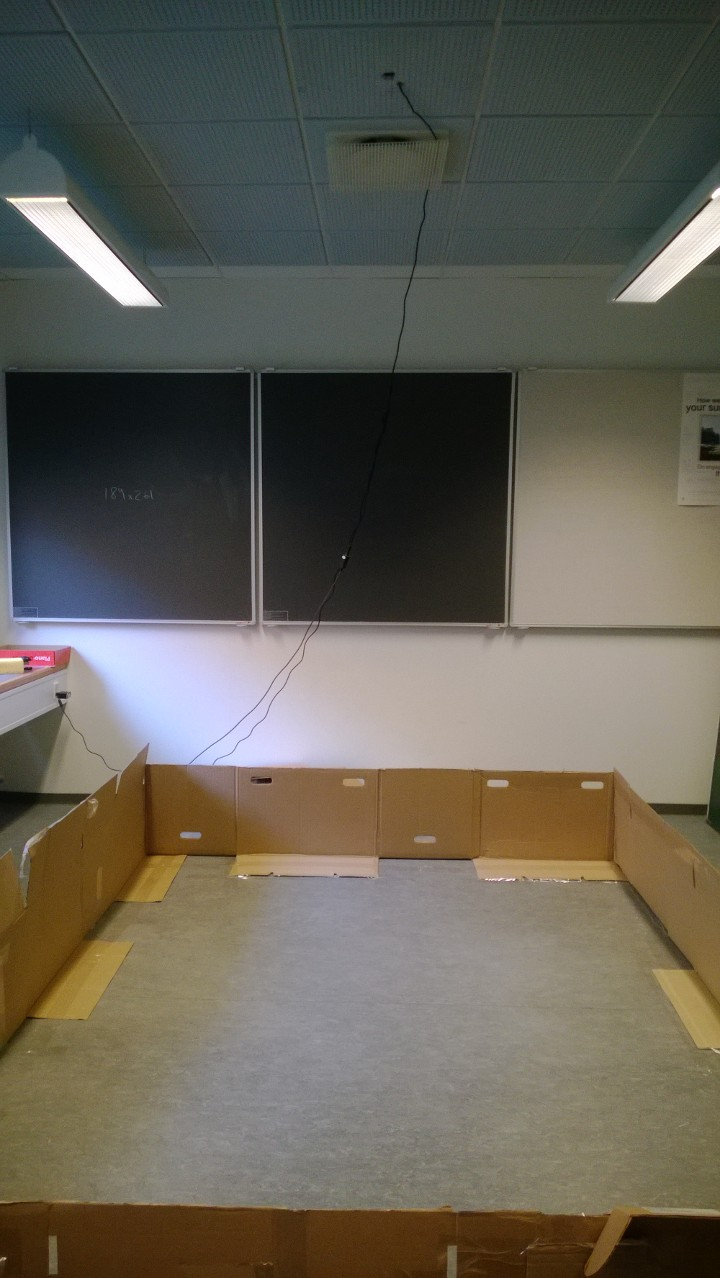
\includegraphics[width=\textwidth/2]{./verden/forfra}};
    \draw [->, red, ultra thick] (5.5,10.5) -- (4.2,11.2);
\end{tikzpicture}
\caption{Testmiljøet set forfra. Bemærk kinecten monteret i en loftplade(rød pil) med hul til RGB-kameraet.}
\label{testmiljo:forfra}
\end{figure}

\begin{figure}
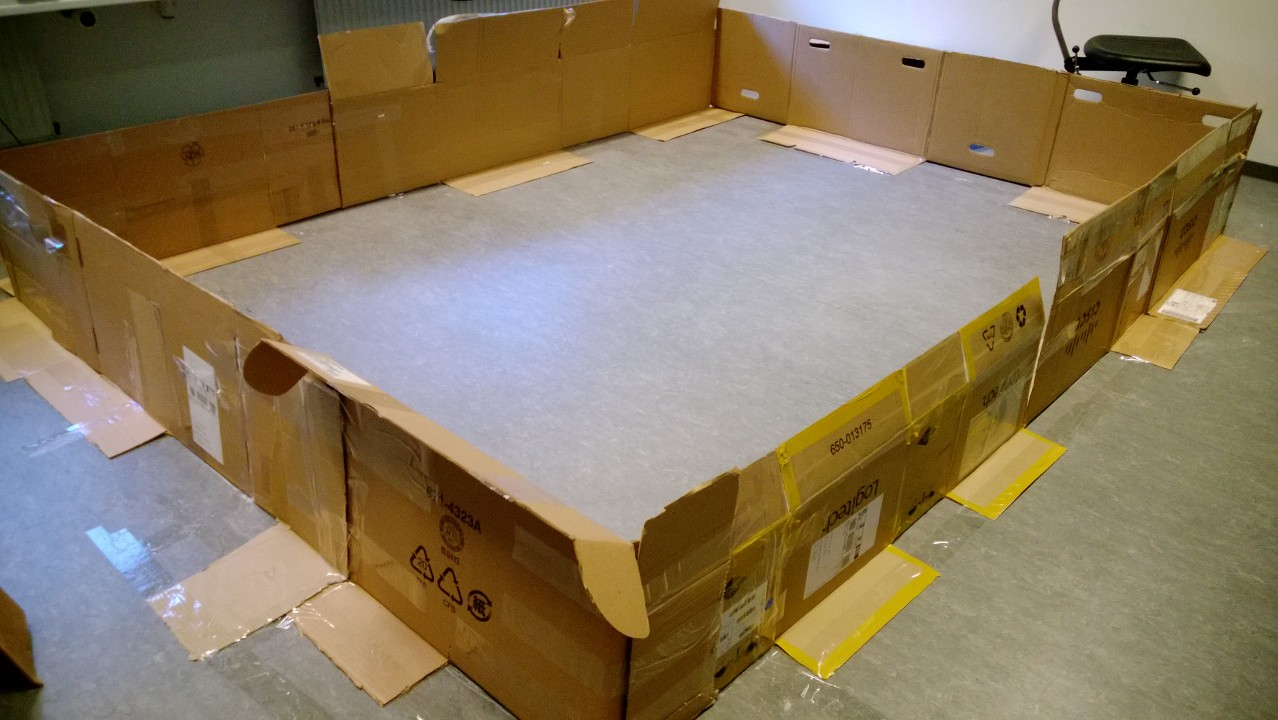
\includegraphics[width=\textwidth]{./verden/perspektiv}
\caption{Testmiljøet set i perspektiv.}
\label{testmiljo:perspektiv}
\end{figure}

\begin{figure}
\begin{tikzpicture}
\node[anchor=south west,inner sep=0] at (0,0) {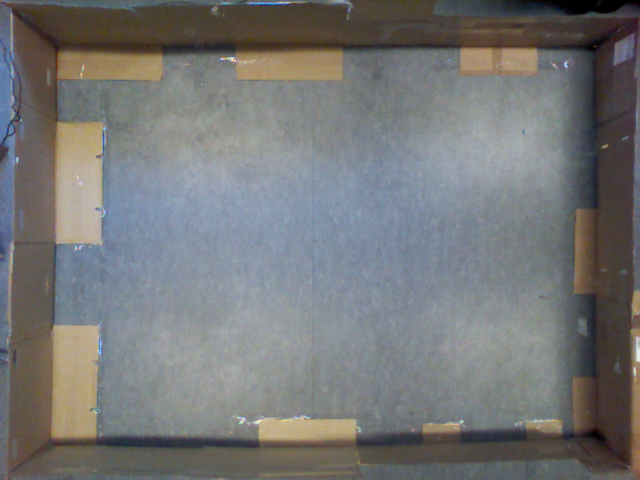
\includegraphics{./verden/oppefra}};
    \draw [<->, red, ultra thick] (1.3,0.9) -- (1.5,11.4);
    \node [red, ultra thick] at (2.5,5.5) {189 cm};
    \draw [<->, red, ultra thick] (1.3,0.9) -- (16,1);
    \node [red, ultra thick] at (8, 2) {261 cm};
\end{tikzpicture}
\caption{Testmiljøet set fra kinecten.}
\label{testmiljo:oppefra}
\end{figure}
\chapter{System Arkitektur}
% !TeX spellcheck = da_DK
Dette kapitel vil beskrive systemets arkitektur.
Systemet er delt i to dele, én på computeren og en på NXTen.


\begin{figure}[H]
\centering
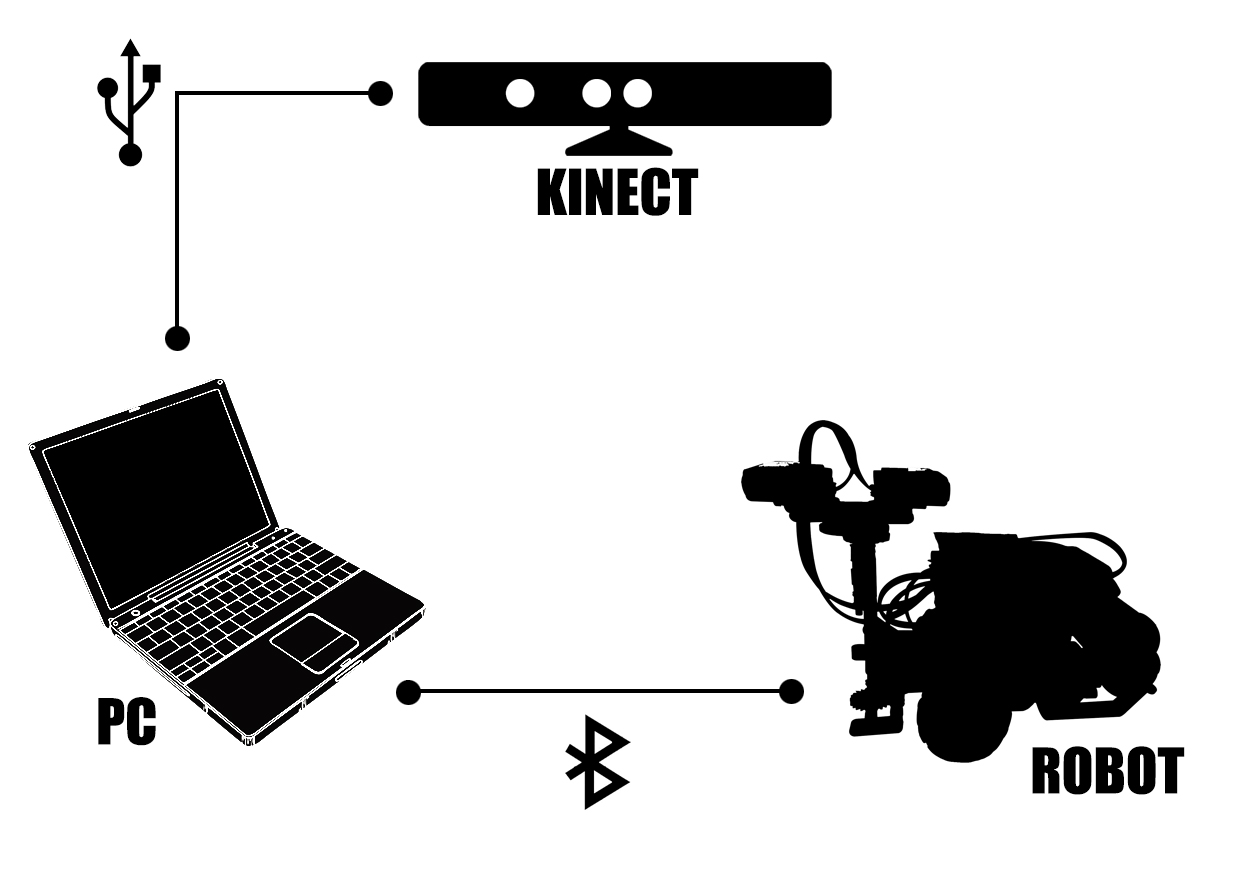
\includegraphics[width=1.0\textwidth]{enheder}
\caption{Systemets opbygning}
\label{arkitektur:opbygning}
\end{figure}

Den overordnede opbygning af systemet kan ses på \cref{arkitektur:opbygning}.
Selve kortlægningen sker på computeren hvor occupancy grid algoritmen køres.
Computeren får sine oplysninger fra robotten gennem en bluetooth forbindelse.
Computeren bruger det grid der er konstrueret til at fortælle robotten hvor den skal køre hen.
Computeren hjælper robotten med at fortælle den hvor den er ved at fortolke et billede fra Kinecten og sende denne oplysning til robotten hver gang den beder om det.
Når robotten er kommet frem til et punkt foretager den en sensormåling og sender denne tilbage til computeren.

I de følgende afsnit vil arkitekturen på henholdsvis NXTen og computeren blive beskrevet.


% !TeX spellcheck = da_DK
\section{NXC arkitektur}
Koden der kører på robotten er bygget op omkring et modul der hedder MotorControl. \cite{MotorControl}
MotorControl er et program der kører på NXTen og sørger for at motorerne kører præcis den afstand de bliver bedt om. 
Uden MotorControl er motorerne meget upræcise hvilket gør det svært at navigere robotten til et bestemt sted.

Da der kun kan køre ét program ad gange på NXTen indeholder vores program en modificeret version af MotorControl, hvor alle navigationsfunktioner udnytter MotorControl.

Koden på robotten er opdelt i filer efter hvilket ansvar de har.
I det følgende vil hver fil blive beskrevet.

\subsection{MotorControl}
For at MotorControl kan fungere er der inkluderet følgende filer der ikke er ændrede i forhold til kilden.

\begin{itemize}
\item \textbf{SpeedFromPosLookup.nxc}
\item \textbf{MotorFunctions.nxc}
\item \textbf{ControllerCore.nxc}
\item \textbf{Controller.nxc}
\end{itemize}

Filen \textbf{MCTasks.nxc} indeholder de tasks der er i den originale MotorControl med ændringer der gør dem brugbare i vores program.
Den indeholder desuden en \lstinline[style=c]!Run! metode som sætter MotorControl igang. 
Denne Run funktion var i det originale MotorControl en del af et switch statement i \lstinline[style=c]!Main! funktionen, og er derfor trukket ud så det er en funktion der kan kaldes.

\subsection{NXC koden}

Programmet samles i filen \textbf{MainTask.nxc} som indeholder hovedloopet. 
I dette loop venter robotten på komandoer fra computeren og reagerer derefter på dem.

Alt hvad robotten skal gøre håndteres i en af disse tre filer

\begin{itemize}
\item \textbf{Navigation.nxc}
\item \textbf{Sensor.nxc}
\item \textbf{Communication.nxc}
\end{itemize}

\textbf{Navigation.nxc} styrer robottens generelle navigation, for eksempel \lstinline[style=c]!RunForward! der beder robotten køre fremad, \lstinline[style=c]!TurnAngle! der drejer robotten og \lstinline[style=c]!GoToPoint! der beder robotten køre hen til et bestemt punkt.
Filen \textbf{Sensor.nxc} bliver brugt hver gang der skal foretages en sensormåling, og filen \textbf{Communication.nxc} bliver brugt til at kommunikere med computeren med funktionerne \lstinline[style=c]!IAmThere! når robotten har nået sin destination og funktionen \lstinline[style=c]!WhereAmI! når robotten forespørger sin position.

\thilemann{Dette hænger ikke så godt sammen med forrige afsnit om nxc arkitektur.}
\label{arkitektur}
\section{Computer Arkitektur}
Til dette projekt er det besluttet at bygge systemet efter en lag-delt struktur.
Denne beslutning er taget for at overkomme kompleksiteten af systemet; altså for at give hvert gruppemedlem bedre overblik over koden, men også for at skabe nogle generelle retningslinjer for placering af dets komponenter.

I de efterfølgende afsnit vil arkitekturen (som ses på  \cref{arkitektur:klassediagram:1,arkitektur:klassediagram:2}) blive beskrevet.
Beskrivelsen vil fokusere på hvad de enkelte lag (namespaces) har til formål, samt hvordan lagene interagerer med hinanden.
Som det også ses på figurerne, er det kun de ydre associationer, der er angivet for at simplificere beskrivelsen af systemet.
Som det første beskrives \lstinline[style=csharp]!CommonLib.dll! i \cref{arkitektur:commonlib}, da systemets lag alle holder referencer hertil.
Efterfølgende vil lagene blive beskrevet i en rækkefølge, der følger kaldene internt i systemet.
\begin{figure}
\centering
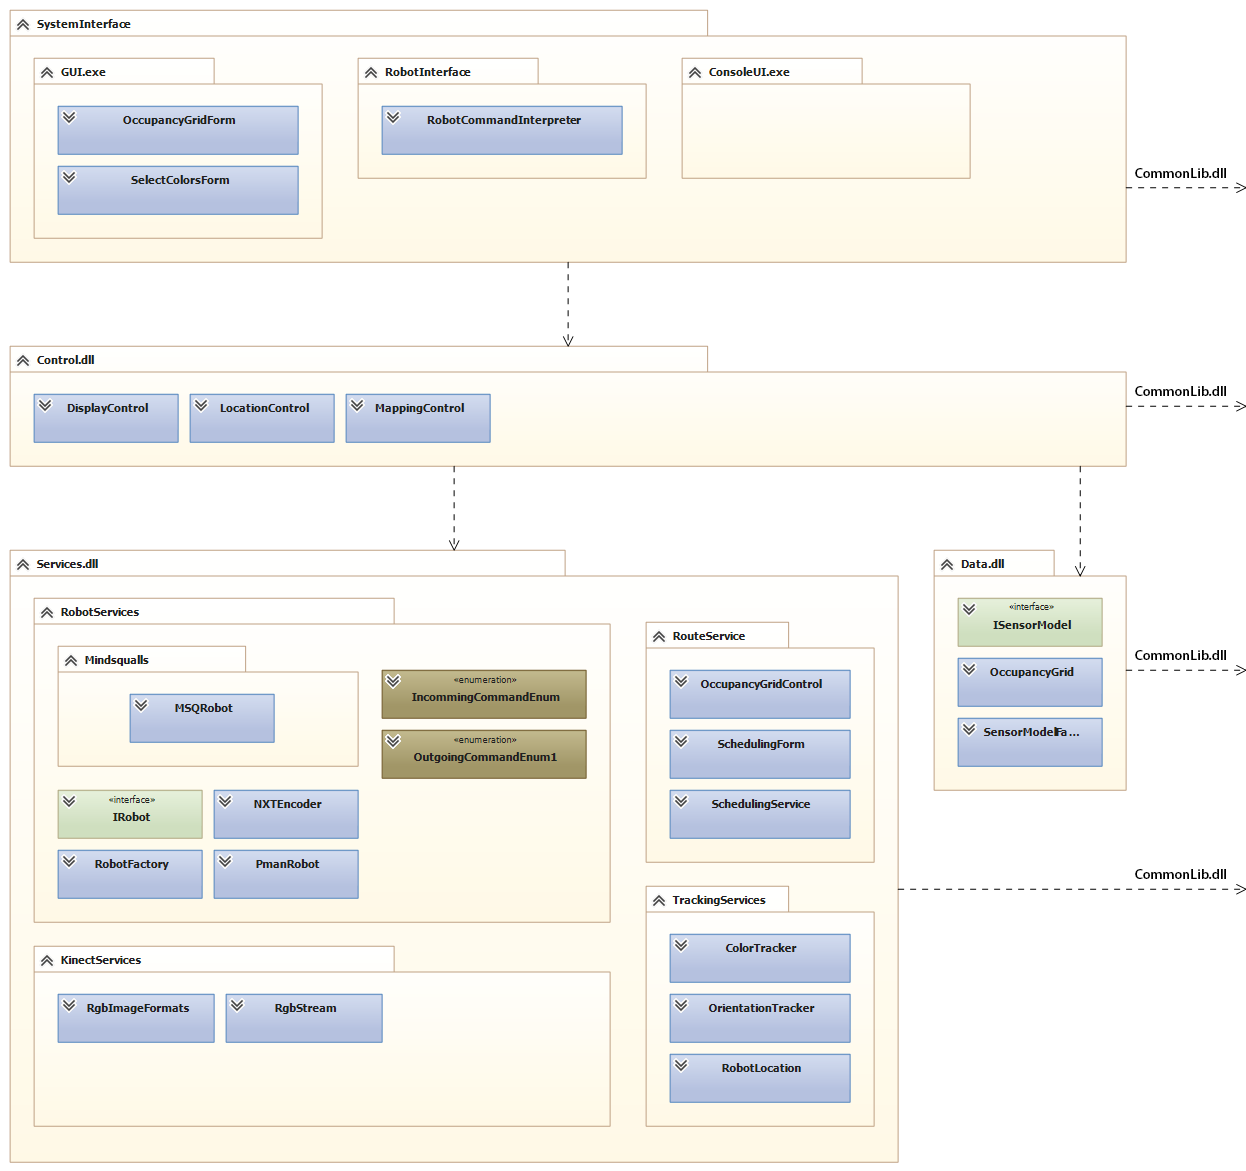
\includegraphics[width=1\textwidth]{./graphics/systemarkitektur_1}
\caption{Lagene i systemarkitekturen med deres ydre associationer. Associationerne til højre fører alle til \lstinline[style=csharp]!CommonLib.dll!, som ses på \cref{arkitektur:klassediagram:2}.}
\label{arkitektur:klassediagram:1}
\end{figure}

\begin{figure}
\centering
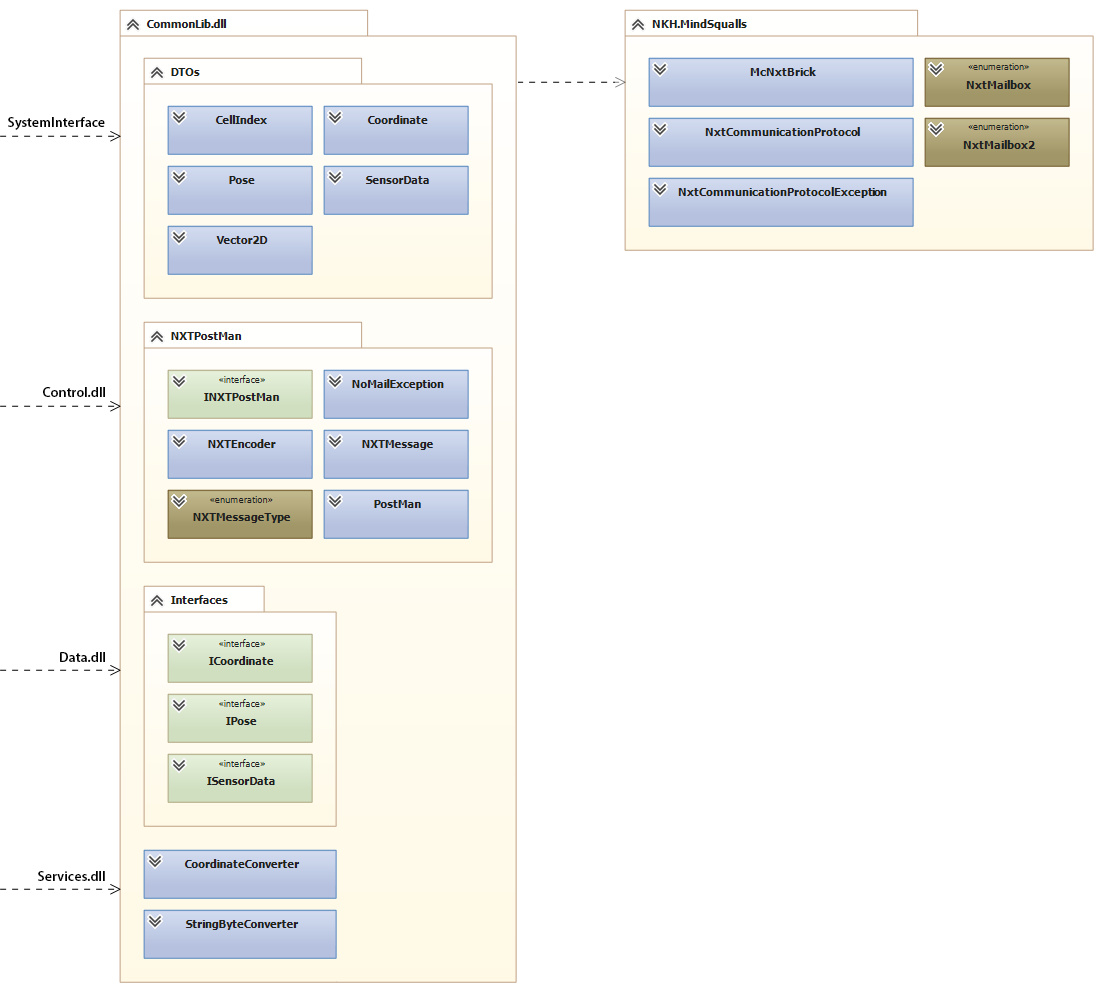
\includegraphics[width=1\textwidth]{./graphics/systemarkitektur_2}
\caption{Viser namespacet \lstinline!CommonLib.dll! (uden interne associationer), som er en del af den lagdelte systemarkitektur. De fleste lag i arkitekturen har associationer til netop \lstinline!CommonLib.dll!, der indeholder de elementer, som benyttes af alle lag. De refererende namespaces kan ses på \cref{arkitektur:klassediagram:1}.}
\label{arkitektur:klassediagram:2}
\end{figure}
\section{CommonLib.dll}\label{arkitektur:commonlib}
Benyttes af alle lag i arkitekturen.
Dets formål er at samle de komponenter som i systemet kan benyttes af alle lag.
Derfor holder det også en reference til namespacet \lstinline[style=csharp]!NKH.MindSqualls! for at kunne tilgå den del af MindSqualls (\cref{mindsqualls}) som indeholder kommunikationen til NXT-enheden.

\paragraph{CommonLib.DTOs}
Dette namespace indeholder alle \textit{Data Transferring Objects} som har til opgave at sende data mellem de forskellige lag.

\paragraph{CommonLib.NXTPostMan}
Som navnet på namespacet antyder, så er formålet med \lstinline[style=csharp]!CommonLib.NXTPostMan! at sende beskeder frem og tilbage mellem PC og robotten; hvilket gør det ansvarlig for al kommunikation imellem de to, som beskrives detaljeret i \cref{kommunikation}.

\paragraph{CommonLib.Interfaces}
Definerer en række interfaces, som implementeres af de respektive DTO'er.
Dette minimerer koblingen af koden og gør dem samtidig mere modulær, da komponenter nemt kan udskiftes.

\section{NKH.MindSqualls}\label{arkitektur:mindsqualls}
Dette er koden fra MindSqualls frameworket (beskrevet i \cref{mindsqualls}).
Det er dog ikke alle komponenter i frameworket der benyttes; det benyttes primært til at etablere kommunikation mellem NXT-enheden og PC samt exceptions, hvilket implementeres gennem \lstinline[style=csharp]|PostMan| klassen.

\section{SystemInterface}\label{arkitektur:systeminterface}
Dette er "indgangen" til systemet og er derfor også den komponent, som er ansvarlig for alle ydre påvirkninger; det være sig f.eks. brugerinput eller andre systemer, som ønsker at tilgå systemet.

\paragraph{SystemInterface.GUI.exe}
Dette namespace indeholder de grafiske komponenter for systemet, og er derfor programmet, der starter systemet.
Det er ansvarlig for at modtage og reagere på brugerens input.

\paragraph{SystemInterface.RobotInterface}
Essensen i dette namespace er en tråd, der konstant tjekker efter nye beskeder på NXT-enheden.
Den benytter så henholdsvis \lstinline[style=csharp]|LocationControl| og \lstinline[style=csharp]|MappingControl| til at reagere på beskeder den finder, og anmoder dermed \lstinline[style=csharp]!Services! namespacet om at udføre den pågældende handling.

\section{Control.dll}\label{arkitektur:control}
Denne komponent i arkitekturen er ansvarlig for kontrol af robotten samt opdatering af data.
Kald hertil stammer fra \lstinline[style=csharp]!SystemInterface!, der anmoder om en action, som dette namespace så reagerer på ved at benytte \lstinline[style=csharp]!Services! namespacet.

\paragraph{Control.DisplayControl}
Er en klasse som henter en videostrøm fra farvekameraet på en Microsoft Kinect.

\paragraph{Control.LocationControl}
Denne klasse opdaterer lokationen af robotten.
Den indeholder således også information om robottens omgivelser og robotten selv.

\paragraph{Control.MappingControl}
Al kontrol af robotten på kortet (occupancy grid) foregår gennem denne klasse.
Den indeholder således metoder til at sende robotten til et nyt koordinat, opdatere kortet og hente nye sensormålinger.

\section{Services.dll}\label{arkitektur:services}
Dette er det nederste lag i arkitekturen og benyttes af \lstinline[style=csharp]!Control! namespacet når en handling ønskes udført.

\paragraph{Services.RobotServices}
Dette namespace benyttes, når robotten skal kontrolleres.
Det er således herigennem, der sendes beskeder til robotten, for at få den til at bevæge sig til en ny position og tage sensormålinger.

\paragraph{Services.RouteService}
For at få robotten til at køre en rute på kortet benyttes \lstinline[style=csharp]!RouteService! namespacet, der består af en grafisk komponent, der gør det muligt at klikke en rute ind på et occupancy grid samt en \lstinline[style=csharp]|SchedulingService|, der returnerer en kø af de punkter, som ruten består af.

\paragraph{Services.KinectServices}
Benyttes af \lstinline[style=csharp]!Control.DisplayControl! for at vise en videostrøm fra farvekameraet i Kinecten.
Konverterer den returnerede videostrøm til en strøm af bitmaps, som kan vises grafisk i \lstinline[style=csharp]!SystemInterface!.

\paragraph{Services.TrackingServices}
Denne service er ansvarlig for at holde styr på robottens lokation samt positur.
Robotten kan således gennem \lstinline[style=csharp]!Control! benytte dette namespace, når den ønsker en opdatering af sin positur.

\section{Data.dll}\label{arkitektur:data}
Dette assembly indeholder alle data objekter for occupancy grid samt sensormodellen.
Alt data opdateres fra \lstinline[style=csharp]!Control! når robotten har taget en ny måling.







\section{Kommunikationsprotokol}\label{kommunikation}
% !TeX spellcheck = da_DK

Dette afsnit beskriver kommunikationen mellem NXT og computer.
Afsnittet beskriver de beskeder der bliver sendt frem og tilbage og de indkodes inden de sendes.

\subsection{Besked}
Beskeder vil i dette afsnit beskrives ved brug af vinklede parenteser til at indikere dele af beskeden.
En besked er opbygget på følgende måde:
\begin{equation}
<BeskedType><Indhold>
\end{equation}
Beskedens type indkodes som strengrepræsentationen af typenummeret.
Dette tal er enten en eller to bytes.
Beskeder på én byte sendes fra robotten og modtages af computeren mens beskeder på to byte sendes fra computeren og modtages af robotten.
Beskedindholdet består af ingen eller flere bytes.
I det næste afsnit vil de forskellige beskeder der benyttes blive beskrevet.

\subsection{Besked typer}
Alle beskederne kan ses i \cref{design:protokol_tabel}.
\\
Første kolonne fortæller hvilken talkode der benyttes til at indikere beskedens type.
Anden og tredje kolonne fortæller henholdsvis om beskeden går fra computerens eller NXT'ens inbox eller outbox.
De to sidste beskriver hvad beskeden indeholder og gør.
Nedenfor er de forskellige scenarier som beskederne fra tabellen bliver brugt, samt en uddybning af indkodningen af beskedindholdet.


\begin{figure}[H]
\renewcommand{\arraystretch}{1.8}
\begin{longtable}{ c | c | c | p{0.4\textwidth} | c}
Besked type & Computer & NXT & Beskrivelse & Indhold\\
\hline
\hline
0 & IN & OUT & Robotten forespørger om dens lokation & - \\
1 & IN & OUT & Robotten er nået frem til dens lokation & - \\
2 & IN & OUT & Robotten sender sensordata & $s1_x,s2_x,s1_y,s2_y$ \\
50 & OUT & IN & Computeren fortæller roboten at den skal bevæge sig til en position  & $x,y$\\
51 & OUT & IN & Computeren beder om at få sensor data fra robotten & - \\
52 & OUT & IN & Computeren sender robottens position til robotten & $x,y,a$\\
\hline
\caption{Oversigt over de forskellige beskeder}\label{design:protokol_tabel}\\
\end{longtable}

\end{figure}

\subsubsection{Nuværende lokation}\label{protokol:positur}
Denne situation forekommer når robotten skal bede om sin lokation fra computeren.
Robotten sender en besked på formen 
\[
< \! ''0'' \! >
\]


Derefter returnerer computeren en besked på formen
\[< \! ``52'' \!><x><y><a>\]
Denne besked indeholder lokationen og dens vinkel hvor $x$ og $y$ repræsenterer lokationen og $a$ vinkelen.
Koordinaterne fortolkes i et koordinatsystem med millimeter på akserne.
Værdierne indkodes som koordinatværdierne repræsenteret som en streng på 7 tegn.
Der tilføjes nuller til venstre for tallet hvis tallet er 7 tegn.
Vinklen fortolkes som vinklen mellem x-aksen og en linje fra (0,0) til robotten.
Ligesom koordinaterne indkodes vinklen som strengrepræsentationen af vinklen på 7 tegn.

\subsubsection{Naviger til en ny lokation}\label{design:protokol_navigertilny}
Denne situation opstår når computeren sender en besked der fortæller robotten hvor den skal køre hen.

computerens besked er på formen
 \[<\! ''50'' \!><x><y>\] 
hvor $x$ og $y$ er koordinaterne til det punkt robotten skal køre hen til.
Koordinaterne fortolkes i et koordinatsystem med millimeter på akserne.
Værdierne indkodes som koordinatværdierne repræsenteret som en streng på 7 tegn.
Der tilføjes nuller til venstre for tallet hvis tallet er 7 tegn.

\subsubsection{Nået frem til lokation}
Denne situation forekommer når robotten er nået frem til den ønskede lokation.
Robotten sender da en besked på formen \[<\!''1''\!>\]

\subsubsection{Aflæs Sensordata}
Når computeren beder om sensor data fra robotten, sender den en besked på formen \[<\!''51''\!>\]
Robotten foretager derefter sensormålinger og returnerer dem med en besked på formen  
\[<\!''2''\!><s1_x> <s2_x> <s1_y> <s2_y>\]
Sensordata består af en måling fra hver sensor før sensorerne roterer 90 grader og efter.
$ s1_x $ og $ s2_x $ er derfor to målinger mens sensorerne står i startpositionen, mens $ s1_y $ og $ s2_y $ er to måling efter sensorerne er drejet 90 grader.
Sensormålingerne sendes hver som én byte.
\section{Flow- og Kodeeksempel}

Robot vil vide hvor den er:
\begin{enumerate}
\item Robot lægger besked OUTGOING\_WHERE\_AM\_I i outbox
\item Robotten går i gang med kontinuerligt at checke sin inbox efter beskeden INCOMING\_GET\_POS
\begin{enumerate}
\item Hvis beskeden er der:\\
Opdater robottens pose med den der ligger i inbox
\item Ellers:\\
Check efter besked
\end{enumerate}
\item RobotInterface beder kontinuerligt Postman om at checke inbox (Robottens outbox)
\begin{enumerate}
\item Hvis der er besked og denne er RobotRequestsLocation:\\
Bed LocationControl om robottens pose
\item Hvis der er besked og den ikke er RobotRequestsLocation:\\
Udfør den anden handling
\item Ellers:\\
Check efter besked
\end{enumerate}
\item LocationControl beder RobotLocation i TrackingServices om robottens pose
\item RobotInterface beder Postman om at lægge robottens pose i outbox (Robottens inbox)
\item Der var besked i robottens inbox
\end{enumerate}

% PART ******************************
\part[Konklusion]{Konklusion\\
	\begin{minipage}[c]{10cm}
	\centering
	\vspace{2cm}
	\normalsize{\textnormal{
		\textit{Denne del er den afsluttende del af rapporten.
		Der vil først blive givet resultater for de udførte tests, samt evaluering af disse ud fra målsætningen.
		Slutteligt vil der blive konkluderet og perspektiveret over resultaterne, med forslag til fremtidige forbedringer.}
	}}
	\end{minipage}
}
\chapter{Evaluering}
Dette kapitel evaluerer de to valgte sensormodeller(\cref{mapping:sensormodel}) og ruteplanlægning(\cref{ruteplanleagning}).


\section{Formål}
Formålet med denne test er at se hvilken sensormodel der kommer frem til det mest præcise kort og hvilken indvirkning ruteplanlægningen har.

\section{Test}\label{evaluering:test_beskrivelse}
Der bliver foretaget tre tests med hver sensormodel(\cref{mapping:sensormodel}).
I alle test benyttes ruteplanlægning beskrevet i \cref{ruteplanlaegning}.
Startpositionen er altid den samme.
Robotten kører hen til et punkt og scanner to gange - dette foretages 75 gange.
Alle data bliver logget så det er muligt at genskabe et kort udfra det.

\subsection{Opstilling}

\subsection{Resultater}

\subsection{Opsummering}
\chapter{Opsummering}
\chapter{Perspektivering}
% !TeX spellcheck = da_DK
Projektets resultater kan som altid forbedres.\thilemann{i forhold til hvad? synes det virker lidt dumt at skrive.}
Nogle elementer er bevidst ikke implementeret på grund af tidsbegrænsning, og andre er gruppen kommet frem til, givet de erfaringer der er gjort i løbet af projektet.

I dette afsnit præsenteres forslag til mulige forbedringer af systemet, samt en vurdering af hvor anvendeligt det endelige produkt er.

\section{Lokalisering}
Kinecten brugt til lokalisering fra starten af projektet, da det var meningen at bruge dybdesensoren til at lokalisere objekter i et billede.
Siden da blev løsningen ændret til at genkende objekter ved farve, men Kinecten blev beholdt.
Det ville derfor være muligt at udskifte Kinecten med et almindeligt webcam, som ville være lettere at komme i besiddelse af. 
Der er også et større udvalg af webcams, så det vil være muligt at finde en bedre opløsning, opdateringshastighed eller en anden parameter der vil forbedre lokaliseringen.
\thilemann{Undskyld... Men jeg synes ikke ovenstående afsnit er særligt godt skrevet :(}

\section{Implementering}
I dette projekt er der blevet implementeret to forskellige sensormodeller. \stefan{indsæt vurdering af de to modeller}
En forbedring ville være at implementere endnu bedre sensormodeller.\thilemann{giver det ikke lidt sig selv?}

I de udførte test er der benyttet en cellestørrelse på 10cm $ \times $ 10cm.
Denne cellestørrelse blev valgt med henblik på at gøre cellerne så små som muligt, uden at tiden det ville tage at kortlægge området ville blive alt for stor.
Man kunne således forsøge at variere størrelsen af celler for at finde ud af hvilken indvirkning det har på resultaterne.

Allerede i problemformuleringen blev robottens verden afgrænset til kun at være 90 grader. 
Denne afgrænsning gjorde nogle aspekter af problemer lettere. 
Blandt andet simplificerede det den måde sensormålinger skal behandles når occupancy griddet skal opdateres.
En forbedring ville være at ophæve denne begrænsning så der kan tages målinger i 360 grader.

Ved test af systemet blev det bemærket at der blev brugt en del tid på at robotten flyttede sig fra et punkt til et andet.
I dette tidsrum blev der ikke foretaget nogle målinger og var derfor 'spildt' tid. 
Dette kunne forbedres ved at robotten tog løbende målinger, så tiden brugt mellem to punkter blev mere effektivt udnyttet.

\section{Robotkonstruktion}
Robotten er blevet konstrueret med to sensorer der kan dreje. 
Således er det muligt at tage en sensormåling forud og bagud, og derefter dreje sensortårnet til at tage sensormålinger til begge sider.
Dette har vist sig at være unødvendigt, da tiden det tager at dreje tårnet gør det upraktisk.
Det viste sig også at komplicere registreringen af sensormålinger, da sensortårnet ikke kunne placeres lige over det punkt der blev brugt til at lokalisere robotten.
En ændring af dette kunne være at fastmontere sensorerne og nøjes med at dreje robotten.
Et andet alternativ vil være at montere 4 sensorer i stedet for to, så det slet ikke vil være nødvendigt at dreje hverken et sensortårn eller robotten for at tage målingerne.

Ved konstruktionen af systemet blev det antaget at ruteplanlægningen skulle have ansvaret for at robotten ikke kører ind i noget. 
Dette gøres ud fra det occupancy grid der ind til videre er konstrueret.
Det viste sig dog til nogle af de indledende prøvekørsler at dette ikke altid var tilstrækkeligt, og at robotten kunne finde på at køre ind i en væg eller en forhindring.
Det vil derfor være nyttigt at implementere en mekanisme der identificerer at robotten er på vej til at køre ind i en forhindring og i stedet stoppe robotten inden det sker. 

\section{Anvendelse}
Systemet er afhængig af at der sidder et kamera i loftet og lokaliserer robotten.
Dette begrænser anvendeligheden en del, da det i mange tilfælde ikke vil være muligt at fastmontere et kamera i loftet.
Systemet kan således ikke benyttes til at kortlægge et rum der er ufremkommeligt, såsom i en krigszone eller på Mars.
Det vil derimod være muligt at bruge den til at kortlægge en bygninger som robotter skal navigere rundt i efterfølgende.

For at robotten skulle være mere anvendelig, vil det være nødvendigt med en anden ekstern kilde til lokalisering.

\appendix
% PART ******************************
\part[Bilag]{Bilag\\
	\begin{minipage}[c]{10cm}
	\centering
	\vspace{2cm}
	\normalsize{\textnormal{
		\textit{I denne del findes rapportens bilag. Først præsenteres test resultaterne for sensorerne præsenteret i \cref{sensorer}, hvorefter en delmængde af diagrammet på \cref{flow:ssd} beskrives mere detaljeret.}
	}}
	\end{minipage}
}
\chapter{Resultater fra test af ultrasonisk sensor}
\section{Resultater fra test af ultrasonisk sensor}
\label{appendix:ultrasonisk}
Her følger tabellen der angiver testresultaterne fra testen der blev lavet i forhold til den ultrasoniske sensor.
I de tre tabeller, med oversigt over resultater, ses først hvilke to kompas-afmålinger der sammenlignes, sammen med den målte vinkel.

\begin{table}[h]
\centering
\begin{tabular}{r | c | c | c |}
Målt & Aflæstning 1 & Aflæstning 2 & Aflæstning 3 \\
\hline
1 & 6 & 6 & 6 \\
10&	22&	23&	23\\
20&	22&	23&	23\\
30&	31&	31&	32\\
40&	40&	41&	40\\
50&	50&	50&	51\\
60&	60&	61&	61\\
70&	70&	71&	66\\
80&	80&	81&	81\\
90&	90&	91&	91\\
100&	100&	101&	102\\
110&	111&	112&	112\\
120&	120&	121&	121\\
130&	131&	131&	131\\
140&	141&	141&	141\\
150&	151&	151&	151\\
160&	161&	161&	163\\
170&	171&	171&	171\\
180&	255&	181&	181\\
190&	255&	190&	191\\
200&	202&	201&	202\\
210&	255&	255&	213\\
220&	255&	255&	222\\
230&	255&	255&	232\\
240&	255&	255&	255\\
250&	255&	255&	255\\
260&	255&	255&	255\\
\end{tabular}
\caption{Forsøgsresultater: afstande til objekt i cm.}
\label{sensor:ultrasonic_test_data}
\end{table}
\chapter{Test af infrarød sensor}
\label{appendix:infrared}
Her følger tabellen der angiver testresultaterne fra testen der blev lavet i forhold til den infrarøde sensor.

Først angives den målte afstand mellem sensor og væg.
Derefter den afmålte værdi fra sensoren.

\begin{table}[H]
\begin{tabular}{ll}

\begin{tabular}{|l|l|}
\hline
Reel afstand / mm & Målt afstand / mm \\
\hline
20 & 183 \\
\hline
40 & 73 \\
\hline
60 & 70 \\
\hline
80 & 79 \\ \hline
100 & 98 \\ \hline
120 & 117 \\ \hline
140 & 136 \\ \hline
160 & 163 \\ \hline
180 & 180 \\ \hline
200 & 198 \\ \hline
220 & 218 \\ \hline
240 & 241 \\ \hline
260 & 255 \\ \hline
280 & 280 \\ \hline
300 & 306 \\ \hline
320 & 326 \\ \hline
340 & 351 \\ \hline
360 & 375 \\ \hline
380 & 395 \\ \hline
400 & 425 \\ \hline
420 & 440 \\ \hline

\end{tabular}

&

\begin{tabular}{|l|l|}
\hline
Reel afstand / mm & Målt afstand / mm \\ \hline
440 & 457 \\ \hline
460 & 471 \\ \hline
480 & 500 \\ \hline
500 & 527 \\ \hline
520 & 523 \\ \hline
540 & 551 \\ \hline
560 & 583 \\ \hline
580 & 610 \\ \hline
600 & 639 \\ \hline
620 & 639 \\ \hline
640 & 666 \\ \hline
660 & 666 \\ \hline
680 & 689 \\ \hline
700 & 742 \\ \hline
720 & 742 \\ \hline
740 & 734 \\ \hline
760 & 528 \\ \hline
780 & 792 \\ \hline
800 & 792 \\ \hline
820 & 846 \\ \hline
840 & 853 \\ \hline
\end{tabular}
\end{tabular}
\caption{Forsøgsresultater fra testen af den infrarøde sensor}
\label{sensor:infrared_data}
\end{table}
\chapter{Test af motor sensor}
\label{appendix:motor_test}
I tabellen angives den værdi, som motorerne er sat til at dreje, hvor meget de egentlig er drejet samt hvor meget motorerne selv angiver, at de er drejet.

\begin{figure}[h]
\centering
\begin{tabular}{| r | r | r | r | r | r |}
\hline
\textbf{grader} & \parbox{2.5cm}{\textbf{motor} \\ \textbf{grader målt*}} & \parbox{2.cm}{\textbf{motor} \\ \textbf{tacho slut**}} &  \parbox{2.5cm}{\textbf{motor}\\ \textbf{grader målt*}} & \parbox{2.5cm}{\textbf{motor}\\\textbf{ tacho slut**}} & \textbf{optimal} \\
\hline
1&	1&	0&	1&	0&	1\\
2&	2&	2&	2.5&	2&	2\\
3&	2&	3&	3&	3&	3\\
4&	5&	4&	4&	3&	4\\
5&	5&	6&	4&	4&	5\\
10&	10&	9&	9&	10&	10\\
15&	11&	16&	14&	15&	15\\
20&	20&	20&	18&	20&	20\\
25&	21&	25&	23&	25&	25\\
50&	57&	50&	56&	50&	50\\
75&	80&	77&	80&	79&	75\\
100&	100&	99&	95&	100&	100\\
150&	150&	149&	145&	150&	150\\
200&	204&	197&	200&	199&	200\\
400&	400&	401&	400&	398&	400\\
800&	799&	800&	800&	799&	800\\
1200&	1204&	1201&	1200&	1200&	1200\\
1800&	1796&	1796&	1799&	1800&	1800\\
3600&	3601&	3600&	3597&	3599&	3600\\
\hline
\end{tabular}
\caption{Forsøgsresultater for motor nøjagtighedstesten.}
\label{sensor:motor_test_data}
\end{figure}
\chapter{Test af kompas sensor}
\section{Resultater fra test af kompas}
Her følger de tre tabeller der angiver testresultaterne fra de tre test der blev foretaget af kompas sensoren.
I de tre tabeller, med oversigt over resultater, ses først hvilke to kompas-afmålinger der sammenlignes, sammen med den målte vinkel.

\begin{table}[h]
\begin{tabularx}{\textwidth}{|>{\centering\arraybackslash}X|>{\centering\arraybackslash}X||>{\centering\arraybackslash}X|>{\centering\arraybackslash}X||>{\centering\arraybackslash}X|>{\centering\arraybackslash}X|}
\hline
\textbf{Aflæst} & \textbf{Målt} & \textbf{Aflæst} & \textbf{Målt} & \textbf{Aflæst} & \textbf{Målt} \\ \hline
0-2		& 2\dg		& 44-60		& 12,5\dg	& 172-194	& 23\dg \\ \hline
2-4		& 1,5\dg	& 60-72		& 13,5\dg	& 194-224	& 30,5\dg \\ \hline
4-6		& 1,5\dg	& 72-84		& 11\dg		& 224-256	& 29,5\dg \\ \hline
6-8		& 1,5\dg	& 84-100	& 16\dg		& 256-282	& 27,5\dg \\ \hline
8-8		& 2\dg		& 100-108	& 9\dg		& 282-354	& 78\dg \\ \hline
8-10	& 1,5\dg	& 108-110	& 0\dg		& 354-356	& 2\dg \\ \hline
10-16	& 6\dg		& 110-116	& 7\dg		& 356-358	& 2,5\dg \\ \hline
16-26	& 11,5\dg	& 116-144	& 24,5\dg	& 358-358	& 1,5\dg \\ \hline
26-38	& 10,5\dg	& 144-158	& 11\dg		& 358-0		& 2\dg \\ \hline
38-44	& 8,5\dg	& 158-172	& 10\dg		& 			& \\ \hline
\end{tabularx}
\caption{Målinger foretaget med kompas på selvstændig og stabil konstruktion}
\label{kompas:test1:table}
\end{table}
\begin{table}[h]
\begin{tabularx}{\textwidth}{|>{\centering\arraybackslash}X|>{\centering\arraybackslash}X||>{\centering\arraybackslash}X|>{\centering\arraybackslash}X||>{\centering\arraybackslash}X|>{\centering\arraybackslash}X|}
\hline
\textbf{Aflæst} & \textbf{Målt} & \textbf{Aflæst} & \textbf{Målt} & \textbf{Aflæst} & \textbf{Målt} \\ \hline
0-0		& 4,5\dg	& 110-120	& 12\dg		& 296-314	& 20,5\dg \\ \hline
0-2		& 0,5\dg	& 120-146 	& 18\dg		& 314-338	& 21\dg \\ \hline
2-14	& 13\dg		& 146-160	& 15,5\dg	& 338-338	& 6\dg \\ \hline
14-32	& 22\dg		& 160-188	& 20,5\dg	& 338-340	& 0\dg \\ \hline
32-42	& 11\dg		& 188-210	& 21\dg		& 340-358	& 17\dg \\ \hline
42-68	& 29\dg		& 210-234	& 22\dg		& 358-360		& 2,5\dg \\ \hline
68-74	& 5\dg		& 234-262	& 30,5\dg	& 			& \\ \hline
74-94	& 19\dg		& 262-288	& 26\dg		& 			& \\ \hline
94-110	& 13\dg		& 288-296	& 10,5\dg	& 			& \\ \hline
\end{tabularx}
\caption{Målinger foretaget med kompas monteret på stang over ultralyds-sensor}
\label{kompas:test2:table}
\end{table}
\begin{table}[h]
\begin{tabularx}{\textwidth}{|>{\centering\arraybackslash}X|>{\centering\arraybackslash}X||>{\centering\arraybackslash}X|>{\centering\arraybackslash}X||>{\centering\arraybackslash}X|>{\centering\arraybackslash}X|}
\hline
\textbf{Aflæst} & \textbf{Målt} & \textbf{Aflæst} & \textbf{Målt} & \textbf{Aflæst} & \textbf{Målt} \\ \hline
2-22	& 21\dg		& 101-139	& 29\dg		& 260-276	& 22\dg \\ \hline
22-27	& 6\dg		& 139-143 	& 5\dg		& 276-305	& 30,5\dg \\ \hline
27-41	& 17\dg		& 143-161	& 19\dg		& 305-335	& 26\dg \\ \hline
41-43	& 2,5\dg	& 161-175	& 13\dg		& 335-346	& 10,5\dg \\ \hline
43-49	& 4,5\dg	& 175-190	& 12\dg		& 346-2		& 20,5\dg \\ \hline
49-50	& 0,5\dg	& 190-206	& 18\dg		& 			& \\ \hline
50-62	& 13\dg		& 206-221	& 15,5\dg	& 			& \\ \hline
62-93	& 22\dg		& 221-245	& 20,5\dg	& 			& \\ \hline
93-101	& 11\dg		& 245-260	& 21\dg		& 			& \\ \hline
\end{tabularx}
\caption{Målinger foretaget med kompas på selvstændig og stabil konstruktion - efter ændring i \mindsqualls}
\label{kompas:test3:table}
\end{table}
\chapter{Sekvensdiagrammer}
Nedenstående diagrammer (\cref{img:locUpdate,img:calcLoc}) bliver refereret til i \cref{flow:ssd}.
Hvert diagram repræsenterer således en delmængde af flowet i \cref{flow:ssd}, og da disse er trivielle i deres struktur, er de ikke medtaget i rapporten.

\begin{landscape}

	\begin{figure}[H]
	\centering 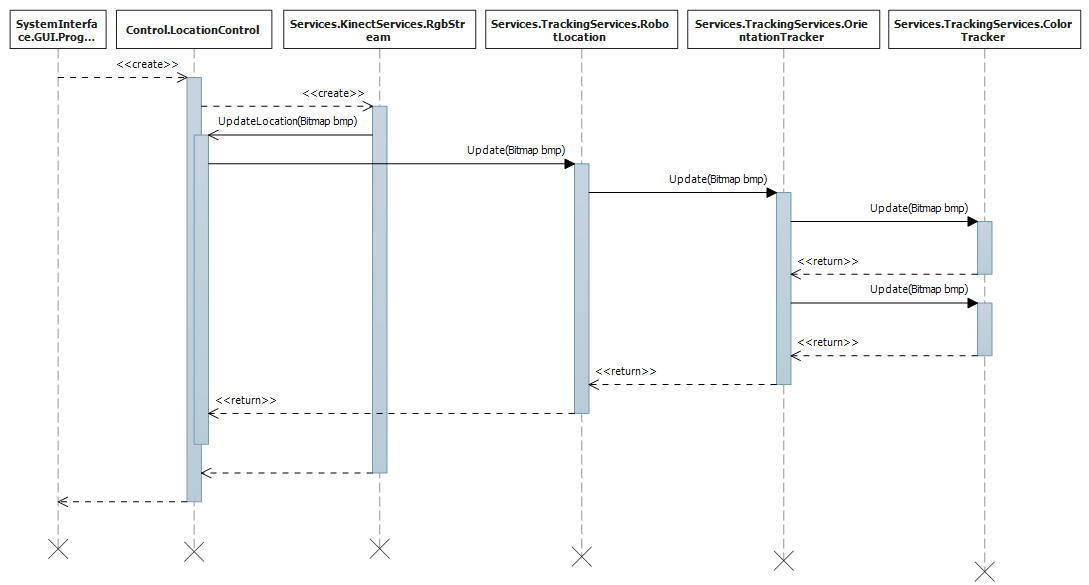
\includegraphics[scale=.7]{sdLocationUpdate}
	\caption{Diagrammet viser opdatering af robottens lokation.}
	\label{img:locUpdate}
	\end{figure} 
	
	\begin{figure}[H]
	\centering 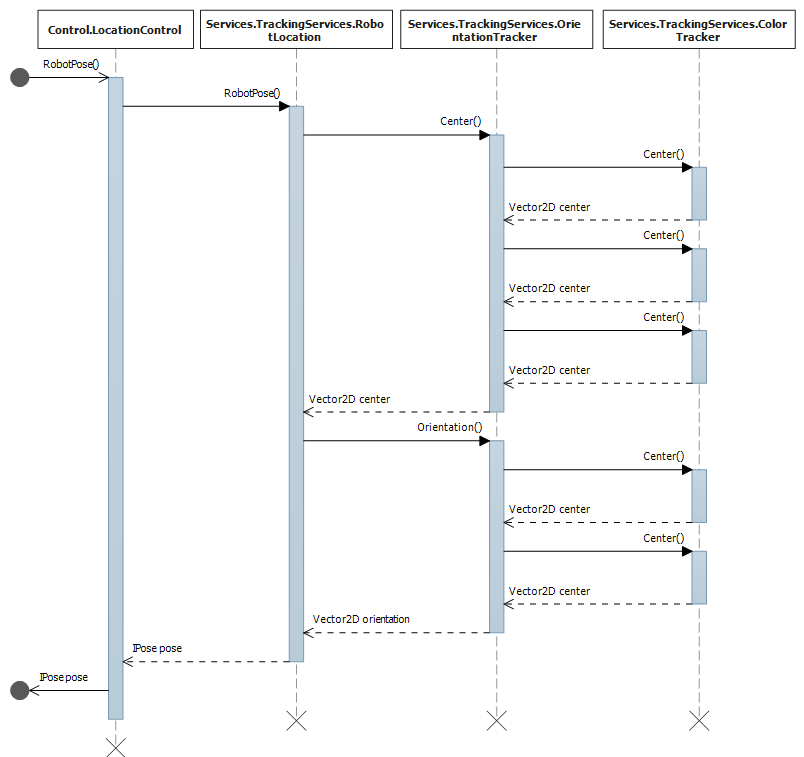
\includegraphics[scale=.65]{sdCalculateLocation}
	\caption{Diagrammet viser udregningen af robottens lokation.}
	\label{img:calcLoc}
	\end{figure}
	
\end{landscape}
\chapter{Kildekode}
Herunder er der en liste over hvad kildekoden indeholder
Kildekoden kan findes her: \url{https://github.com/deaddog/sw505-code/tree/v1.0}.
\begin{itemize}
\item Software der bliver kørt på PC'en ligger under mappen \lstinline[style=c]!.\root! undtagen mappen \lstinline[style=c]!.\root\NXT!.
For at starte programmet gør følgende:
Åben \lstinline[style=c]!Master.sln! og kør \lstinline[style=c]!GUI!.
\item Software der ligger på NXT'en er i mappen \lstinline[style=c]!.\root\NXT!
\item Mindsqualls bilioteket ligger i mappen \lstinline[style=c]!.\Mindsqualls!
\item Vi har en \lstinline[style=c]!GridViewer! til at genskabe grids fra loggen denne kan ses i mappen \lstinline[style=c]!.\GridViewer!.
\item I mappen \lstinline[style=c]!Entropy! er der testprojekter til de forskellige sensorer.
\end{itemize}

\bibliography{bibliography}
\bibliographystyle{plain}
\end{document}
